\documentclass[a4paper,12pt]{article}

\usepackage{jheppub}
\usepackage{taro}
\newcommand\matthree[9]{%
	\begin{pmatrix}
		#1 & #2 & #3 \\ #4 & #5 & #6 \\ #7 & #8 & #9
	\end{pmatrix}%
}

\title{Mathematical Methods in Physics}

\author[a]{Taro V. Brown}

\affiliation[a]{Department of Physics, UC Davis, One Shields Avenue, Davis, CA 95616, USA }


% e-mail addresses: one for each author, in the same order as the authors
\emailAdd{taro.brown@nbi.ku.dk}
\abstract{}
\begin{document} 
\maketitle
\flushbottom
\tableofcontents
\newpage
\section{Residue Calculus}
If $f(z)$ has a pole of order $m$ at $z=a$, thrn
\begin{equation}
\Res[f(z=a)]=\frac{1}{(m-1)!}\lim_{z\to a}\dv[m-1]{}{z}[(z-a)^mf(z)]
\end{equation}
Residue theorem:
If you have some domain with poles in them, you can pinch the conbtour of integration (since it doesn't affect the end results) around these poles. $f$ is analytic in the domain and on the boundary then
\begin{equation}
\oint _C \dd z  f(z)=2\pi i \sum_{a_i\in D}\Res[f(a_i)]\end{equation}
\subsection{Jordan's Lemma} Integrals along the real line, so the contour is just the real axis, so it is open:
\begin{equation}
	\sum_{-\infty}^{\infty}f(x)\dd x= \lim_{R\to \infty }\int_{-R}^{R}f(x)\dd x
\end{equation}
to convert this to a contour integral we have to close the open segment. This can be done by making a semi circle in either the upper or the lower half-plane.
\\
Jordan's Lemma says:
Let $C_R$ be a semicircle of radius R in e.g. upper half plane (UHP) and f is analytic in UHP and decays faster than $|z|^{-1}$ for $\arg(z)\in [0,\pi]$\footnote{This argument just specifies the UHP}, then
\begin{equation}
	\int_{C_R} \dd z e^{i\alpha z}\to 0 \text{ as } R\to \infty, \text{ for } \alpha > 0
\end{equation}
This gets an exponential damping through $i\alpha z=i\alpha \Re (z)-\alpha \Im(z)$, so the integral is bounded by $1/R$ which goes to zero when we take $R\to \infty$\\
\subsubsection{Example I}
Rational functions
\begin{equation}
\int_{-\infty}^{\infty}\frac{p(x)}{q(x)}
\end{equation}
with $p$ and $q$ begin polynomials with $q$ being one degree higher than $p$, also assume $q$ doesn't have a zero along the real line. We can the write using J's Lemma
\begin{equation}
	\int_{-\infty}^{\infty}\frac{p(x)}{q(x)}=\lim_{R\to \infty}\int_{-R}^{R}\frac{p(x)}{q(x)}\to \oint_\gamma \dd z\frac{p(z)}{q(z)}=2\pi i \sum_{a_i\in\text{UHP}}\Res[\frac{p(a_i)}{q(a_i)}]
\end{equation}
where $\gamma$ is closed contour in either UHP or LHP with LHP giving a negative sign.\\
\subsubsection{Example II}
\begin{equation}
\begin{aligned}
\int_{0}^{\infty}\frac{x^2}{(x^2+1)(x^2+9)}&=\frac{1}{2}\int_{-\infty}^{\infty}\frac{x^2}{(x^2+1)(x^2+9)}\\
&\to \frac{1}{2}\oint_\gamma \dd z \frac{z^2}{(z^2+1)(z^2+9)}
\end{aligned}
\end{equation}
This has zeros at $z^2=1$ and $z^2=9$ so 4 simple poles at $z=\{-3i,-i,i,3i\}$. We then include the residues at these poles, so
\begin{equation}
\begin{aligned}
	&\int_{0}^{\infty}\frac{x^2}{(x^2+1)(x^2+9)}\\
	&=\frac{1}{2}2\pi i \left\{
	\Res[\frac{z^2}{(z-i)(z+i)(z+3i)(z-3i)}]_{z=i}+	\Res[\frac{z^2}{(z-i)(z+i)(z+3i)(z-3i)}]_{z=3i}
	\right\}\\
	&=\frac{1}{2}2\pi i \left\{[\frac{z^2}{(z+i)(z+3i)(z-3i)}]_{z=i}+	[\frac{z^2}{(z-i)(z+i)(z+3i)}]_{z=3i}
	\right\}\\
	&=\frac{1}{2}2\pi i \left\{\frac{i^2}{(2i)(4i)(2i)}+\frac{(3i)^2}{(3i-i)(3i+i)(3i+3i)}]
	\right\}
\end{aligned}
\end{equation}
For simple pole one can just drop the pole part and evaluate the remainder at the pole to get the residue.\\
\subsubsection{Example III}
Sin for imaginary values is just Sinh, so $\sin(a z)\to 0$ as $Im(z)\to \pm\infty$ depending on sign of $a:\pm$. Using $\sin(az)=\Im(e^{iz})$
\begin{equation}
	\begin{aligned}
		\int_{0}^{\infty}\frac{x \sin(a x)}{(x^4+4)}&=\Im \oint_\gamma \frac{z e^{iaz}}{(x^4+4)}
	\end{aligned}
\end{equation}
This has poles at $z=\pm 1 \pm i$ so
\begin{equation}
	\begin{aligned}
		\int_{0}^{\infty}\frac{x \sin(a x)}{(x^4+4)}&=\Im \oint_\gamma \frac{z e^{iaz}}{(x^4+4)}
	\end{aligned}
\end{equation}
...\\
...\\
\underline{Example III}
Functions of trig functions
\begin{equation}
	\begin{aligned}
		\int_{0}^{2\pi} \dd \theta F(\sin \theta, \cos \theta )
	\end{aligned}
\end{equation}
with $\sin\theta = \frac{z-\frac{1}{z}}{2}$ $\cos\theta = \frac{z+\frac{1}{z}}{2}$ and $\dd \theta=\frac{\dd z}{iz}$, so
\begin{equation}
	\begin{aligned}
		I=\oint_{|z|=1} \frac{\dd z}{iz} F(\frac{z-\frac{1}{z}}{2}, \frac{z+\frac{1}{z}}{2} )
	\end{aligned}
\end{equation}
E.g.
\begin{equation}
	\begin{aligned}
		\int_{0}^{2\pi} \dd \theta \frac{1}{1+a\cos \theta}\\
		&=\frac{2}{i}\oint_{|z|=1} \frac{\dd z}{iz\left[1+a\frac{z^2+1}{2z}\right]}\\
		&=\oint_{|z|=1} \frac{\dd z}{az^2+2z+a}\\
		&=\frac{2\pi}{\sqrt{1-a^2}}
	\end{aligned}
\end{equation}
the poles are at $z=-\frac{-1\pm\sqrt{1-a^2}}{a}$
\subsection{Principal Value Prescription (Feynman $i\epsilon$ prescription)}
If one tries to integrate a function that blows up on the real line, e.g.
\begin{equation}
\int_{-\infty}^{\infty}\frac{f(x)}{x-a}, ~~~ a\in \mathds{R}
\end{equation}
The way to integrate this is by jumping the pole on axis either below or above, so the integral is slit into
\begin{equation}
	\int_{-\infty}^{a-\epsilon}\frac{f(x)}{x-a}+\int_{a+\epsilon}^{\infty}\frac{f(x)}{x-a}+\int_\Gamma\frac{f(x)}{x-a}
\end{equation}
with $\Gamma$ the contour around the pole on the axis. Then when closing the contour using Jordan's lemma, we have to close it in the plane opposite of the the one we jumped the pole in.
The integral then gives
\begin{equation}
I = P\mp i \pi f(a)
\end{equation}
where P is the principal part (the part of the integral that ignores the divergent pole at $a$). In Feynmans language:
\begin{equation}
\frac{1}{x-a\pm i\epsilon}=P(\frac{1}{x-a})\mp i \pi\delta(x-a)
\end{equation}
\subsubsection{Example I}
Using the Feynman Prescription
\begin{equation}
\begin{aligned}
 \int_{0}^{\infty} \dd x\frac{\sin x}{x} &=\frac{1}{2}\Im\left[ \int_{-\infty}^{\infty} \dd x\frac{e^{ix}}{x}\right]\\
 &=\frac{1}{2}\Im\left[ \int_{-\infty}^{\infty} \dd x\frac{e^{ix}}{x-i\epsilon}\right]\\
  &=\frac{1}{2}\Im\left[P \int_{-\infty}^{\infty} \dd x\frac{e^{ix}}{x-i\epsilon}+i\pi \int_{-\infty}^{\infty} \dd x e^{ix}\delta(x)\right]\\
  &=\pi/2
\end{aligned}
\end{equation}
\subsubsection{Example II}
\begin{equation}
	\begin{aligned}
		\int_{0}^{\infty} \dd k\frac{e^{ikx}}{k^2-m^2} &=\frac{1}{2}\Im\left[ \int_{-\infty}^{\infty} \dd x\frac{e^{ix}}{x}\right]
		&=-\frac{\pi}{x}\sin(m|x|)
	\end{aligned}
\end{equation}
Often the principal is real and since we take the imaginary part, the only contribution comes from the pole 
\section{Conformal Mapping}
Very useful tool in fluid dynamics, since it is very closely tied to solving the Laplace equation in two dimensions.\\
We have seen that if $f$ is analytic then $\Re(f)$ and $\Im (f)$ are harmonic, i.e. they satisfy Laplace's equations in $d=2$ automatically from Causchy-Riemann.
\\\\
\begin{equation}
z\to f(z)
\end{equation}
we can think of this map from some domain in z-plane to $w=f(z)$. It maps points to points. So if $f$ is analytic in the first region\footnote{We only consider simply connected domains, i.e. no holes in the domains.} then it is analytic after the map.
\\\\
\subsection{Riemann Mapping Theorem}
The interior of any domain $\Omega$ (with more than 1 point on $\partial\Omega$), can be conformally mapped to the unit disc $D$ with the boundary being mapped to the unit circle. The map can be made unique by choosing to map a particular point $w_0\in \Omega$ to the origin of $D$ and by orienting a particular directions from $w_0$ to the real axis in $D$.
% TODO: \usepackage{graphicx} required
\begin{figure}[H]
	\centering
	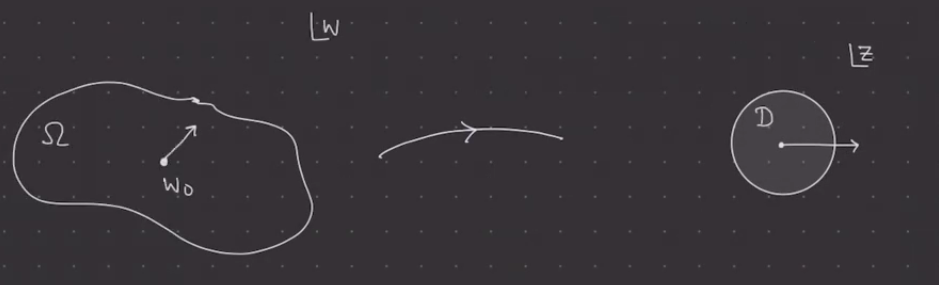
\includegraphics[width=0.7\linewidth]{3}
	\caption{}
	\label{fig:3}
\end{figure}
Let us imagine we are solving the following electrostatics problem:
\begin{equation}
\nabla^2\phi =-\delta(x)\delta(y)
\end{equation}
the potential in two dimensions behaves as
\begin{equation}
\phi\sim -\frac{1}{2\pi}\log r,~~~~~~r=\sqrt{x^2+y^2}
\end{equation}
We can map this to
\begin{equation}
	\Phi= -\frac{1}{2\pi}\log z
\end{equation}
The electrostatic potential with unit charge at $w_0$ and vanishing potential the boundary. From  $\phi$ in this domain we can construct $\Phi(w)$. Physically the situation is like punching a hole in a 2d conductor and placing a charge.
\begin{equation}
\Phi(w)=-\frac{1}{2\pi}\log (ze^{i\alpha})
\end{equation} 
is a conformal map from $w\to z$ plane which preserves the physical solution of the problem. Fixing $\alpha$, fixes a direction.\\\\
\begin{equation}
w=f(z)
\end{equation}
mapos the domain $\Omega$ to $D$. To get the inverse map $z=f^{-1}(w)$ we demand $f'(z)\neq 0$. IF
\begin{equation}
f=u+iv
\end{equation}
Then $\nabla^2u=\nabla^2 v=0$ and $u$ can be viewed as a solution to 3 dimensional Laplace equations if we have cylindrical symmetry. Let us use this to understand some problems we have already seen before.\\\\
Take $\phi=u= \Re f$ as the electrostatic potential, lines of constant $u$ gives equipotential. $v$ is field lines.\\\\
\underline{Example}
Uniform charge density wire along $z=x_3$. The equipotentials are circles and field lines go straight out.
\begin{figure}[H]
	\centering
	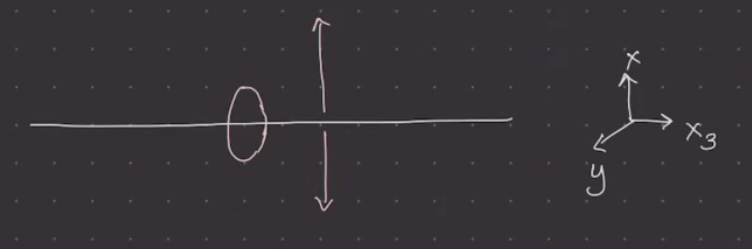
\includegraphics[width=0.7\linewidth]{4}
	\caption{}
	\label{fig:4}
\end{figure}
We have
\begin{equation}
\begin{aligned}
\Phi&=2\lambda \log z\\
\phi&=2\lambda \log r
\end{aligned}
\end{equation}
The equipotentials are $\Re[\Phi]=constant$ give circles in $x,y$ plane. Field lines come from $\Im(\phi)=2\lambda \Theta$.
\\\\
\underline{Example II}
\\\\
Two semi-infinite capacitor places at $y={\pi,-\pi}$ and hold them at constant potential $V(y=\pm \pi)=\pm \pi$. Sketching this, we now the equipotentials just go along the direction of the plates. We can use the exponential map to open it up to (almost) the whole complex plane, so taking $z\to1+z+e^z$. This maps a strip and maps it to the complex plane with two cuts. We can then solve the Laplace equation in the complex plane, i.e. we just get a linear function and the B.C.'s force the solutions to be non-zero.\\\\
The exponential map takes the complex plane and wraps it into a cylinder.
\begin{figure}[H]
	\centering
	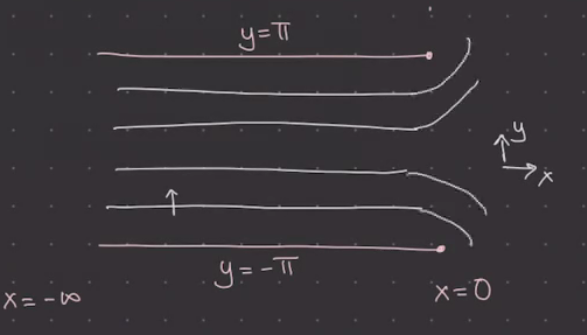
\includegraphics[width=0.7\linewidth]{5}
	\caption{}
	\label{fig:4}
\end{figure}
\begin{itemize}
\item Conformal maps are angle preserving (generally true in arbitrary dimensions)
\item In higher dimensions the full set of conformal maps is the group $SO(d,2)$ which is an extension of the Lorentz group (rotations and boost) SO($d-1,1$).
\item In 2 dimensions the conformal group is much richer: space of analytic maps. So any function $f(z)$ is a conformal transformation. This will be used later to construct interesting domain maps.
\item Subset of conformal maps: fractional linear transformations:
\begin{itemize}
	\item \begin{equation}
		w=\frac{az+b}{cz+d},~~~~~~ad-bc\neq0
	\end{equation}
	\item Translations $w=z+b$ (i.e. $c=0,d=1$)
	\item Scalings $w=\lambda z$ with $\lambda\in \mathds{R}_+$
	\item Rotations $w=e^{i\phi}z$
	\item Inversions $w=\frac{1}{z}$, analytic on $\mathds{C}/\{0\}$ maps interior of punctured disc to its exterior
 \end{itemize}
\end{itemize}
Think of $a,b,c,d$ parameterizing invertable $2\times 2$ matrices living in $GL(2,\mathds{C})$
\begin{equation}
A\begin{pmatrix}
a & b \\c& d
\end{pmatrix}
\end{equation}
If $\det A=ad-bc=1$ them we restrict to $SL(2,\mathds{C})$. \\\\
\underline{Riemann sphere}
The tranformations with $\det A=1$ transform the unit sphere onto it self. $\mathds{P}^1=\mathds{C}\cup \infty$. $S^2\subset R^3$, $\{x_1,x_2,x_3\}$. The sphere can be seen as a sterographic projection from the complex plane onto $S^2$
\begin{equation}
x_1=\frac{z+\bar z}{|z|^2+1},~~~~x_2=\frac{1}{i}\frac{z-\bar z}{|z|^2+1},~~~~x_3=\frac{|z|^2-1}{|z|^2+1}
\end{equation}
\begin{equation}
z=\frac{x_1+ix_2}{1-x_3}
\end{equation}\\\\
\subsection{How to find conformal maps}
First let us take some examples of maps:
\underline{Example I}\\\\
\begin{equation}
w=\frac{z-1}{z+1},~~~~z=\frac{w+1}{1-w}
\end{equation}
This map takes the right half of the $z$-plane to the unit disc in $w$\\\\
\underline{Example II}\\\\
\begin{equation}
\zeta= e^{i\phi}\frac{w-a}{\bar a w-1},~~~~~~|a|<1,~~~\phi\in (-\pi,\pi]
\end{equation}
This leaves the unit disc invariant.\\\\
The general way to find a conformal map is
\begin{itemize}
\item $w=f(z)$ are $\zeta=g(w)$ analytic then $\zeta= g\circ f(z)$ is a conformal map from $z\to \zeta$ planes
\end{itemize}
\underline{Example}\\\\
We want to map a strip in the z-plane to the unit disc. We know that the exponential function maps it to the right half plane
\begin{figure}[H]
	\centering
	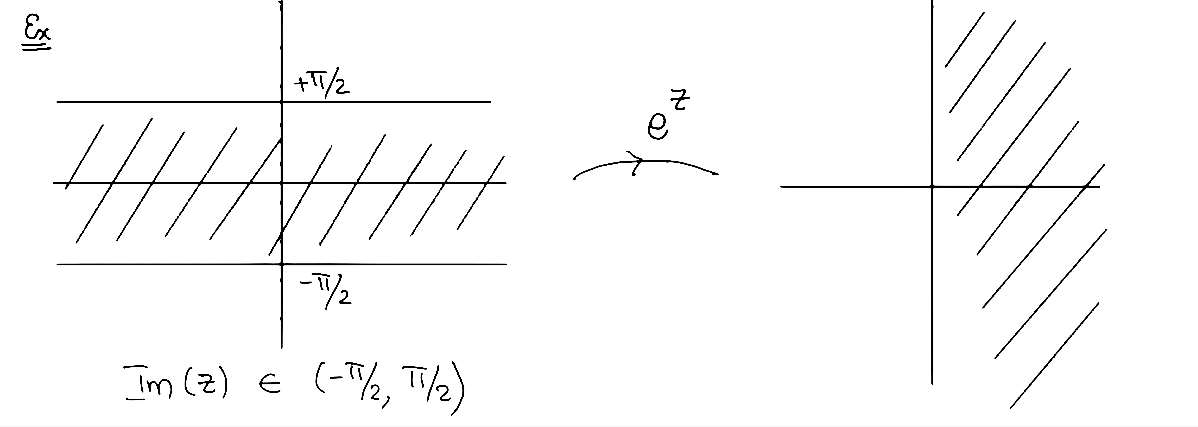
\includegraphics[width=0.7\linewidth]{7}
	\caption{}
	\label{fig:4}
\end{figure}
Now we can use the map from the half-plane to the unit sphere that we just saw and combine the two maps to get
\begin{equation}
\zeta = \frac{e^z-1}{e^z+1}
\end{equation}
\underline{Example}\\\\
To get the map from the UHP to the disc is just a combination of the right half plane map to unit disc, with a rotations:
\begin{equation}
\zeta=\frac{iz-1}{iz+1}
\end{equation}
\subsection{Applications in fluid dynamics}
We will focus on inviscid incompressible fluid and irrotational flows
\begin{equation}
\nabla\cdot \bm u=0,~~~~~~~~\nabla\times \bm u =0
\end{equation}
For 2d flow
\begin{equation}
\bm u=u_x(x,y)\hat e_x+u_y(x,y)\hat e_y
\end{equation}
The conditions on $\bm u$ imply that $u_x,u_y$ satisfy the CR relations. We can write the 2-dimensional vector field $u$ as a complex scalar $U$ as 
\begin{equation}
U(z)=u_x-iu_y
\end{equation}
Further we can write $\bm u=\nabla \phi$ and $\bm u=\nabla \times \begin{pmatrix}
1\\
1
\end{pmatrix}\chi$, with $\phi$ and $\chi$ being complex compliments and we can write
\begin{equation}
\Phi(z)=\phi(x,y)+i\chi(x,y)
\end{equation}
With
\begin{equation}
U(z)=\partial_z\Phi
\end{equation}
\underline{Example}\\\
\begin{figure}[H]
	\centering
	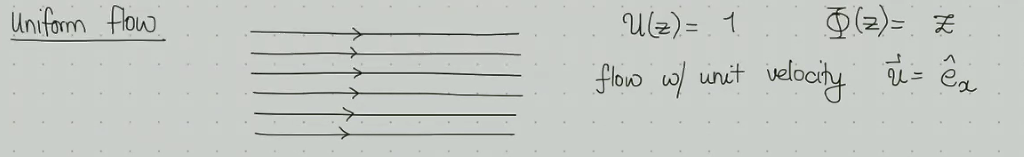
\includegraphics[width=0.8\linewidth]{8}
	\caption{}
	\label{fig:4}
\end{figure}
The streamlines are $y=c$ (constant lines) and the equipotentials are $x=c$. Now recall, analyticity of $\Phi(z)$ leads to $\grad \phi\cdot\grad \chi=0 $ since the velocity is the gradient of $\phi$ and it is tangent to $\chi=c$ then these are the level sets. If we were to add obstacles to the flow, these would be characterized by an absence of fluid flux into/out of the obstacle domain. 
\\\\
\underline{No flux condition}\\\\
$U$ is tangent to the boundary of the obstacle. $\phi$ should satisfy neumann bc at obstacle boundary
\begin{equation}
\pdv{\phi}{\bm n}
\end{equation} 
where $\bm n$ is the normal vector at the boundary.
\begin{figure}[H]
	\centering
	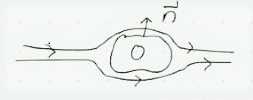
\includegraphics[width=0.6\linewidth]{9}
	\caption{}
	\label{fig:4}
\end{figure}
We will focus on flows which are asymptotically uniform, i.e. $\bm\to\hat e_x$ for $r\to \infty$ with some obstacle intermediate. Here are a few examples:
\begin{figure}[H]
	\centering
	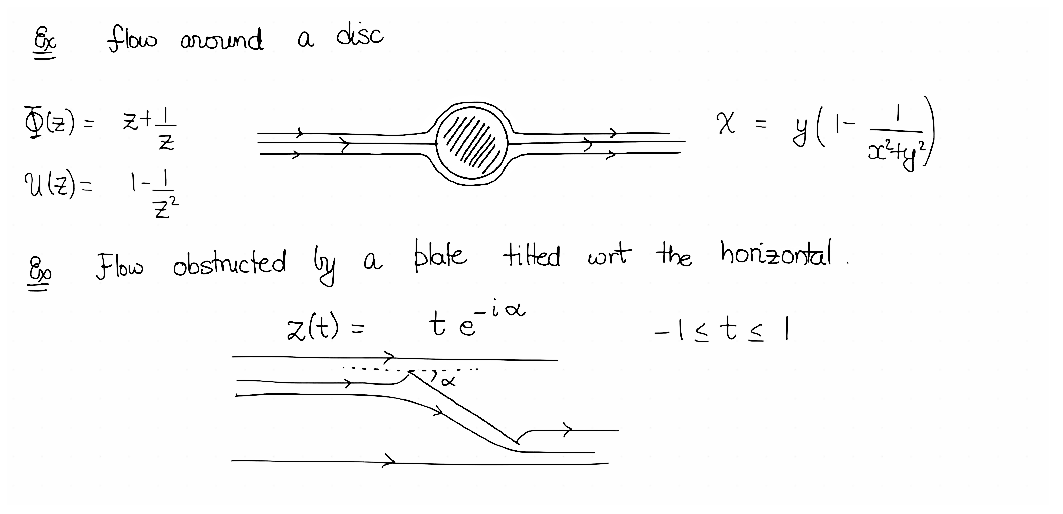
\includegraphics[width=0.9\linewidth]{10}
	\caption{}
	\label{fig:4}
\end{figure}
where $z(t)$ describes the locus of the plate
To solve the last example, we start by solving it for $\alpha=0$, so
\begin{equation}
z(t)=t,~~~~~~-1\leq t \leq 1
\end{equation}
here the solutions is clear since,
$\Phi(z)=z$. If $\alpha\neq 0$ we can solve it by rotating the plate using a conformal map. In aeronautics $\alpha$ is known as the attack angle. We will in this use the fact that rotations do not modify circular domains, which leads to the following trick:\\\\
The  Jakouwski map, mapped the unit disc to the real interval $[-1,1]$. Using this map we can go from the flow we know (at $\alpha=0$) to the unit disc, then rotate this using a rotational map, and finally map back to the $\alpha\neq 0$ solution.\\\\
The flow past a disc has then
\begin{equation}
\Phi(z)=\frac{1}{2}\left(z+z^{-1}\right)
\end{equation}
 We then rotate the disc by $\alpha$ using e.g. the map $w=e^{i\alpha}z$
 and so the jarkowski map goes to
 \begin{equation}
J(z)\to J(e^{-i\alpha})=\frac{1}{2}\left(e^{-i\alpha}w+\frac{e^{i\alpha}}{w}\right)
 \end{equation}
We then recollapse the disc by the inverse Joukoski map ($z(w)=w\pm\sqrt{w^2-1}$) and then finally rotate the solution back so that the streamlines are asymptotically horizontal, we lastly get:
\begin{equation}
\Phi(z)=e^{i\alpha}\left(z\cos \alpha -i\sin \alpha \sqrt{z^2-e^{-2i\alpha}}\right)
\end{equation}
As a pictorial example see below
\begin{figure}[H]
	\centering
	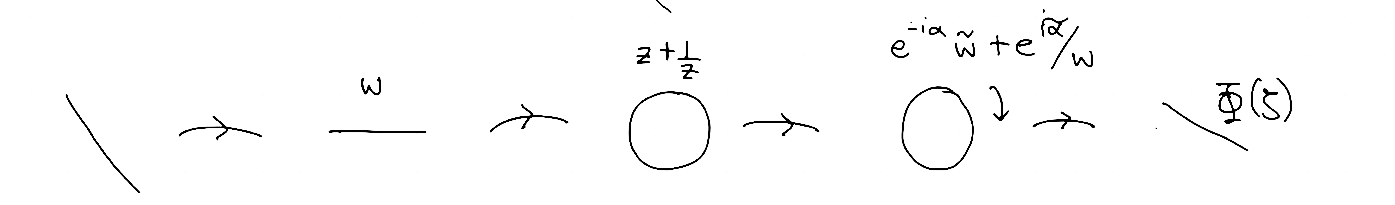
\includegraphics[width=0.9\linewidth]{11}
	\caption{}
	\label{fig:4}
\end{figure}
\section{Branch structure \& multivalued functions}
Some functions are analytic in some domain but do not have poles or essential singularities but rather something known as branchcuts. The canonical example is the function
\begin{equation}
f(z)=\log z
\end{equation}
If one writes $z=|z|e^{i\arg z}$, with $\arg z=\theta +2\pi n$,  $n\in \mathds Z$ and $\theta \in [-\pi,\pi]$. Hence we get
\begin{equation}
	f(z)=\log |z|+i\arg(z)
\end{equation}
Because $z$ and $z^{2\pi i n}$ have the same $\theta$ there is an ambiguity and hence $i\arg(z)$ is multivalued.
\begin{figure}[H]
	\centering
	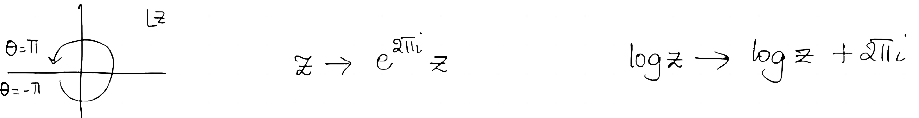
\includegraphics[width=0.9\linewidth]{12}
	\caption{}
	\label{fig:4}
\end{figure}
The origin is a branch point of $\log z$ as going around gives a discontinuous jump. Now note that
\begin{equation}
\log \frac{1}{z}=-\log z
\end{equation}
and hence there is a similar problem at $z=\infty$. This means that we can think of $\log z$ as a function in the complex plane with a line cut out of it. This line is the branchcut between the two branch points. This cut "prevents" us from going all the way around the circle, and so we never experience the discontinuity. If we instead restrict $-\pi <\theta<\pi $ on could draw this as
\begin{figure}[H]
	\centering
	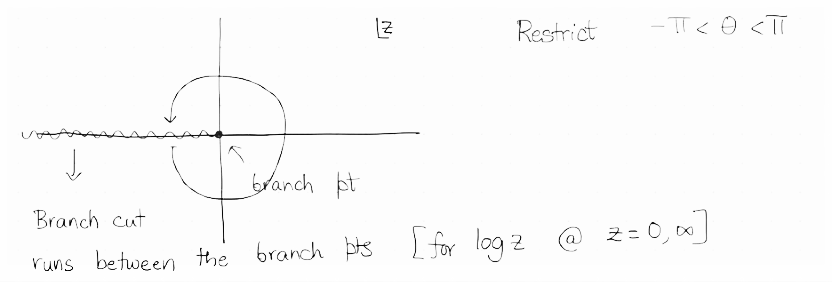
\includegraphics[width=0.9\linewidth]{13}
	\caption{}
	\label{fig:4}
\end{figure}
One can also think of this using Riemann sheets. We look at an infinite copy of complex planes and on each sheet we cut out the negative part of the real line.
\begin{figure}[H]
	\centering
	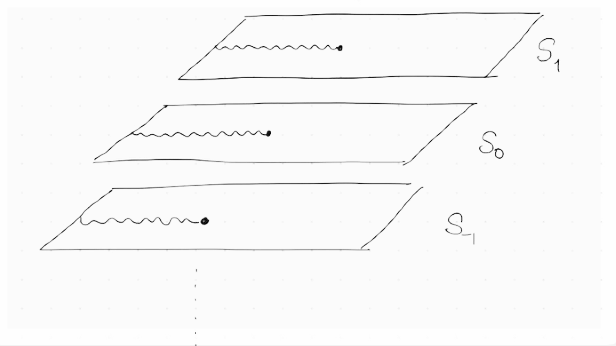
\includegraphics[width=0.9\linewidth]{14}
	\caption{}
	\label{fig:4}
\end{figure}
We then define
\begin{equation}
f_n(z)=\log |z|+i(\theta +2\pi n),~~~~\theta\in (-\pi,\pi)
\end{equation}
Slightly above and below the cut we have
\begin{equation}
\begin{aligned}
	f_n(|z|,\pi-\epsilon)&=\log |z|+i(\pi-\epsilon +2\pi n),~~~~\theta\in (-\pi,\pi)\\
		f_n(|z|,-\pi+\epsilon)&=\log |z|+i(-\pi+\epsilon +2\pi n),~~~~\theta\in (-\pi,\pi)\\
\end{aligned}
\end{equation}
across the cur we then have a discontinuiy
\begin{equation}
	\begin{aligned}
		\text{disc} f_n= \lim_{\epsilon\to 0}f_n(|z|,\pi-\epsilon)-f_n(|z|,-\pi+\epsilon)
		\end{aligned}
\end{equation}
We will then identify the "positive" side of the plane $f_{n}^+$ with $f_{n+1}^-$, so that we get the follow stairwell structure:
\begin{figure}[H]
	\centering
	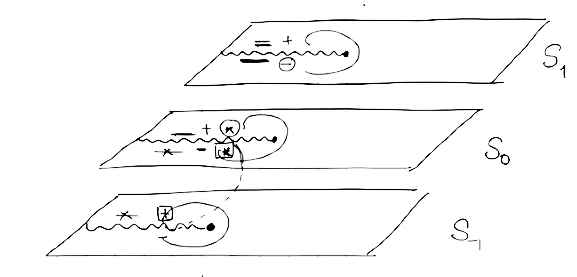
\includegraphics[width=0.9\linewidth]{15}
	\caption{}
	\label{fig:4}
\end{figure}
I.e. the $f_n$ value on the n'th sheet above the cut is equal to the $f_n$ value on (n+1)'st sheet below cut.\\\\
Since the logarithm has the property, exponentials also do. Consider for instance monomials
\begin{equation}
z^{\alpha}=e^{\alpha\log z}
\end{equation}
We then have the following cases
\begin{itemize}
\item $\alpha\in \mathds R / \mathds Q$   irrational: we have the same logarithmic cut
\item  $\alpha\in \mathds Q$ we have a finite number of sheets
\begin{itemize}
\item Example $\sqrt{z}:~~|z|^{1/2}e^{i\arg z/2}$. We can define the two phases
\begin{equation}
\sqrt{z}=\begin{cases}
&|z|^{1/2}e^{i\theta /2}\\
&|z|^{1/2}e^{i\theta z/2+i\pi}
\end{cases}
\end{equation}
The cut can be placed anywhere in the complex plane, one just has to be consistent in the convention used. 
\item Cuts can also be finite. The function $(z^2-1)^{1/2}$ e.g. has branchpoints at $z\pm 1$
\end{itemize}
\end{itemize}
Branch cuts show up a lot in 2d CFT's. Since fermions live on the double cover. Another way to put it is that since fermions behave as $\psi^\mu(x)=\psi^\mu(x+2\pi)=-\psi^\mu(x)$, which means it behaves like the squareroot function.
\subsection{Integrating functions with branch-cuts}
\subsubsection{Example I}
\begin{equation}
\begin{aligned}
I=\int_{0}^{\infty}\dd x \frac{x^\alpha}{1+x^2},~~~~~|\alpha|<1
\end{aligned}
\end{equation}
We convert this to a complex function
\begin{equation}
	\begin{aligned}
		I_c=\oint_{C}\dd z \frac{z^\alpha}{1+z^2},~~~~~|\alpha|<1
	\end{aligned}
\end{equation}
We first have to decide where to put the cut. Ideally we want the contour not to jump the cut. If we put the cut along the positive real axis then place our closed contour around the cut in the following way.
\begin{figure}[H]
	\centering
	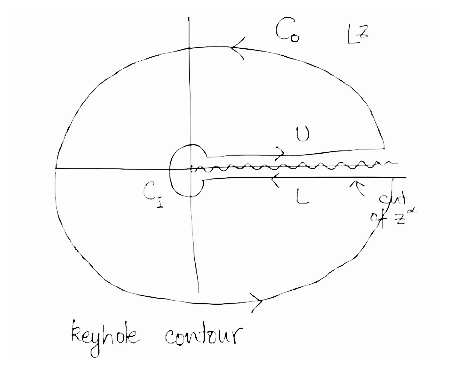
\includegraphics[width=0.7\linewidth]{16}
	\caption{}
	\label{fig:4}
\end{figure}
The contour is then
\begin{equation}
C=C_0\cup C_1\cup L\cup U
\end{equation}
On $C_0$ we have $z=Re^{i\theta}$
\begin{equation}
\begin{aligned}
	I_{C_0}=\int_{C}\dd z \frac{z^\alpha}{1+z^2}=\int_{0}^{2\pi}\dd \theta \frac{R^{1+\alpha}}{1+R^2e^{2i\theta}}e^{i(\alpha+1)\theta }
\end{aligned}
\end{equation}
This big circle doesn't contribute since
\begin{equation}
\frac{R^{\alpha+1}}{R^2}\sim \frac{1}{R^{1-\alpha}}\to 0~~~~\text{as }R\to 0 
\end{equation}
Similarly
\begin{equation}
	\begin{aligned}
		I_{C_0}=\int_{C}\dd z \frac{z^\alpha}{1+z^2}=\int_{0}^{2\pi}\dd \theta \frac{R^{1+\alpha}}{1+R^2e^{2i\theta}}e^{i(\alpha+1)\theta }
	\end{aligned}
\end{equation}
\section{Analytic continuation}
\subsection{Introduction}
Often times one encounters a computation where there are certain limitations using real analysis, e.g. the integral has a part that is diverging. The basic idea of analytic continuation relies on the fact that complex analytic functions are very constrained, i.e. it suffices to them in a small neighborhood. This allow one to extend the definition to a larger domain while maintaining analyticity.
\\\\
As an example, let us imagine the following three domains, where we know that $f_1$ is analytic in $D_1$ and that $f_2$ is analytic in $D_2$. Further we know that $f_1=f_2$ in some common domain $D\subset D_1,D_2$. Then we conclude there must be a function which is analytic in the domain $D_1\cup D_2$.
\begin{figure}[H]
	\centering
	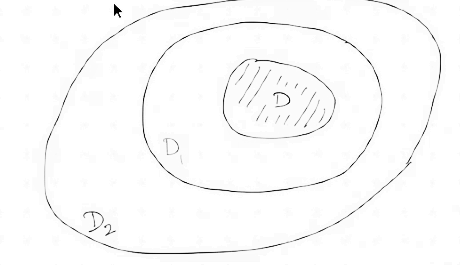
\includegraphics[width=0.5\linewidth]{17}
	\caption{}
	\label{fig:4}
\end{figure}
\subsubsection{Example I}
Take the functions
\begin{equation}
\begin{aligned}
f_2&=\sum_0^{\infty}z^n=\frac{1}{1-z}~~~~|z|<1\\
f_2&=\sum_0^{\infty}\left(\frac{3}{5}\right)^{n+1}\left(z+\frac{2}{3}\right)^n=\frac{1}{1-z}~~~~|z+2/3|<5/3
\end{aligned}
\end{equation}
These two functions have the same representation but are valid for different domains
\begin{figure}[H]
	\centering
	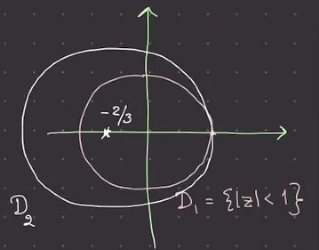
\includegraphics[width=0.5\linewidth]{18}
	\caption{}
	\label{fig:4}
\end{figure}
The function $f_2$ has been analytically continued and is valid for the much larger domain $D_2$
\subsubsection{Example II}
We will often encounter integrals which can be analytically continued.
\begin{figure}[H]
	\centering
	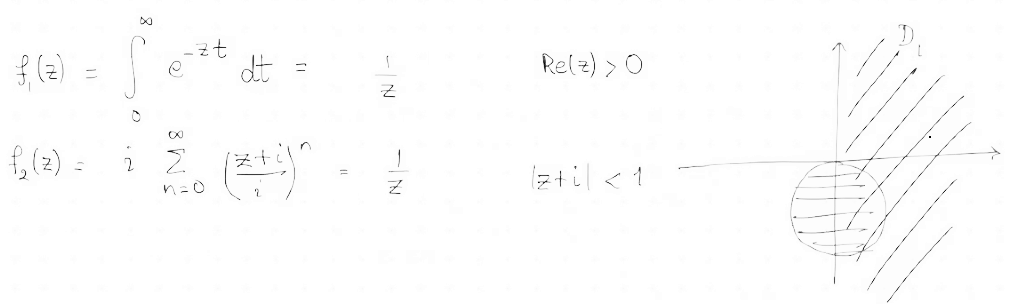
\includegraphics[width=0.8\linewidth]{19}
	\caption{}
	\label{fig:4}
\end{figure}
If you were given the first integral, one would naively think that for certain values of $z$ we would not be able to perform it, however we see that from the infinite sum one can define a version which is valid in part of the domain that was previously excluded.\\\\
\subsubsection{Example III}
Take $\phi(x)$ to be a test function which decays rapidly enough at infinity. We then take the following integral defining an "inner product"
\begin{equation}
(x^{\alpha-1},\phi)=\int_0^\infty x^{\alpha-1}\phi(x)\dd x
\end{equation}
Notice there is an IR divergence if $\Re(\alpha)<0$. We then introduce $\epsilon$ which is known as an IR regulator and take the $\epsilon\to 0$ in the end.
\begin{equation}
\begin{aligned}
I&=\int_\epsilon^\infty x^{\alpha-1}\phi(x)\dd x\\
&=\underbrace{\frac{x^\alpha}{\alpha}\big|^{\infty}_\epsilon}_{0 \text{ for } \alpha > 0}
-\frac{1}{\alpha}\int_\epsilon^\infty x^{\alpha}\partial_x\phi(x)\dd x\\
&=-\frac{1}{\alpha}\int_\epsilon^\infty x^{\alpha}\partial_x\phi(x)\dd x
\end{aligned}
\end{equation}
This is convergent even when $-1<\Re \alpha  <0$, so this extends the definition of the original integral $I$ and together with the previous definition gives an analytic function for $\Re \alpha >-1$. There are a few caveat however, as we must assume that also the derivative of $\phi(x)$ must be sufficiently damped. The new function has pole at the origin $\alpha=0$ with residue
\begin{equation}
-\int_0^\infty \partial_x\phi(x)=\phi(0)
\end{equation}
One could use integration by parts again (and again, and again) to get
\begin{equation}
\begin{aligned}
I(\alpha)&=\frac{1}{\alpha(\alpha+1)}\int_{0}^{\infty}x^{\alpha+1}\phi''(x)\dd x
\\
&\vdots
\end{aligned}
\end{equation}
Each iteration pushed the domain one more integer into the negative $x$ axis and has poles at $\alpha=-n$ with residues \\\\
...\\\\
\subsection{Gamma function}
A famous example is the function
\begin{equation}
\Gamma(z)=\int_0^{\infty}t^{z-1}e^{-t}\dd t~~~~~\Re(z)>0
\end{equation}
Repeating the same steps as before, we can write this as
\begin{equation}
	\Gamma(z)= \frac{1}{z}\int_0^{\infty}t^{z}e^{-t}\dd t=\frac{1}{z}\Gamma(z+1)
\end{equation}
Iterating this recursion one gets.
\begin{equation}
\Gamma(z)=\frac{\Gamma(z+n)}{(z+n-1)!}
\end{equation}
The residues are (at $z=-n$) given by $(-1)^n/n!$ and so we have analytically extended the gamma function to the whole complex plane with simple poles. Another definition of the gammafunction is
\begin{equation}
\frac{1}{\Gamma(z)}=\frac{1}{2\pi i}\int_C \dd \xi\, \frac{e^\xi}{z^\xi}
\end{equation}
This is defined in a very different domain. The contour $C$ is the Hankel (or hairpin) contour, see below
\begin{figure}[H]
	\centering
	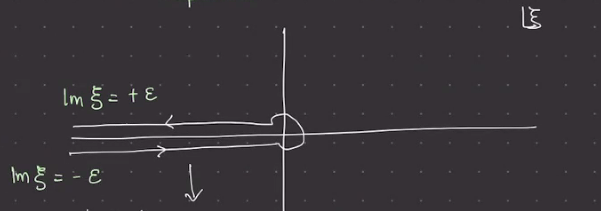
\includegraphics[width=0.7\linewidth]{20}
	\caption{}
	\label{fig:4}
\end{figure}
For positive $n$ where is no cut and the integrand can just be evaluated on the poles. By the residue theorem one finds the same as the previous definition of the gamma function.
\begin{equation}
	\frac{1}{\Gamma(z)}=\frac{1}{(n-1)!}
\end{equation}
 This is not enough to conclude the integrals describe the same function however, so let us integrate by parts
\begin{equation}
\begin{aligned}
	\frac{1}{\Gamma(z)}&=\frac{1}{2\pi i}\frac{e^{\xi}}{(z-1)\xi^{z-1}}\Big|_{-\infty-i\epsilon}^{-\infty+i\epsilon}
+
\frac{1}{z-1}\frac{1}{2\pi i}\int_C \dd \xi\, \frac{e^\xi}{z^{\xi-1}}\\
&=\frac{1}{(z-1)\Gamma(z-1)}
\end{aligned}
\end{equation}
And so we see that the recursion formula from before works for this way of expressing the gamma function as well.
\subsection{Schwarz Reflection Principle}
Suppose we have a function $f_1$ which is analytic in $D_1$ (and along the boundary $B$). If we then reflect this function $e.g.$ on the real axis, and call it $f_2$, then $f_1=f_2$ on $B$. Or $f_1=f_2$ on $D_1\cup D_2$.
\begin{figure}[H]
	\centering
	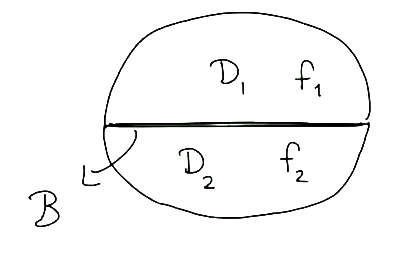
\includegraphics[width=0.3\linewidth]{21}
	\caption{}
	\label{fig:4}
\end{figure}
Say one has $f$ analytic in some domain $D$ which contains a part of the real line $\mathds R_{[a,b]}$. Further let us assume $f(z)$ is real when $z\in \mathds{R}$. Then we can construct a new function, $g(z)$, which extends $f(z)$ below the real axis:
\begin{equation}
g(z)=\begin{cases}
f(z)~~~~z\in D\\
\overline{f(\overline{z})}~~~~z\in D^*
\end{cases}
\end{equation}
This shows up for instance in the context of dispersion relation which we will now go through.
\subsection{Dispersion Relations and Optical Theorems}
If you have light traveling through some non-linear medium, then the wave-profile will get attenuated (loss of flux density through medium) as it propagates
\begin{equation}
e^{i n(\omega)\bm k\cdot \bm x-i\omega t},~~~~~~n(\omega)=n_r+in_I: \text{ Complex refraction coeffecient}
\end{equation}
One can thing of the refraction coeffecient as an analytic function of (complex) $\omega $ and the physical refraction coefficient is the limit as you approach the the real part from above
\begin{equation}
n_{\text{phys}}(\omega )=\lim_{\epsilon\to 0^+}n(\omega +i\epsilon)
\end{equation}
In these cases the behavior of $n$ will usually look something like the following
\begin{figure}[H]
	\centering
	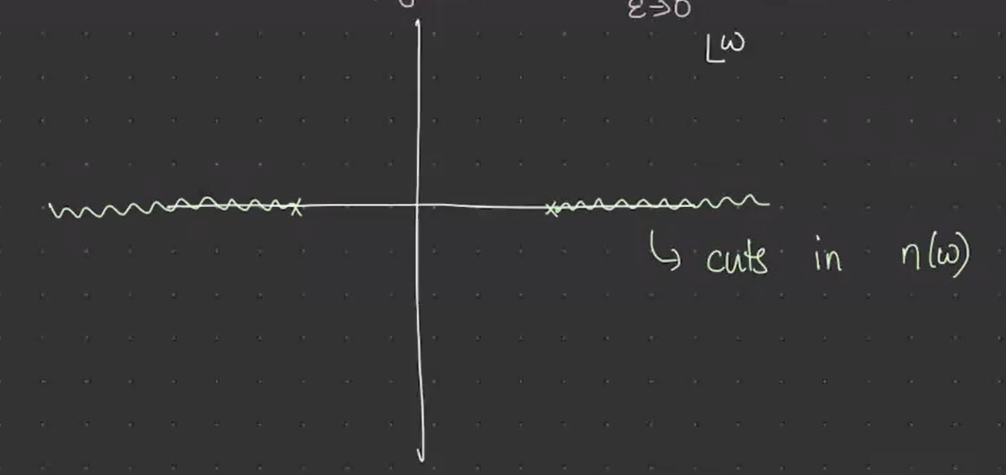
\includegraphics[width=0.5\linewidth]{22}
	\caption{}
	\label{fig:4}
\end{figure}
It has cuts on the real axis, which give non-trivial scattering in the medium in this region.
Another example of analytic continuation one can consider a damped harmonic oscillator with external driving
\begin{equation}
\ddot{x}+\gamma \dot{x}+(\Omega^2+\gamma^2)x=F(t)
\end{equation}
The solutions can be written as
\begin{equation}
x_{\text{sol}}(t)=\int_{-\infty}^{\infty}G(t-t')F(t')F(t')\dd t'
\end{equation}
We implement the boundary condition $G(t)=0$ for $t<0$, essentially turning on the driving force at $t=0$. The fourrier tranformed greensfunction is
\begin{equation}
G(w)=\int_{-\infty}^{\infty}G(t)e^{i\omega t}
\end{equation}
This is analytic in the UHP and can be solved by
\begin{equation}
G(\omega)=-\frac{1}{(\omega+i\gamma)^2-\Omega^2}
\end{equation}
which has poles as indicated on the figure below
\begin{figure}[H]
	\centering
	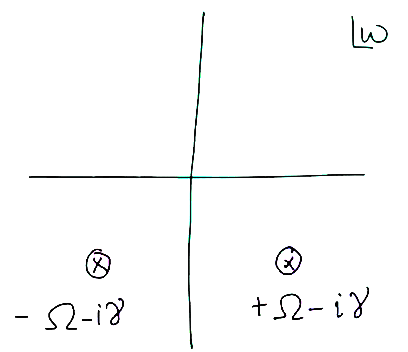
\includegraphics[width=0.3\linewidth]{23}
	\caption{}
	\label{fig:4}
\end{figure}
Suppose we have a function $f(z)$ which has a cut on part of the real axis. We can use the Schwarz reflection principle to tell us something about the function. First we evaluate this using the keyhole contour and can represent the function in the following manor (given it has a residue at $\xi=z$):
\begin{equation}
\begin{aligned}
f(z)=\frac{1}{2\pi i}\int_C \frac{f(\xi)}{\xi-z}\dd \xi
\end{aligned}
\end{equation}
If $f$ was known above the real axis and we get it below by using the reflection principle, we can write
\begin{equation}
	\begin{aligned}
		f(z)=\frac{1}{2\pi i}\left[\int_{x_0}^{\infty}\dd x \frac{f(x+i\epsilon)}{x-z+i\epsilon}-\int_{x_0}^{\infty}\dd x \frac{f(x-i\epsilon)}{x-z-i\epsilon}\right]
	\end{aligned}
\end{equation}
where we assume that $z$ is not on the real axis and that $f(z)$ decays fast enough to use Jordan's Lemma. From combining the two we get
\begin{equation}
	\begin{aligned}
		f(z)=\frac{1}{\pi}\int_{x_0}^{\infty}\dd x \frac{\Im f(x+i\epsilon)}{x-z}
	\end{aligned}
\end{equation}
This is known at the dispersion relation. If $f(z)$ is not damped at infinity for large $\Im(z)$ then we can instead derive the once subtracted dispersion
\begin{equation}
	\begin{aligned}
		f(z)-f(z_0)=\frac{z-z_0}{\pi}\int_{x_0}^{\infty}\dd x \frac{\Im f(x+i\epsilon)}{(x-z)(x-z_0)}
	\end{aligned}
\end{equation}
Now the denominator goes as $x^2$ which helps with convergence at large $x$. These types of equations show up for instance when there is propagation through some medium with attenuation. For light propagation one gets the \textit{Optical Theorem}
\begin{equation}
	\begin{aligned}
		\Im [f(\omega)]=\frac{\omega}{4\pi}\sigma_{\text{abs}}(\omega)
	\end{aligned}
\end{equation}
where $f(w)$ is the forward scattering amplitude and $\sigma(w)$ is the total absorption cross-section. 
%%%%%%%%%%%%%%%%%%%%%%%%%%%%%%%%%%%%%%%%%%%%%%%%%%%%%%%%%%%%%%%%%%%%%%%%%%%%%%%%%%%%%%%%%%%%%%%%%%%%%%%%%%%%%%%%%%%%%%%%%%%%%%
\section{Asymptotic expansions}
Consider the following anharmonic integral which we can take as a toy model for quantum mechanics. 
\begin{equation}
	\begin{aligned}
		f(\lambda)=\int_{-\infty}^{\infty}\dd e^{-x^2-\lambda x^4}
	\end{aligned}
\end{equation}
One can't use Gaussian tricks because of the $x^4$ term. Let us instead then write this part as a Taylor series, assuming $\lambda \ll 1$
\begin{equation}
	\begin{aligned}
		f(\lambda)&=\int_{-\infty}^{\infty}\dd e^{-x^2}\left[\sum_{n=0}^{\infty}\frac{(-1)^n}{n!}\lambda^n x^{4n}\right]\\
		&=\sum_{n=0}^{\infty}\frac{(-1)^n}{n!}\lambda^n\int_{-\infty}^{\infty}\dd e^{-x^2} x^{4n}\\
		&=\sum_{n=0}^{\infty}\frac{(-1)^n}{n!}\lambda^n\,\Gamma(2n+\frac{1}{2})\\
	\end{aligned}
\end{equation}
Where the Gamma-function integral is obtained through a change of variables. Now we have a problem though, since the gamma function is approximately $\Gamma\sim (2n)!$ so the series is non-convergent. This is related to the non-careful swapping of the order of limits. The series representation obtained is asymptotic though since 
\begin{equation}
	\begin{aligned}
		f(\lambda)\sum_{n=0}^{\infty}\sim a_n\lambda^n
	\end{aligned}
\end{equation}
From this $f(\lambda)$ can be aveluated by fixing lambda and then taking a certain number of term in the series.
\begin{equation}
	f(\lambda)\sim \sum_{n=0}^{N} a_n\lambda^n+\mathcal{O} (\lambda^{N+1})
\end{equation}
where the following limit is bounded, but can be large
\begin{equation}
	\begin{aligned}
		\lim_{\lambda\to 0}\frac{|f(\lambda)-\sum_{n=0}^{N} a_n\lambda^n|}{|\lambda^{N+1}|}=K<\infty
	\end{aligned}
\end{equation}
For a fixed number of terms in the series, one decides how small $\lambda$ need to be, to get a good approximation. All perturbation series calculations we will ever do are in this regime. Note that one cannot deduce from the series (naïvely) the fact that there may be non-perturbation effects that scale like $e^{-\verb|#|/\lambda}$.

Another important application is in statistical mechanics. Say you are looking at the canonical partition function
\begin{equation}
	\begin{aligned}
		Z(\beta)=\sum_n \dd n\, e^{-\beta E_n}
	\end{aligned}
\end{equation}
here the $d_n$ denote degeneracies at level $n$. To compute $d_n$ from $Z(\beta)$ we can calculate the spectral density and then read of the number of states with a given energy.
\begin{equation}
	\begin{aligned}
	\rho(E)	\int\dd \beta \,Z(\beta)e^{\beta e}
	\end{aligned}
\end{equation}
At large E this is however not regulated and this is the type of problem that we would like to deal with.
\subsection{Stirlings asymptotic for $\Gamma(x)$}
Let us remind ourselves of the following form og the $\Gamma$ function
\begin{equation}
	\begin{aligned}
		\Gamma(x+1)&=\int_{0}^{\infty}e^{-t} t^x \,\dd t\\
		&=x^{x+1}\int_{0}^{\infty}e^{x\left[\log \zeta-\zeta\right]} \,\dd \zeta
	\end{aligned}
\end{equation}
where we have performed a change of variables in the second line $t=x\zeta$. We would know like to know how this behaves for large $x$. The integrand $e^{xf(\zeta)}$ for large $x$ is exponentially large near local maxima $\Re f(\zeta)$. If we fix $x$ this means that the integrand is sharply peaked around this maximum.  In our case 
\begin{equation}
	\begin{aligned}
		f(\zeta)=\log \zeta -\zeta =-1-\frac{1}{2}(\zeta-1)^2+\mathcal{O}(\zeta^4)
	\end{aligned}
\end{equation}
which has a maximum at $\zeta=1$.
\begin{equation}
	\begin{aligned}
				\frac{\Gamma(x+1)}{x^{x+1}}
		&=x^{x+1}\int_{0}^{\infty}e^{-x}e^{-x\frac{1}{2}(\zeta-1)^2+\cdots} \,\dd \zeta
	\end{aligned}
\end{equation}
There is a local maximum at $\zeta=1$ and we have quadratic corrections which fall off fast away from the maximum. Performing the Gaussian integration and dropping the higher order corrections one obtains
\begin{equation}
	\begin{aligned}
		\Gamma(x+1)
		&=e^{x+\frac{1}{2}}e^{-x}\sqrt{\frac{2\pi}{x}}
	\end{aligned}
\end{equation}
Retaining higher order terms, one could obtain an asymptotic expansion.
\begin{equation}
	\begin{aligned}
		\Gamma(x+1)
		&\sim e^{x+\frac{1}{2}}e^{-x}\sqrt{2\pi}\left[1+\frac{1}{12x}+\frac{1}{288x^2}+\cdots \right]
	\end{aligned}
\end{equation}
\subsection{Saddle point evaluation of integrals by the method of steepest descend}
Think of the integrand of some function, then we go to some local maximum and we then go down from this maximum following the path where the real part decreases the fastest, while the imaginary part doesn't oscillate to quickly. The formal structure is integrals of the following form
\begin{equation}
	\begin{aligned}
		\int_C e^{\alpha f(z)}g(z)\,\dd z,~~~~~~|\alpha|\ll 1
	\end{aligned}
\end{equation}
and we demand that $\Re f(z)$ decreased rapidly enough from the maximum at some $z=z_0$ and that $\Im f(z)$ stays roughly the same.
%%%%%%%%%%%%%%%%%%%%%%%%%%%%%%%%%%%%%%%%%%%%%%%%%%%%%%%%%%%%%%%%%%%%%%%%%%%%%%%%%%%%%%%%%%%%%%%%%%%%%%%%%%%%%%%%%%%%%%%%%%%%%%
%%%%%%%%%%%%%%%%%%%%%%%%%%%%%%%%%%%%%%%%%%%%%%%%%%%%%%%%%%%%%%%%%%%%%%%%%%%%%%%%%%%%%%%%%%%%%%%%%%%%%%%%%%%%%%%%%%%%%%%%%%%%%%
%%%%%%%%%%%%%%%%%%%%%%%%%%%%%%%%%%%%%%%%%%%%%%%%%%%%%%%%%%%%%%%%%%%%%%%%%%%%%%%%%%%%%%%%%%%%%%%%%%%%%%%%%%%%%%%%%%%%%%%%%%%%%%
%%%%%%%%%%%%%%%%%%%%%%%%%%%%%%%%%%%%%%%%%%%%%%%%%%%%%%%%%%%%%%%%%%%%%%%%%%%%%%%%%%%%%%%%%%%%%%%%%%%%%%%%%%%%%%%%%%%%%%%%%%%%%%
\section{Groups, Lie Algebra and Representations}
\subsection{Definition of groups}
A group is defined as follows:\\\\
A set of elements with some operation, referred to as mulitplication that acts in the following manor
\begin{itemize}
\item $x,y\in G~~ \to~~x\cdot y \in G$ 
\item $\exists\, I\in G~~ \to~~x\cdot I=I\cdot x =x~~~~\forall\in G$ 
\item $\forall\, x\in G~~\exists\,x^{-1}\to x^{-1} x=x x^{-1}=I$
\item the multiplication is associative $(x\cdot y)\cdot z=x\cdot (y\cdot z)$
\item Not necessarily commutative $x\cdot y\neq y\cdot x$, if it is, the group is Abelian.
\end{itemize}
\subsection{Subgroups and conjugacy classes:}
A subset  $S\subset G$ is a subgroup if $S$ is closed under multiplication. An example is the group of integers which is a subgroup of the real numbers, with both the group and the subgroup having addition as its multiplication rule.

Two elements $x,y\in G$ are conjugate if $\exists\,g\in G\to x=g\cdot y\cdot g^{-1}$, with $g$ the conjugating element. This can be used to define equivalence classes. As an example think of rotations in 3 dimensions, all rotations that are classified by a specific angle are equivalent to each other, which can be seen by performing a suitable rotation of basis.

\subsection{Permutation group}
Define the group by action on $\{1,2,\dots,n\}$. This action can be represented by $\sigma=(\sigma(1)\,\sigma(2)\,\sigma(3)\,\dots,\sigma(n))$. There are $n!$ elements, which is also known at the order of the group. 
\begin{equation}
\sigma: 
\begin{pmatrix}
1 & 2 & 3 \cdots & n\\
\sigma(1) & \sigma(2) & \sigma(3) \cdots & \sigma(n)
\end{pmatrix}
\end{equation}
The elements of $S_2$ are
\begin{equation}
S_2:~~~~~\begin{pmatrix}
1 & 2\\
1 & 2
\end{pmatrix}
~~~\begin{pmatrix}
	1 & 2\\
	 2& 1
\end{pmatrix}
\end{equation}
Every permutation can be decomposed into 
\begin{itemize}
\item a sequence of cycles
\item into a sequence of transpositions (cycles of length 2)
\end{itemize}
Example\\\\
We take an element of $S_8$ and notice that there for this element a few closed cycles:
\begin{equation}
\begin{pmatrix}
	1 & 2 & 3 & 4 & 5 & 6 & 7 & 8\\
	3 & 5 & 7 & 1 & 2 & 8 & 4 & 6
\end{pmatrix}\in S_8 =(1374)(25)(68)
\end{equation}
Cycles are classified by their lengths:
\begin{itemize}
\item (1) cycle takes elements to it self, so are often omitted.
\item (2) cycles are known as transpositions and every longer cycle can be decomposed in terms of these. 
\end{itemize}
Permutations can be assigned a parity (even/odd) by counting the number of transpositions. Two permutations are conjugate if and only if they have the same cycle structure, meaning that if $\sigma,\pi\in S_n$ are conjugate, i.e $\exists\,\xi \in S_n\to  \sigma \xi \cdot \pi \xi^{-1}$, then cycles$\,\sigma$=cycles$\,\pi$. If we denote the number of $n$-cycles in a permutation by $r_n$, so that $n=r_1+4r_2+3r_3\cdot nr_n$. 
\subsection{Continous Groups}
We start of be looking at an example. Rotations in three dimensions can be represented by
\begin{equation}
\begin{pmatrix}
	x\\
	y\\
	z
\end{pmatrix}\to M
\begin{pmatrix}
	x\\
	y\\
	z
\end{pmatrix}
\end{equation}
For instance rotation by an angle $\theta$ about the $z-axis$ can be represented by the matrix
\begin{equation}M_z=
\begin{pmatrix}
\cos\theta & -\sin \theta & 0\\
\sin \theta & \cos \theta & 0\\
0 & 0 & 1
\end{pmatrix}
\end{equation}
Or for infinitesimal rotations
\begin{equation}
M_z=1-i\theta T_z,~~~~~~T_z\begin{pmatrix}
	0 & -i & 0\\
	i & 0 & 0\\
	0 & 0 & 0
\end{pmatrix}
\end{equation}
One can use this representation to write
\begin{equation}
M_z=\exp(-iT_z\theta)
\end{equation}
with $T_z$ being the generator of rotations about the $z$-axis. Similar arguments hold for $x$ and $y$ directions
The matrix $M_z\in SO(3)$ which is the group of $3\times 3$ orthogonal matrices with unit determinant. The generators satisfy the following algebra
\begin{equation}
[T_i,T_j]=i\epsilon_{ijk}T_k
\end{equation}
\subsection{Lie Algebra}
As seen in the previous subsection, Lie Algebras are important. We will in the course define them in the following way:\\\\
A set of generators $X_a$ and a antisymmetric Lie product $[\;,\,]$ such that $[X_a,X_b]i f_{abc}X_c$ with the $f_{abc}$'s being the structure constants of the algebra. It so satisfies
\begin{itemize}
\item $[X_a,X_b]=-[X_b,X_a]$
\item $[\alpha X_a+\beta X_b,X_c]=\alpha[ X_a,X_c]+\beta [X_b,X_c]$
\item $[X_a,[X_b,X_c]]+[X_b,[X_c,X_a]]+[X_c,[X_a,X_b]]$
\end{itemize}
Put simply: Lie algebra is a vector space spanned by the generators $X_a$ with additional structure given by the structure constants $f_{abc}$.
\subsection{Representations of group/algebra}
In physics we often want to represent the action of the group elements/algebra generators on some vector space, which still preserves the group/algebra structure. Take e.g the following lie algebra $t_x,t_y,t_z$ satisfying $[t_i,t_j]=i\epsilon_{ijk}t_k$. These can be represented by the matrices described two subsections ago by $T_x,T_y,T_z$.  \\
If $g\in G$ and $\ket{i}$ form a basis of some vectorspace $V$. We can associate $g$ to some linear operator $R(g)\in V\otimes V^*$, such that $R(g)\ket{i}$ gives action of $g$ on $V$:
\begin{equation}
R(g)\ket{i}=\sum_j \ket{j}\mel{j}{R(g)}{i}=[R(g)]_{ij}\ket{j}
\end{equation}
where $[R(g)]_{ij}$ is the matric representation of $R(g)$ on $V$.
\subsection{Representations of groups}
We want a faithful represntation of groups/algebra elements in terms of linear operators acting on some vector space.
It can be convenient to think of this vector space as the quantum Hilbert space and the operators quantum on this space. We take the vector space
\begin{equation}
V= \text{span}\{\ket{i}\}
\end{equation}
If $g\in G$, then the representation act on the vector space according to
\begin{equation}
	R(g)\ket{i}=\sum_j \ket{j}\mel{j}{R(g)}{i}=[R(g)]_{ij}\ket{j}
\end{equation}
A very important group is the group of unitary ($U^\dagger U=1$) $n\times n$ matrices with unit determinant, also known as $SU(n)$. The corresponding algebra is generated by 
\begin{equation}
[t_a,t_b]=if_{abc}t_c
\end{equation}
Suppose we have matrices $(U_a)_{ij}$ which represent the generators
\begin{equation}
	(t_a)_{ij}=(U_a)_{ij}
\end{equation}
here $a=1,2,\dots,n^2-1$ and $i,j=1,2,\dots,n$
For convenience and notational clarity we will in the following drop the generator label, $a$, and use super/sub-scripts.
\begin{equation}
U^i_j=U_{ij},~~~~~~(U^\dagger)^k_j=(U_k^j)^*
\end{equation}
The vectors in the representation space are labeled by $\phi_i\leftrightarrow\ket{i}$. We can now use this to define the fundamental representation
\subsubsection{Fundamental representation}
We will denote this by $R(U)$ which acts by rotating the basis vectors. 
\begin{equation}
\phi_i\to U_i^j \phi_j
\end{equation}
Since SU$(n)$ is the space of $n\times n$ matrices the fundamental reprensenation is $n$-dimensional\footnote{Dimensionality of the represenation is the number of basis vectors in the vectorspace}.
\subsubsection{Conjugate fundamental representation}
We will denote this by $\bar R(U)$ which acts by rotating the basis vectors. 
\begin{equation}
	\phi_i\to (U_i^j)^* \phi_j
\end{equation}
This is also $n$-dimensional. One could also write this in the following way
\begin{equation}
	\phi^i\to (U^\dagger)^i_j \phi^j
\end{equation}
The $\phi^i$ form the basis of the dual vector space $V^*$. One can think of them as $\phi^i\leftrightarrow\bra{i}$.
\subsubsection{Trivial representation}
Here one maps all elements of the group to the identity operator. Having presented the fundamental representions we now claim that all other representations can be build from tensor products of fundamental and conjugate-fundamental representations.
\begin{equation}
\underbrace{V\otimes V\otimes V\otimes V}_p\otimes \underbrace{V^*\otimes V^*\otimes V^*\otimes V^*}_q=V^p\otimes (V^*)^q
\end{equation}
and we can represent the basis vectors by tensors
\begin{equation}
\phi_{i_1\cdots i_n}^{j_1\cdots j_n}=\phi_{i_1}\otimes\phi_{i_2}\cdots
\end{equation}
One can obtain basis elements from rotations of the indices. e.g.
\begin{equation}
	\phi_{ij}^{kl}\to U_i^a U_j^b (U^\dagger)^k_c (U^\dagger)^l_d \phi_{ab}^{cd}
\end{equation}
The tensor product representations are simple to build, but they are not canonical because they can be decomposed into irreducible parts. In words, the smallest representation is the fundamental one which is $n$-dimensional. By combining matrices through the tensor product one is essentially making one large matrix which we would like to decompose into smaller submatrices that don't transform into each other.

Suppose for instance we have $V\otimes V$
\begin{equation}
R_{fun\,fun}:~~~\phi_{ij}\to U_i^kU_j^l \phi_{kl}
\end{equation}
We can always split up the $\phi$ into a symmetric and antisymmtric part:
\begin{equation} \label{eq:vecspace}
\phi_{ij}=\frac{1}{2}(\phi_{ij}+\phi_{ij})+\frac{1}{2}(\phi_{ij}-\phi_{ij})
\end{equation}
The size of the representation is then
\begin{equation}
n^2 = \frac{1}{2}n(n+1)+\frac{1}{2}n(n-1)
\end{equation}
and our vectorspace can written as
\begin{equation}
V\otimes V=\text{sym}(V\otimes V)+\text{antisym}(V\otimes V)
\end{equation}
\subsection{Definitions}
\subsubsection{Equivalent representations}
Two representations are equivalent if they are related by a similarity transform. So if $R_2(U)=S(R_1(U))S^{-1}~~\forall\,U$, then $R_1\sim R_2 $
\subsubsection{Reducible representation}
The matrix representation is block diagonal.
\begin{equation}
R[U]=\begin{pmatrix}
A(U) & C(U)\\ 0 & B(U)
\end{pmatrix}
\end{equation}
If $C(U)=0$ this is \textit{completely reducible}. In this case the vector space splits into orthogonal subspaces
\begin{equation}
V=V_A \oplus V_B
\end{equation}
\subsubsection{Irreducible representation}
A representation in which $\nexists$ a proper subspace of the representation vectors space $V$ which is left invariant by the generators.
\subsubsection{Invariant tensors}
Consider the anti-symmetric tensor $\epsilon_{ij}$ and $\epsilon^{ij}$. This is invariant under $SU(2)$. The transformation gives this away since
\begin{equation}
\epsilon_{ij}\to U_i^k U_j^l\epsilon_{kl}= \det U \epsilon_{ij}.
\end{equation}
Similarly $\delta^i_j$ is also invariant.
\subsection{SU(2)}
We look at the space of complex $2\times 2$ unitary matrices with unit determinant, which we can write as
\begin{equation}
\begin{pmatrix}
a & b \\ -b & a^*
\end{pmatrix},~~~~~~|a^2|+|b^2|=1
\end{equation}
the dimensionality is $2^2-1=3$ and the algebra is the spin algebra
\begin{equation}
[t_i,t_j]=i \epsilon_{ijk}t_k
\end{equation}
The fundamental representation $R_f$ maps
\begin{equation}
\phi_i\to U_i^j \phi_j,~~~~i=1,2
\end{equation}
Since $\epsilon_{ij}$ is invariant for SU(2) we can define an isomorphism between vector and dual vectors
\begin{equation}
\phi_i\to\xi ^i=\epsilon^{ij}\phi_j
\end{equation}
All representations are real and the fundamental is the same as the conjugate fundamental. For any R $\exists$ a similarity transform S, $R^*=S R S^{-1}$.
We can keep exploiting $\epsilon^{ij}$ to reduce tensors. 
\begin{equation}
\begin{aligned}
\phi_{[ij]}&\propto \epsilon_{ij}\\
 \xi^{ijkl}&=\xi^{(ij)kl}+\xi^{[ij]kl}=\xi^{(ij)kl}+\epsilon^{ij}\chi^{kl}
\end{aligned}
\end{equation}
From this we can deduce that all irreps of SU(2) correspond to totally symmetric finite rank tensors, since every anti-symmetric piece can be removed using $\epsilon$. We can then find the irreps:
\begin{itemize}
	\item 1d trivial rep
	\item 2d fundamental
	\item 3d [fun $\otimes$ fun] adjoint 
\end{itemize}
and so on. It is customary to denote irreps by dim $\bm r$ which is represented by an $r-1$ symmetric tensor.
\subsection{Representation of SU(2) viewed as a Lie algebra}
We take the generators $t_1,t_2,t_3$, with
\begin{equation}
[t_i,t_j]=i\epsilon_{ijk}t_k
\end{equation}
These have a 2-dimensional representation in terms of pauli matrices.
\begin{equation}
	\begin{aligned}
		t_1=\frac{1}{2}\begin{pmatrix}
			0 & 1 \\1 & 0
		\end{pmatrix},~~~~		t_1=\frac{1}{2}\begin{pmatrix}
		0 & -i \\i & 0
	\end{pmatrix},~~~~		t_1=\frac{1}{2}\begin{pmatrix}
	1 & 0 \\0 & -1
\end{pmatrix}
	\end{aligned}
\end{equation}
This representation acts on $\text{Span}\{\begin{pmatrix}
	1\\0
\end{pmatrix},\begin{pmatrix}
0\\1
\end{pmatrix}\}$. We can generator other reps through
\begin{itemize}
\item Same strategy as before $V\otimes V\otimes V\otimes \cdots$
\item Use Casimir operator $[C_2,t_i]=0$ using $t_at^a=C_2$ and $t_3$
\item Algorithmic strategy without introducing $C_2$ which generalizes.
\end{itemize}
We will use the last strategy for now for highest weight representations.
Let us assume we have a faithful representation on $n$-dimensional vectorspace $V$. We then define
\begin{equation}
	\begin{aligned}
		t_3,~~~t^\pm=\frac{t_1\pm i t_2}{\sqrt{2}}
	\end{aligned}
\end{equation}
with commutators
\begin{equation}
	\begin{aligned}
[t_3,t^\pm]&=\pm t^\pm\\
	[t^+,t^-]&= t_3
	\end{aligned}
\end{equation}
States in $V\,\ket{j,\alpha}$ where $j$ is eigenvalye of $t_3$ and it is the highest possible such and $\alpha$ is a degeneracy index.
\begin{equation}
	\begin{aligned}
		t_3\ket{j,\alpha}=j\ket{j,\alpha}
	\end{aligned}
\end{equation}
We choose the normalization
\begin{equation}
	\begin{aligned}
		\braket{j,\alpha}{j,\beta}=\delta_{\alpha\beta}
	\end{aligned}
\end{equation}
and
\begin{equation}
	\begin{aligned}
		t_3\ket{m}&= \ket{m}\\
		t_3 t^\pm \ket{m}&=(m+1)\ket{m}
	\end{aligned}
\end{equation}
Then let $\ket{j,\alpha}$ have max $t_3$ eigenvalue $j$, such that
$t^+\ket{j,\alpha}=0$. Also $t^-\ket{j,\alpha}=N_j(\alpha)\ket{j-1,\alpha}$ where $N_j(\alpha)$ is fixed by demanding othonormality and assuming hermiticity $t_i=t_i^\dagger$ and this $(t^+)^\dagger=t^-$
\begin{equation}
	\begin{aligned}
		\mel{j,\beta}{t^+t^-}{j,\alpha}=N_j(\alpha)N_j^*(\beta)\braket{j-1,\beta}{j-1,\alpha}
	\end{aligned}
\end{equation}
This can be calculated in another way using the commutators:
\begin{equation}
	\begin{aligned}
		\mel{j,\beta}{t^+t^-}{j,\alpha}=\mel{j,\beta}{t^-t^++t_3}{j,\alpha}=j\braket{j,\beta}{j,\alpha}
	\end{aligned}
\end{equation}
From this we see that
\begin{equation}
	\begin{aligned}
		|N_j(\alpha)|^2=j\Rightarrow N_j(\alpha)=\sqrt{j}
	\end{aligned}
\end{equation}
repeat this to obtain $\ket{j-m,\alpha}$ for $m=1,2,3\cdots$ so that
\begin{equation}
	\begin{aligned}
		N_k=\frac{1}{\sqrt{2}}\sqrt{(j+k)(j-k+1)}
	\end{aligned}
\end{equation}
Since V was assumed to be finite dimensional our lowering operator should terminate. $\exists$ some $l\in \mathds{Z}_+\to t^-\ket{j-l,\alpha}$. Here $N_{j-l}(\alpha)=0$ leading to

If this is an irrep then there is no degeneracy and $\alpha$ is redundant. There are exactly $2j+1$ states
\begin{figure}[H]
	\centering
	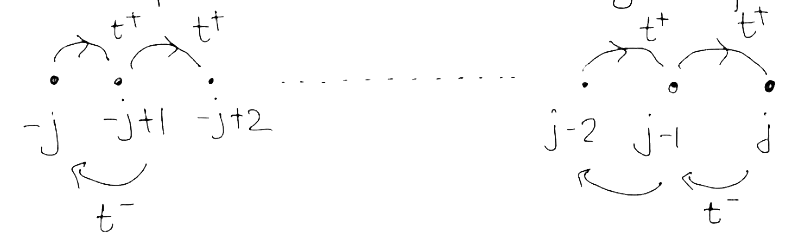
\includegraphics[width=0.6\linewidth]{24}
	\caption{}
	\label{fig:4}
\end{figure}
We said earlier that SU$(2)$ irreps are completely symmetric rank $r$ tensors since $r=2j+1$ is the dimensionality of the tensors.
\subsection{Strategy for representations: Roots and weights}
Recall that a Lie algebra is a set of generators with lie bracket commutators
\begin{equation}
	\begin{aligned}
		\left[X_a,X_b\right]=if_{abc}X_c
	\end{aligned}
\end{equation}
The lie bracket is antisymmetric and the $X_a$ are hermitian with $e^{iX_a}\in G$. The space of the generators is a vector space i.e. one can thing of the $X_a$'s as vectors. So one can in other words say that the Lie algebra is a vector space with additional structure provided by the Lie bracket.

The dimensionality of the vector space is given by the number of generators, so for SU(n) is a $n^2-1$ dimensional Lie algebra vector space, which we will denote by $\mathcal{L}$.

Remember for a representation we wanted to take our Lie algebra generators and think of them as linear operators in a vector space. If we take this vector space to be the Lie algebra itself, one gets the adjoint representation.
\subsubsection{Adjoint map}
The adjoint map takes two elements of the lie algebra and gives you a new element
\begin{equation}
	\begin{aligned}
		ad:~~y,x\in \mathcal{L}~~~~~~ad_y(x)=[x,y]
	\end{aligned}
\end{equation}
E.g. in SU(2)
\begin{equation}
	\begin{aligned}
		ad_{t_3}=[t_3,x], ~~~~x=\alpha_i t_i
	\end{aligned}
\end{equation}
One can think of the map $y\to ad_y$ as an association between $y\in \mathcal{L}$ and a linear operator. Since the commutator $[t_3,x]$ just gives a linear combination of the vectors making up the space.

We claim that $y\to ad_y$ provides a represenation. Read the lhs ad the lie algebra generator and the rhs as the operator representation which acts on a representation space $\mathcal{L}$. To confirm this we need to check
\begin{equation}
	\begin{aligned}
		\underbrace{\left[x,y\right]}_{\text{Lie bracket relation}}=z~~~~~~ \Rightarrow \underbrace{\left[ad_x,ad_y\right]}_{\text{Commutator of linear operators on } \mathcal{L}}=ad_z
	\end{aligned}
\end{equation}
If this claim is right we should be able to compute the bracket acting on a vector $w\in \mathcal{L}$
\begin{equation}
	\begin{aligned}
		\left[ad_x,ad_y\right]&=ad_x(ad_y(w))-ad_y(ad_x(w))\\
		&=ad_x(\left[y,w\right])-ad_y(\left[x,w\right])\\
		&=\left[x,\left[y,w\right]\right]-\left[y,\left[x,w\right]\right]\\
		&=-\left[w,\left[x,y\right]\right]~~~~~~~~~~~\text{ by Jacobi}\\
		&=ad_{[x,y]}(w)=ad_z(w)
	\end{aligned}
\end{equation}
Let us check this for SU(2)
\begin{equation}
	\begin{aligned}
		ad_{t_1}\begin{cases}
			t_1&=0\\
			t_2&=it_3\\
			t_3&=-it_2
		\end{cases},~~~~~~		ad_{t_2}\begin{cases}
		t_1&=-it_3\\
		t_2&=0\\
		t_3&=it_1
	\end{cases},~~~~~~		ad_{t_3}\begin{cases}
	t_1&=it_2\\
	t_2&-it_1\\
	t_3&=0
\end{cases}
	\end{aligned}
\end{equation}
So we can represent them as the matrices (after picking suitable basis vectors)
\begin{equation}
	\begin{aligned}
			ad_{t_1}:~\begin{pmatrix}
				0 & 0 & 0\\
				0 & 0 & i\\
				0 & -i & 0
			\end{pmatrix},~~~~
			ad_{t_2}:~\begin{pmatrix}
			0 & 0 & -i\\
			0 & 0 & 0\\
			i & 0 & 0
		\end{pmatrix},~~~~
	ad_{t_3}:~\begin{pmatrix}
	0 & i & 0\\
	-i & 0 & 0\\
	0 & 0 & 0
\end{pmatrix}
	\end{aligned}
\end{equation}
For SU(3) we have 8 generators, which in matrix from are the Gell-Mann matrices.
\begin{gather*}
	\lambda^1 = \matthree {0}{1}{0}{1}{0}{0}{0}{0}{0},\quad
	\lambda^2 = \matthree {0}{-i}{0}{i}{0}{0}{0}{0}{0},\quad
	\lambda^3 = \matthree {1}{0}{0}{0}{-1}{0}{0}{0}{0},\\[1ex]
	\lambda^4 = \matthree {0}{0}{1}{0}{0}{0}{1}{0}{0},\quad
	\lambda^5 = \matthree {0}{0}{-i}{0}{0}{0}{i}{0}{0},\quad
	\lambda^6 = \matthree {0}{0}{0}{0}{0}{1}{0}{1}{0},\\[1ex]
	\lambda^7 = \matthree {0}{0}{0}{0}{0}{-i}{0}{i}{0},\quad
	\lambda^8 = \frac{1}{\sqrt{3}} \matthree {1}{0}{0}{0}{1}{0}{0}{0}{-2}
\end{gather*}
One can split these into suitable lowering and raising pairs
\begin{equation}
	\begin{aligned}
		t_\pm=& \frac{1}{2}(\lambda_1\pm i\lambda_2)\\
		u_\pm=& \frac{1}{2}(\lambda_4\pm i\lambda_5)\\
			v_\pm=& \frac{1}{2}(\lambda_6\pm i\lambda_7)\\
			t_z=&\frac{1}{2}\lambda_3\\
			y=&\frac{1}{\sqrt{3}}\lambda_8
	\end{aligned}
\end{equation}
By computing matrix commutators we can get the $8\times 8$ adjoint representation.
So we have 8 generators and only two can be diagonalized simultaneously. Considering the eigenvalues of these, gives what is known as the weight. The raising and lowering operators then lower/raise this weight.
\subsection{Lie Algebras: Structure and representations}
Given a Lie algebra, find the maximal set of commuting generators, we denote this set by $\{H_i\}$ with $i=1,...,m$. These form a sub algebra, called the \textit{Cartan subalgebra}
\begin{equation}
	\begin{aligned}
		\left[H_i,H_j\right]=0
	\end{aligned}
\end{equation}
where $m$ is the rank of the Lie algebra. So if we try to find a representation on some vector space $V$, then we should diagonalize the $H_i$'s first. Label the states in $V$ by $H_i$ eigenvalues $\mu$ such that
\begin{equation}
	\begin{aligned}
		H_i\ket{\mu}=\mu_i\ket{\mu}
	\end{aligned}
\end{equation}
with $\ket{\mu}=\ket{\mu_1,\mu_2,\dots,\mu_m}$.We will refer to the $\mu$ as the weight vector, and the $\mu$'s themselves form a vectorspace, $\mu\in W$, with $W$: weight space.

Consider now the adjoint representation: states are specified by generators $t_a\to \ket{t_a}\in L$ 
\begin{itemize}
\item there are states of weight 0:
\begin{equation}
	\begin{aligned}
		H_i\ket{H_j}=0
	\end{aligned}
\end{equation}
from $[H_i,H_j]=0$ since the adjoint action is computing commutators.
\item Diagonalize rest of $L$ by combining generators into $\ket{E_\alpha}$
\begin{equation}
	\begin{aligned}
		H_i\ket{E_\alpha}=\alpha_i\ket{R_\alpha}
	\end{aligned}
\end{equation}
which means that $[H_i,E_\alpha]=\alpha_i E_\alpha$. Further, $E_\alpha$ is not hermitian  $[H_i,E_\alpha^\dagger]=-\alpha_i E_\alpha^\dagger$ and so $E_\alpha^\dagger=E_{-\alpha}$, meaning we have decomposed the lie algebra
\begin{equation}
	\begin{aligned}
		L&= \text{Cartan } \oplus \text{ Raising/lowering pairs}\\
		\oplus_{i}\{H_i\}\oplus_\alpha \{E_\alpha,E_{-\alpha}\}
	\end{aligned}
\end{equation}
\end{itemize}
The $\alpha_i$ are weights in adj rep and they are called the roots. We also define an inner product on $L$
\begin{equation}
	\begin{aligned}
		\braket{E_\alpha}{E_\beta}&=\frac{1}{\lambda}\Tr(E_\alpha^\dagger E_\beta)=\delta_{ab}\\
		\braket{H_i}{H_j}&=\frac{1}{\lambda}\Tr(H_i^\dagger h_j)=\delta_{ij}\\
	\end{aligned}
\end{equation}
Back to the general irrep
\begin{equation}
	\begin{aligned}
		H_i E_\alpha\ket{\mu}=[H_i,E_\alpha]\ket{\mu}+E_\alpha H_i\ket{\mu}=(\mu+\alpha)_i E_\alpha\ket{\mu}
	\end{aligned}
\end{equation}
So
\begin{equation}
	\begin{aligned}
		E_{\pm \alpha}\ket{\mu}=N_{\pm\alpha,\mu}\ket{\mu\pm\alpha}
	\end{aligned}
\end{equation}
The state $E_\alpha\ket{E_{-\alpha}}$ has weight 0 which means that it is a linear combination of the Cartan operators
\begin{equation}
	\begin{aligned}
		E_\alpha\ket{E_{-\alpha}}=\sum_{i=1}^{m}\beta _i\ket{H_i}
	\end{aligned}
\end{equation}
The commutation relations are 
\begin{equation}
	\begin{aligned}
		[H_i,H_j]=0,~~~~~[H_i,E_\alpha]=\alpha_i E_\alpha,~~~~~~ [E_\alpha,E_{-\alpha}]=\alpha_i H_i
	\end{aligned}
\end{equation}
The subalgebra satisfies: If L is a lie algbra and $M$ is a subset of L which is closed under the Lie bracket. The CArtan subalgebra is the maximal abelian subalgebra. An \textit{ideal} is a special subalgebra which projects all $J$
 such that if $x\in J, y\in L$ then $[x,y]\in J$. A Lie algebra with no ideals is said to be simple, and a Lie algebra with no Abelian ideals is semi-simple.

We will focus on semi-simple Lie algebras henceforth, for which $su(n)$ is an example.

We have seen that root vector are labels of Cartan eigenvalues in adj representation ($\alpha_i$'s). One can think of it in slightly different way. Consider the space of linear functionals acting on Cartan subalgebra. This is a dual vector space to the Cartan subvector space. Do if the Cartan vectors are kets, the functionals are the the bras. These functionals are called roots and the dual space is the root space.

The inner product on a Lie algebra is called the Killing form, denoted by $(\cdot,\cdot)$, so for $a,b\in L$ we define $(a,b)=\Tr[ad_a ad_b]$. Pick a basis for $L$ $\{x_i\}$ then 
\begin{equation}
	\begin{aligned}
		(a,b)(x)=ad_a ad_b(x_i)=[a,[b,x_i]]=\sum_j p_j x_j
	\end{aligned}
\end{equation}
If the killing form is nice, then we can map elements of Cartan and its dual (the root space)

Cartans theorem is: The Killing form is non degenerate if and only if $L$ is semi-simple.
\subsubsection{Example: SU(3)}
We have 8 generators and we have some combination of them, with the Cartan generators being $t_z$ and $y$. $x$ is part of the Cartan vector space $x=a t_z+b y$. 
\begin{equation}
	\begin{aligned}
		H=\text{span}\{t_z,y\}
	\end{aligned}
\end{equation}
with the killing form computed by the adjoint action
\begin{equation}
	\begin{aligned}
		(t_z,t_z)=&3\\
		(y,y)=&4\\
		(t_+,t_-)=&(u_+,u_-)=(v_+,v_-)=6
	\end{aligned}
\end{equation}
If we look at the dual space $H^*$: We want to understand this space and find a useful basis. We will view $H^*$ as a real vector space and say that if $\alpha,\beta \in H^*$ then these are associated to the following vectors in the Cartan space $h_\alpha,h_\beta\in H$.

There is an inner product on the dual space using the Killing form in the Cartan vector space
\begin{equation}
	\begin{aligned}
		\langle\alpha ,\beta \rangle=(h_\alpha,h_\beta)
	\end{aligned}
\end{equation}

As described $at_z+by\in H$. If we denote our root vector by $\alpha_1,\alpha_2,\alpha_3\in H^*$, with
\begin{equation}
	\begin{aligned}
		\alpha_1(at_z+by)&=a,~~~~~~\alpha_1\leftrightarrow t_+ \\
		\alpha_2(at_z+by)&=-a/2+b,~~~~~~\alpha_2\leftrightarrow u_+ \\
		\alpha_3(at_z+by)&=a/2+b,~~~~~~\alpha_3\leftrightarrow v_+ 
	\end{aligned}
\end{equation} 
So the rootvectors are linear functionals that act on cartan vectors and give back numbers. Let us find the associated Cartan vector combinations $h_{\alpha_1},h_{\alpha_2},h_{\alpha_3}$:
\begin{equation}
	\begin{aligned}
		h_{\alpha_i}=(c_it_z+d_i y)
	\end{aligned}
\end{equation}
so 
\begin{equation}
	\begin{aligned}
		\alpha_1(t_z)=(h_{\alpha_1},t_z)=(c_1 t_z, d_1+y, t_z)&=3c_1
		\alpha_1(y)=(h_{\alpha_1},y)=(c_1 t_z, d_1+y, y)=4d_1
	\end{aligned}
\end{equation}
and we get $h_{\alpha_1}=\frac{1}{3}t_z$ and similarly for the other $h$'s. Using them we can then find $\langle\alpha_i,\alpha_j\rangle=(h_{\alpha_i},h_{\alpha_j})$.
\subsection{Structure of Lie algbera}
The Lie algebra can be decomposed $L=H\cup R$ where $R$ is the set of all roots.
%%%%%%%%%%%%%%%%%%%%%%%%%%%%%%%%%%%%%%%%%%%%%%%%%%%%%%%%%%%%%%%%%%%%%%%%%%%%%%%%%%%%%%%%%%%%%%%%%%%%%%%%%%%%%%%%%%%%%%%%%%%%%%%%%%%%%%%%%%%%%%
\newpage
\section*{Homework 1\\\\
Taro V. Brown}\vspace*{1cm}
\section*{Problem 1}
\subsection*{Part a}
We compute
\begin{equation}
\oint_{|z|=3} \dd z\frac{4z-3}{z(z-2)}
\end{equation}
Inside the contour this has poles at $z=0$ and $z=2$ so using 
\begin{equation}
	\oint _C \dd z  f(z)=2\pi i \sum_{a_i\in D}\Res[f(a_i)]
\end{equation}
We get
\begin{equation}
\begin{aligned}
	\oint_{|z|=3} \dd z\frac{4z-3}{z(z-2)}=&2\pi i \left\{\Res[\frac{4z-3}{z(z-2)}]_{z=0}+\Res[\frac{4z-3}{z(z-2)}]_{z=2}\right\}\\
	=&2\pi i \left\{\frac{4\times 0-3}{(0-2)}+\frac{4\times 2-3}{2}\right\}\\
	=&2\pi i \left\{\frac{3}{2}+\frac{5}{2}\right\}\\	
	=&8\pi i 
\end{aligned}
\end{equation}
\subsection*{Part b}
Similarly
\begin{equation}
	\begin{aligned}
		\oint_{|z|=3} \dd z\frac{e^z}{(z-1)(z-2)}=&2\pi i \left\{\Res[\frac{e^z}{(z-1)(z-2)}]_{z=1}+\Res[\frac{e^z}{(z-1)(z-2)}]_{z=2}\right\}\\
		=&2\pi i \left\{-e+e^2\right\}\\
	\end{aligned}
\end{equation}
\section*{Problem 2}
\subsection*{Part a}
Computing
\begin{equation}
	\begin{aligned}
		\int_{0}^{\infty}\dd x\frac{2x^2-1}{x^6+1}
		=&	\frac{1}{2}\int_{-\infty}^{\infty}\dd x\frac{2x^2-1}{x^6+1}
		\\
		=&\frac{1}{2}\oint_{|z|=2} \dd z\frac{2z^2-1}{z^6+1}
	\end{aligned}
\end{equation}
$z^6+1$ has zero's within the contour at $z=\{i,(-1)^{\frac{1}{6}},(-1)^{\frac{5}{6}}\}$ and the residues can be computed by first factoring out the denominator 
\begin{equation}
(x^6+1)=(x-i)(x+i)\left(x-(-1)^{\frac{1}{6}}\right)\left(x+(-1)^{\frac{1}{6}}\right)\left(x-(-1)^{\frac{5}{6}}\right)\left(x+(-1)^{\frac{5}{6}}\right)
\end{equation}
and then applying the usual trick for first order poles. We get
\begin{equation}
\begin{aligned}
		\\
		=&\pi i
		 \left\{\Res[\frac{2z^2-1}{z^6+1}]_{z=i}+\Res[\frac{2z^2-1}{z^6+1}]_{z=(-1)^{\frac{1}{6}}}+\Res[\frac{2z^2-1}{z^6+1}]_{z=(-1)^{\frac{5}{6}}}\right\}\\
		=&\pi i \left\{\frac{i}{2}+\frac{1}{6}\left(-2i+(-1)^{\frac{1}{6}}\right)+\frac{1}{6}\left(-2i+(-1)^{\frac{5}{6}}\right)\right\}\\
		&=0
	\end{aligned}
\end{equation}

\subsection*{Part b}
For this integral we will be using $\sin n\theta =\frac{1}{2i}\left(z^n-z^{-n}\right)$, $\cos n\theta =\frac{1}{2}\left(z^n+z^{-n}\right)$ and $\dd \theta=\frac{1}{iz}\dd z$. We choose the contour $|z|=1$ since this includes all poles that show up. Computing we find
\begin{equation}
	\begin{aligned}
		\int_{0}^{\pi}\dd x\frac{\cos^2(3x)}{5-4\cos(2x)}
		=&\oint_{|z|=1}\frac{\dd z}{iz}\frac{\left(z^3+\frac{1}{z^3}\right)^2}{4 \left(1-2 \left(z^2+\frac{1}{z^2}\right)\right)}\\
		=&\oint_{|z|=1}\dd z \frac{i \left(z^6+1\right)^2}{8 z^9-4 z^7+8 z^5}\\
			=&2\pi i \left\{
			\Res[\frac{\left(z^6+1\right)^2}{8 z^9-4 z^7+8 z^5}]_{z=0}
			\right\}\\
			=&\frac{3\pi}{16}
	\end{aligned}
\end{equation}
\subsection*{Part c}
The following integral is a little tricky. First we rewrite the outer cosine at the real part of a complex function and combine the exponentials
\begin{equation}
\begin{aligned}
\int_{0}^{\pi}\dd x\, e^{\cos(x)}\cos[nx-i\sin(x)]&=\frac{1}{2}\Re\left[\int_{-\pi}^{\pi}\dd x\, e^{\cos(x)+inx-i\sin(x)}\right]\\
&=\frac{1}{2}\Re\left[\int_{-\pi}^{\pi}\dd x\, e^{inx}e^{e^{-ix}}\right]
\end{aligned}
\end{equation}
where we have used $e^{-ix}=\cos(x)-i\sin(x)$. Now
substituting $z=e^{-ix}$, which leads to $\dd z=-i e^{-ix} \dd x=-iz \dd x$
%%%%%%%%%%%%%%%%%%%%%%%%%%%%%%%%%%%%%%%%%%%%%%%%%%%%
\begin{equation}
	\begin{aligned}
\int_{0}^{\pi}\dd x\, e^{\cos(x)}\cos[nx-\sin(x)]&=\frac{1}{2}\Re\left[\int_{-\pi}^{\pi}\dd z\, \frac{e^{z}}{z^{(n+1)}}\right]\\
&=\frac{1}{2}\Re\left[\oint_{|z|=1}-i\dd z\, \frac{e^{z}}{z^{(n+1)}}\right]\\
	\end{aligned}
\end{equation}
This has an $n$'th order pole at $z=0$. We can find the residues using
\begin{equation}
	\Res[f(z=a)]=\frac{1}{(m-1)!}\lim_{z\to a}\dv[m-1]{}{z}[(z-a)^mf(z)]
\end{equation}
which in this case is particularly easy since we have an exponential function, so
\begin{equation}
	\begin{aligned}
		\int_{0}^{\pi}\dd x\, e^{\cos(x)}\cos[nx-\sin(x)]&=
		\Re\left [\pi \Res[\frac{e^{z}}{z^{(n+1)}}]_{z=0}\right]\\
		&=\frac{\pi}{n!}
	\end{aligned}
\end{equation}
\subsection*{Part d and Part e}
Lastly we have the two $\sinh$ integrals, with different contours. Let us first note that we have the Laurent series:
\begin{equation}
\frac{1}{\sinh z}=\frac{1}{z}-\frac{1}{6}z^2+\frac{7}{16}z^3+\cdots
\end{equation}
so that the combination
\begin{equation} \label{eq:sinh}
	\frac{1}{z^2\sinh z}=\frac{1}{z^3}-\frac{1}{6z}+\frac{7}{16}z+\cdots
\end{equation}
Further, we know that the zeroes of $\sinh z$ are at $n\pi i $, $n\in\mathds{Z}$ while for $z^2$ it is at $0$. This means that we for the contour $|z|=1$ only have to take the residue at $z=0$, while for $|z|=4$ also have to include the residue at $z=i\pi$. \eqref{eq:sinh} has a third order pole and a first order pole however since calculating the residue of the third order pole requires differentiating twice it's residue is just zero and we only need the contribution from the first order pole
\begin{equation}
\begin{aligned}
\oint_{|z|=1}\dd z\,\frac{1}{z^2\sinh z}  &=2\pi i \Res[\frac{1}{z^2\sinh z}]_{z=0}\\
&=2\pi i \left[-\frac{1}{6}\right]\\
&=-\frac{\pi i}{3}
\end{aligned}
\end{equation}
For the larger contour we, as mentioned, have to include the residue at $i\pi$ and $-i\pi$. The residue at this point be calculated using
\begin{equation}
\Res[\frac{p(z)}{q(z)}]_{z=a}=\lim_{z\to a}\left[\frac{p(z)}{q'(z)}\right]
\end{equation}
where $q(z)$ has a pole at $z=a$ and $p(z)$ does not. Hence taking $q(z)=\sinh(z)$ and $p(z)=z^2$  we have
\begin{equation}
\begin{aligned}
\Res[\frac{1}{z^2}\frac{1}{\sinh z}]_{z=i \pi}&=\lim_{z\to i\pi }\left[\frac{1}{z^2}\frac{1}{\cosh z}\right]\\
&=\frac{1}{\pi^2}
\end{aligned}
\end{equation}
and
\begin{equation}
	\begin{aligned}
		\Res[\frac{1}{z^2}\frac{1}{\sinh z}]_{z=-i \pi}&=\lim_{z\to -i\pi }\left[\frac{1}{z^2}\frac{1}{\cosh z}\right]\\
		&=\frac{1}{\pi^2}
	\end{aligned}
\end{equation}
So the total contour integral is
\begin{equation}
	\begin{aligned}
		\oint_{|z|=4}\dd z\,\frac{1}{z^2\sinh z}  &=2\pi i \left\{
		\Res[\frac{1}{z^2\sinh z}]_{z=0}+\Res[\frac{1}{z^2\sinh z}]_{z=i\pi}+\Res[\frac{1}{z^2\sinh z}]_{z=-i\pi}
		\right\}\\
		&=2\pi i \left[-\frac{1}{6}+\frac{1}{\pi^2}+\frac{1}{\pi^2}\right]\\
		&=2\pi i \left[-\frac{1}{6}+\frac{2}{\pi^2}\right]
	\end{aligned}
\end{equation}
\section*{Problem 3}
Using Cauchy's integral formula
\begin{equation}
	\begin{aligned}
f(a)&=\frac{1}{2\pi i}\oint_{z=|R|} \dd z\,\frac{f(z)}{z-a}
	\end{aligned}
\end{equation}
We can subtract the following term since it is zero inside this contour by Cauchy's theorem
\begin{equation}
	\begin{aligned}
		0&=\frac{1}{2\pi i}\oint_{z=|R|} \dd z\,\frac{f(z)\bar a}{ R^2-\bar az}
	\end{aligned}
\end{equation}
So we get
\begin{equation}
	\begin{aligned}
		f(a)&=\frac{1}{2\pi i}\oint_{z=|R|} \dd z\,\left[\frac{f(z)}{z-a}-\frac{f(z)\bar a}{ R^2-\bar az}\right]\\
		&=\frac{1}{2\pi i}\oint_{z=|R|} \dd z\,f(z)\frac{R^2-\bar a a}{(z-a)(R^2-\bar az)}\\
	\end{aligned}
\end{equation}
Where we have put everything on a common denominator in the last term. Expanding this denominator and writing $|a|^2=\bar a a$ we find
\begin{equation}
	\begin{aligned}
		f(a)
		&=\frac{1}{2\pi i}\oint_{z=|R|} \frac{\dd z}{z}\,f(z)\frac{R^2-|a|^2}{R^2-2\Re(a\bar z)+|a|^2}
	\end{aligned}
\end{equation}
Then letting $a=re^{i\theta}$ and integrating around the contour by setting $z=Re^{i\phi}$, $0\leq \phi \leq 2\pi$ \footnote{Note that we in the above have used $\bar z=z^{-1}$}. Further we have $\dd z=iRe^{i\phi}\dd \phi=iz\dd \phi$ and $|a|^2=r^2$, then
\begin{equation}
	\begin{aligned}
f(re^{i\theta})&=\frac{1}{2\pi i}\int_{0}^{2\pi} \dd \phi\,f(Re^{i\phi})\frac{R^2-r^2}{R^2-2Rr\cos(\theta-\phi)+r^2}
	\end{aligned}
\end{equation}
Since $f$ was assumed analytic inside the disc, this solves the Laplace equation in this region since it can be written in terms of harmonic functions through the Cauchy-Riemann conditions.
\section*{Problem 4}
\subsection*{Part a}
We have the Navier-Stokes equation:
\begin{equation}
\partial_t \bm u+\bm u\cdot  \nabla\bm u=-\nabla \left(\frac{1}{\rho} p- V\right)+\nu\nabla^2 \bm u
\end{equation}
Taking the curl on both sides we use the fact that the curl of a gradient of scalar is zero 
\begin{equation} \label{eq:ns}
	\partial_t \bm \omega+\nabla\times(\bm u \cdot \nabla\bm u)=+\nu\nabla^2 \bm w
\end{equation}
Furtherm, since $\nu=0$ in this case
\begin{equation} \label{eq:ns}
	\partial_t \bm \omega+\nabla\times(\bm u \cdot \nabla\bm u)=0
\end{equation}
Then using the fact that
\begin{equation}
\bm u \cdot \nabla\bm u=\frac{1}{2}\nabla u^2-\bm u\times (\nabla \times \bm u)=\frac{1}{2}\nabla u^2-\bm u\times \bm \omega
\end{equation}
we can rewrite
\begin{equation}
\begin{aligned}
\nabla\times(\bm u \cdot \nabla\bm u)&=\frac{1}{2}\nabla\times\nabla u^2-\nabla\times (\bm u\times \bm \omega)\\
&=\nabla\times (\bm \omega \times \bm u)\\
&=(\bm u \cdot \nabla)\bm\omega -(\bm \omega  \cdot \nabla)\bm u +\bm\omega (\nabla\cdot \bm u)+\bm u (\nabla\cdot \bm \omega )\\
&=(\bm u \cdot \nabla)\bm\omega -(\bm \omega  \cdot \nabla)\bm u
\end{aligned}
\end{equation}
where the we have used $\nabla\cdot \bm u=0$ and $\bm u(\nabla \cdot \bm \omega)=\bm u(\nabla \cdot (\nabla \times \bm u))=0$ in the third line. Inserting this back into \ref{eq:ns}:
\begin{equation} \label{eq:ns2}
	\partial_t \bm \omega+(\bm u \cdot \nabla)\bm\omega =(\bm \omega  \cdot \nabla)\bm u
\end{equation}
Or in index notation:
\begin{equation} \label{eq:ns2}
	\partial_t \omega_i+ u ^j \partial_j\omega_i = \omega^j  \partial_j u_i
\end{equation}
\subsection*{Part b}
If $\bm \omega =\nabla\times \bm u =0$, we could write
\begin{equation}
\bm u=\nabla \phi
\end{equation}
Since the equation
\begin{equation}
\nabla\times \nabla\phi =0
\end{equation}
is automatically satisfied. This is similar to the gauge potential in electrodynamics. Further from the incompressibility we know $\phi$ satisfies the Laplace equation
\begin{equation}
\nabla\cdot u=\nabla^2 \phi=0
\end{equation}
\subsection*{Part c}
First we insert $u=\nabla\phi$ into Navier-Stokes equation. Note that the following terms can be rewritten as:
\begin{equation}
\begin{aligned}
\bm u \cdot \nabla\bm u&=\frac{1}{2}\nabla u^2-\bm u\times (\nabla \times \bm u)\\
&=\frac{1}{2}\nabla u^2-\bm u\times (\nabla \times \nabla\phi)\\
&=\frac{1}{2}\nabla u^2
\end{aligned}
\end{equation}
So that we after inserting get:
\begin{equation}
	\nabla \partial_t \phi+ \frac{1}{2}\nabla \phi^2+=-\nabla \left(\frac{1}{\rho} p+ V\right)
\end{equation}
Which we can write as
\begin{equation}
	\nabla \left(\partial_t \phi+\frac{1}{2} u^2+\frac{p}{\rho} + V\right)=0
\end{equation}
This means that we can write the part in parenthesis as a constant in space but function of time $F(t)$
\begin{equation}
 \left(\partial_t \phi+\frac{1}{2} u^2+\frac{p}{\rho} + V\right)=F(t)
\end{equation}
Finally since we can just absorb the time-dependence through a shift in $\phi(t)\to\phi'$ we can write this as
\begin{equation} \label{eq:flow}
\partial_t \phi'+\frac{1}{2} u^2+\frac{p}{\rho} + V=0
\end{equation}
\subsection*{Part d}
We have already shown that since we have irrotational flow, i.e. $\nabla\times \bm u=0$ we can write the flow field as a gradient
\begin{equation}
\begin{aligned}
	u_x&=\partial_x \phi\\
	u_y&=\partial_y \phi
\end{aligned}
\end{equation}
Further, since we have an incompressible fluid, i.e. $\nabla\cdot\bm  u=0$ we can write it as a "curl" of a scalar\footnote{Since there doesn't exist such thing as a curl of scalar function, the use of curl in this case should be taken as meaning \begin{equation}
\bm u=\nabla\times \begin{pmatrix}
1\\1
\end{pmatrix}\chi
\end{equation}}
\begin{equation}
\begin{aligned}
u_x&=\partial_y \chi\\
u_y&=-\partial_x \chi
\end{aligned}
\end{equation}
since it automatically satisfies $\nabla\cdot u=0$. We see that in this case we can use either $\phi$ or $\chi$ to solve \eqref{eq:flow} and that further
\begin{equation}
	\begin{aligned}
		\partial_x \phi&=\partial_y \chi\\
		\partial_y \phi&=-\partial_x \chi
	\end{aligned}
\end{equation}
These are just the Cauchy-Riemann relations and so we we can construct an analytic function out of these, known as the stream function
\begin{equation}
\Phi=\phi+i\chi
\end{equation}
This stream-function also solves \eqref{eq:flow} since the derivatives act linearly on it as a consequence of the Cauchy-Riemann relations. This can be seen by multiplying the two sides
\begin{equation}
-\partial_x\phi\partial_x\chi=\partial_y\phi\partial_y\chi
\end{equation}
implying $(\nabla\phi)\cdot (\nabla\chi)=0$. This also implies that $\phi$ is tangent to the level sets of $\chi$. As mentioned, the terms with derivatives on $\Phi$ then become linear combinations of $\phi$ and $\chi$ and so $\Phi$ must solve the equation as well:
\begin{equation}
|\nabla \Phi|^2=(\nabla \phi+i\nabla\chi)(\nabla \phi-i\nabla\chi)=(\nabla\phi)^2+(\nabla\chi)^2
\end{equation}
\subsection*{Part e}
Here we refer to the Milne-Thomson theorem which can be used to obtain the stream-function in the case of a cylindrical obstacle through
\begin{equation}
\tilde \Phi=\Phi(z)+\bar \Phi\left(\frac{a^2}{z}\right)
\end{equation}
In this case we will assume a uniform flow with speed $u=\frac{1}{2}$ in the $x$-direction and so we have the stream-line function $\Phi(z)=\frac{1}{2}z$ and place the cylinder with $a=1$, so we get 
\begin{equation}
	\begin{aligned}
	\tilde \Phi&= \frac{1}{2}\left(z+\frac{1}{z}\right)
	\end{aligned}
\end{equation}
On the curve $|z|=1$, we have $\bar z = \frac{1}{z}$ and so the imaginary part of $\Phi$ is zero. Since $\chi=constant$ represented the constant flow streamlines, the surface of the cylinder has become a streamline and the flow doesn't penetrate this surface. This also means that the solutions holds for $|z|>1$ as prescribed in the problem.
%%%%%%%%%%%%%%%%%%%%%%%%%%%%%%%%%%%%%%%%%%%%%%%%%%
\newpage
\section*{Homework 2\\\\
	Taro V. Brown}\vspace*{1cm}
\section*{Problem 1}
\subsection*{Part a}
We will use the map provided in class
\begin{equation}
z=\frac{a}{\pi}(1+w+e^w)
\end{equation}
which maps a pair of infinite lines in the $w$ plane to a pair of semi-infinite lines in the $z$ plane. Note that the normalization in front makes sure the capacitors go from being at $a,-a$ to $-\pi,\pi$. We will analyze the lines  $w=u\pm iv$, since the equipotentials are straight lines. Inserting into the transformation:
\begin{equation}
\begin{aligned}
	z(u+iv)&=\frac{a}{\pi}(1+u+iv+e^{u+iv})\\
	&=\frac{a}{\pi}(1+u+iv+e^{u}\left[\cos v+i\sin v\right])
	\\
	&=\frac{a}{\pi}(\left[1+u+e^{u}\cos v\right]+i\left[v+e^{u}\sin v\right])
\end{aligned}
\end{equation}
From which we can identify $x$ and $y$ by setting $z=x+iy$, so
\begin{equation}
\begin{aligned}
	x&=\frac{a}{\pi}\left[1+u+e^{u}\cos v\right]\\
	y&=\frac{a}{\pi}\left[v+e^{u}\sin v\right]
\end{aligned}
\end{equation}
The potential in the infinite capacitor is $V\sim V_0v$ between the places. This potential is the imaginary part of the analytic function $\Phi(w)\sim V_0 w$. This means that varying $u$ at constant some constant $v$ will give the the equipotential lines and similarly varying $v$ at constant $u$ values give the electric field lines. We now provide a sketch of this as well as the Mathematica code written to do so. We have chosen $a=\pi$ for convenience.
\begin{lstlisting}
Potential = 
ParametricPlot[{{1 + u + Exp[u] Cos[Pi / 6], 
		Pi / 6 + Exp[u] Sin[Pi / 6]}, {1 + u + Exp[u], 
		0}, {1 + u + Exp[u] Cos[Pi / 3], 
		Pi / 3 + Exp[u] Sin[Pi / 3]}, {1 + u + Exp[u] 
		Cos[Pi / 2], 
		Pi / 2 + Exp[u] Sin[Pi / 2]}, {1 + u + Exp[u]
		Cos[2 Pi / 3], 
		2 Pi / 3 + Exp[u] Sin[2 Pi / 3]}, {1 + u + Exp[u] 
		Cos[5 Pi / 6], 
		5 Pi / 6 + Exp[u] Sin[5 Pi / 6]}, {1 + u + Exp[u] 
		Cos[8 Pi / 9], 
		8 Pi / 9 + Exp[u] Sin[8 Pi / 9]}, {1 + u + Exp[u] 
		Cos[0.97 Pi], 
		0.97 Pi + Exp[u] Sin[0.97 Pi]},
	{1 + u + Exp[u] Cos[-Pi / 6], -Pi / 6 + Exp[u] 
		Sin[-Pi / 6]}, {1 +
		u + Exp[u], 
		0}, {1 + u + Exp[u] Cos[-Pi / 3], -Pi / 3 + 
		Exp[u] Sin[-Pi / 3]}, {1 + u + Exp[u] 
		Cos[-Pi / 2], -Pi / 2 + 
		Exp[u] Sin[-Pi / 2]}, {1 + u + 
		Exp[u] Cos[-2 Pi / 3], -2 Pi / 3 + Exp[u] 
		Sin[-2 Pi / 3]}, {1 + 
		u + Exp[u] Cos[-5 Pi / 6], -5 Pi / 6 + 
		Exp[u] Sin[-5 Pi / 6]}, {1 + u + 
		Exp[u] Cos[-8 Pi / 9], -8 Pi / 9 + Exp[u] 
		Sin[-8 Pi / 9]}, {1 + 
		u + Exp[u] Cos[-0.97 Pi], -0.97 Pi + 
		Exp[u] Sin[-0.97 Pi]}}, {u, -9, 2.43}, 
PlotStyle -> {{Gray, Thick}, {Gray, Thick}}];
Plates = ParametricPlot[{{1 + u + Exp[u] Cos[Pi], 
		Pi + Exp[u] Sin[Pi]}, {1 + u + Exp[u] 
		Cos[-Pi], -Pi + 
		Exp[u] Sin[-Pi]}}, {u, -9, 2.43}, 
PlotStyle -> {{Blue, Thick}, {Blue, Thick}}];
Electric = 
ParametricPlot[{{1 + -8. + Exp[-8] Cos[v], 
		v + Exp[-8] Sin[v]}, {1 + -6. + Exp[-6] Cos[v], 
		v + Exp[-6] Sin[v]}, {1 + -4 + Exp[-4] Cos[v], 
		v + Exp[-4] Sin[v]}, {1 + -2 + Exp[-2] Cos[v], 
		v + Exp[-2] Sin[v]}, {1 + -1 + Exp[-1] Cos[v], 
		v + Exp[-1] Sin[v]}, {1 + 0 + Exp[0] Cos[v], 
		v + Exp[0] Sin[v]}, {1 + 1 + Exp[1] Cos[v], 
		v + Exp[1] Sin[v]}, {1 + 2 + Exp[2] Cos[v], 
		v + Exp[2] Sin[v]}, {1 + 1.5 + Exp[1.5] Cos[v], 
		v + Exp[1.5] Sin[v]}}, {v, -\[Pi], Pi}, 
PlotStyle -> {{Red, Dashed}, {Red, Dashed}}];
Show[Electric, Plates, Potential]
\end{lstlisting}
Which results in the following figure
\begin{figure}[H]
	\centering
	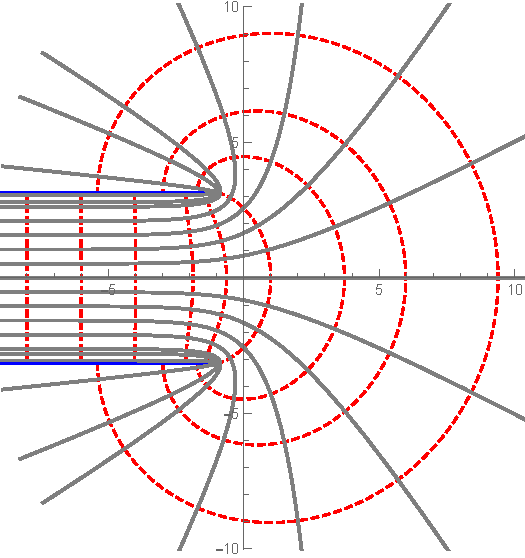
\includegraphics[width=0.7\linewidth]{hw2.pdf}
	\caption{Plot of equipotential lines (grey) and field lines (red, dashed)}
	\label{fig:4}
\end{figure}
%%%%%%%%%%%%%%%%%%%%%%%%%%%%%%%%%%%%%%%%%%%%%%%%%%
%%%%%%%%%%%%%%%%%%%%%%%%%%%%%%%%%%%%%%%%%%%%%%%%%%
%%%%%%%%%%%%%%%%%%%%%%%%%%%%%%%%%%%%%%%%%%%%%%%%%%
\subsection*{Part b}
We will here use the following map, obtained from the conformal dictionary
\begin{equation}
w=\frac{2}{\pi}\asin(z)
\end{equation}
This maps two lines to two parallel plates. The inverse, which is the one we are interested in, is
\begin{equation}
	z=\sin(\frac{2}{\pi}w)
\end{equation}
First we write it in terms of its real and complex parts using a trig identity
\begin{equation}
\begin{aligned}
	x+iy=z=\sin((u+iv)\frac{2}{\pi})=\sin\frac{\pi}{2}u\cosh\frac{\pi}{2}v+i\cos\frac{\pi}{2}u\sinh\frac{\pi}{2}v
\end{aligned}
\end{equation}
Then to find equipotentials we first identity
\begin{equation}
\begin{aligned}
x&=\sin\frac{\pi}{2}u\cosh\frac{\pi}{2}v\\
y&=\cos\frac{\pi}{2}u\sinh\frac{\pi}{2}v
\end{aligned}
\end{equation}
Then taking $u=constant$ we get
\begin{equation}
	\begin{aligned}
		\left(\frac{x}{\sin\frac{\pi}{2}u}\right)^2-\left(\frac{y}{\cos\frac{\pi}{2}u}\right)^2=\cosh^2\frac{\pi v}{2}-\sinh^2\frac{\pi v}{2}=1
	\end{aligned}
\end{equation}
or a hyperbola. Smiliar holding $v$ constant to find the field lines, we get elipses
\begin{equation}
	\begin{aligned}
		\left(\frac{x}{\cosh\frac{\pi}{2}v}\right)^2+\left(\frac{y}{\sinh\frac{\pi}{2}v}\right)^2=\cos^2\frac{\pi u}{2}+\sin^2\frac{\pi u}{2}=1
	\end{aligned}
\end{equation}
Both hyperboles and elipses are conic sections. Sketching these for different values of $u$ and $v$ we get, using the following mathematica code
\begin{lstlisting}
ContourPlot[{x^2/Sin[1]^2 - y^2/Cos[1]^2 == 1, 
	x^2/Sin[2]^2 - y^2/Cos[2]^2 == 1, 
	x^2/Sin[2.5]^2 - y^2/Cos[2.5]^2 == 1, 
	x^2/Sin[3]^2 - y^2/Cos[3]^2 == 1, 
	x^2/Cosh[1]^2 + y^2/Sinh[1]^2 == 1, 
	x^2/Cosh[2]^2 + y^2/Sinh[2]^2 == 1, 
	x^2/Cosh[2.5]^2 + y^2/Sinh[2.5]^2 == 1, 
	x^2/Cosh[3]^2 + y^2/Sinh[3]^2 == 1},
 	{x, -6.5, 6.5}, {y, -6.5, 6.5}]
\end{lstlisting}
\begin{figure}[H]
	\centering
	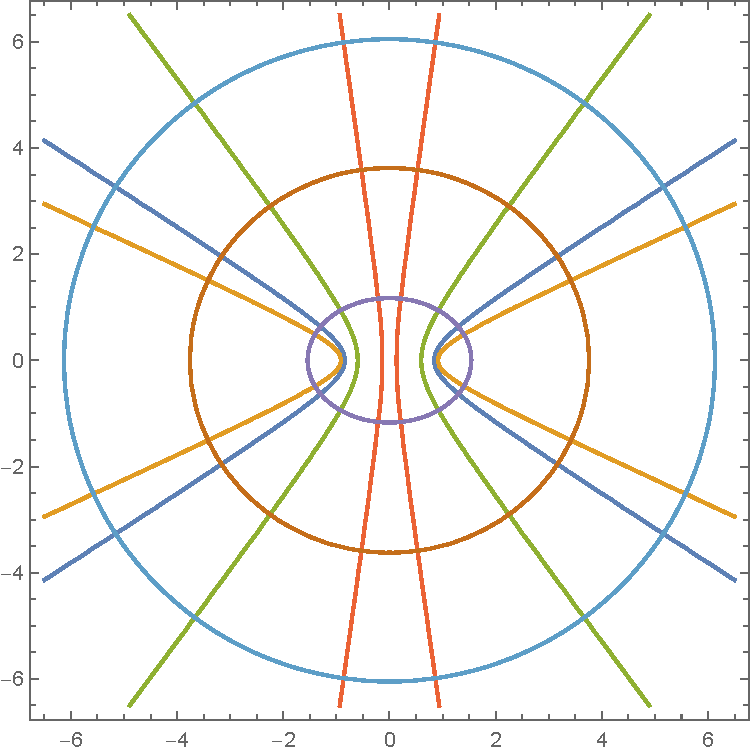
\includegraphics[width=0.7\linewidth]{contour.pdf}
	\caption{Plot of equipotential lines (parabolas) and field lines (elipses)}
	\label{fig:4}
\end{figure}
\section*{Problem 2}
The transformation that takes the unit disc to the unit disc is the linear fractional transformation
\begin{equation}
f(z)= e^{i\phi}\frac{z-\alpha}{\bar \alpha z-1},~~~~~~|\alpha|<1,~~~~~-\pi<\phi < \pi
\end{equation}
The rotation part $e^{i\phi}$ obviously just maps points in the disc to other points in the disc, while the linear fraction part moves the origin from $z=0$ to $f=\alpha$. We can show that this maps to the unit disc if $|f(z)|<1$ so that every point in the domain lies within the disc. First we note that
\begin{equation}
\begin{aligned}
|z-a|^2&=(z-a)(\bar z-\bar a)=|z|^2+|\alpha|^2-\alpha \bar z-\bar \alpha z\\
|\bar \alpha z-1|^2&=(\bar \alpha z-1)( \alpha \bar z-1)=|z|^2|\alpha|^2-\alpha \bar z-\bar \alpha z+1
\end{aligned}
\end{equation}
If we take the difference of the two we find
\begin{equation}
\begin{aligned}
|z-a|^2-|\bar \alpha z-1|^2&=|z|^2+|\alpha|^2-\alpha \bar z-\bar \alpha z-|z|^2|\alpha|^2+\alpha \bar z+\bar \alpha z-1\\
&=|z|^2+|\alpha|^2-|z|^2|\alpha|^2-1\\
&<0
\end{aligned}
\end{equation}
where the last inequality only holds since we started within the disc, $|z|<1$, and since we assumed $|\alpha|<1$. This implies that $|z-a|<|\bar \alpha z-1|$ and hence that 
\begin{equation}
\begin{aligned}
|f(z)|=\frac{|z-\alpha|}{|\bar \alpha z-1|}<1
\end{aligned}
\end{equation}
which means that every point in the new domain, lies within the unit circle.  
\section*{Problem 3}
\subsection*{Part a}
Here we will use the composition law
\begin{itemize}
	\item If $w=f(z)$ and $\zeta=g(w)$ are analytic then $\zeta= g\circ f(z)$ is a conformal map from $z\to \zeta$ planes
\end{itemize}
First we will use the following map presented in class, namely
\begin{equation}
w=\frac{z+1}{z-1}
\end{equation}
which maps the half disc $z\in D_+$ to the upper right quadrant (URQ) $w\in 0<\arg w <\frac{1}{2}\pi$. The map that takes the URQ to the unit disc is found in the conformal dictionary
\begin{equation}
 \zeta(w)=\frac{iw^2+1}{iw^2-1}
\end{equation}
Taking the composition we find
\begin{equation}
\begin{aligned}
\zeta(w=\frac{z+1}{z-1})&=\frac{i\left(\frac{z+1}{z-1}\right)^2+1}{i\left(\frac{z+1}{z-1}\right)^2-1}\\
&=\frac{-i\left(1+2iz+z^2\right)}{1-2iz+z^2}
\end{aligned}
\end{equation}
The factor $-i$ in front is the same as rotating the disc, which also leaves it invariant so a valid solution is also
\begin{equation}
	\begin{aligned}
		\zeta(z)
		&=\frac{\left(1+2iz+z^2\right)}{1-2iz+z^2}
	\end{aligned}
\end{equation}
Note that this can also be simplified to
\begin{equation}
	\begin{aligned}
		\zeta(z)
		&=1+\frac{4iz}{1-2iz+z^2}
	\end{aligned}
\end{equation}
though the fractional form might be nicer to use. One can further note that this map is not unique and by acting with the transformation found in the previous problem the disc would still be invariant and hence one could use the composition with this, to map the half disc at the origin to the unit disc centered around a different origin:
\begin{equation}
	\begin{aligned}
		\zeta 
		&=e^{i\phi}\frac{\left(1+\frac{4iz}{1-2iz+z^2}\right)-\alpha}{\bar \alpha \left(1+\frac{4iz}{1-2iz+z^2}\right)-1}\\
		&=e^{i\phi}\frac{\left(1+2iz+z^2\right)-\alpha(1-2iz+z^2)}{-1+\bar a+2i(1+\bar a)z+(-1+\bar a)z^2}
		\\
		&=e^{i\phi}\frac{\left(1+2iz+z^2\right)-\alpha(1-2iz+z^2)}{\alpha(1+2iz+z^2)-\left(1-2iz+z^2\right)},~~~~~~|\alpha|<1,~~~~~-\pi<\phi < \pi
	\end{aligned}
\end{equation}
\subsection*{Part b}
We will assume the radius of the outer circle to be 1 and inner circle to have the origin at $z=c$ with radius $c$. Basically we are looking for the following map
\begin{figure}[H]
	\centering
	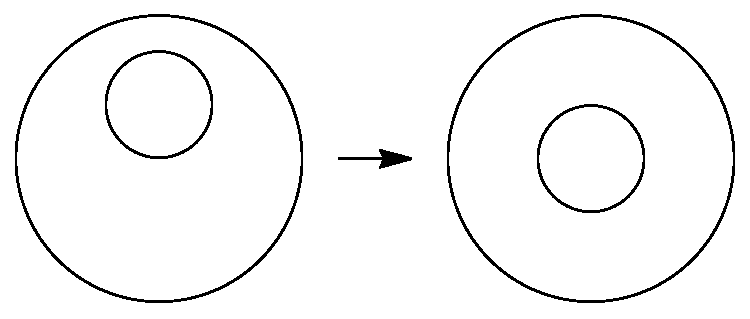
\includegraphics[width=0.7\linewidth]{map.pdf}
	\caption{Non-concentric circles to annulus}
	\label{fig:4}
\end{figure}
Using the fractional part of the transformation from problem 2, we have a map that takes circles at origin and map them to circles centered around some other point. This implies that we can use that map here and we just need to find a value of $\alpha$ which takes the inner circle with origin at $z=c$ and radius $c$ to a circle with origin at $z=0$ and radius $r$. We will assume $\alpha\in \mathds R$, so $\bar \alpha=\alpha$. Mapping the edges of the inner circle to $-r$ and $r$ we find:
\begin{equation}
\begin{aligned}
-r&=f(z=0)=\frac{0-\alpha}{\alpha\times 0-1}=\alpha
\\
r&=f(z=2c)=\frac{2c-\alpha}{2\alpha c-1}\\
\Rightarrow~~~~&2c-\alpha=-\alpha(2\alpha c-1)\\
\Rightarrow~~~~&2\alpha^2c-2\alpha+2c=0\\
\Rightarrow~~~~&\alpha^2c-\alpha+c=0\\
\Rightarrow~~~~&\alpha_\pm =\frac{1\pm\sqrt{1-4c^2}}{2c}\\
\end{aligned}
\end{equation}
The problem states that $0<c<1/2$ and since $|\alpha|<1$ the only valid solution is $\alpha_-$. Inserting this into the map, we find
\begin{equation}
\begin{aligned}
	f(z)&= \frac{z-\frac{1-\sqrt{1-4c^2}}{2c}}{\frac{1-\sqrt{1-4c^2}}{2c} z-1}\\
	&=\frac{1-\sqrt{1-4c^2}-2cz}{2c+(\sqrt{1-4c^2}-1)z},~~~~~~c<1/2
\end{aligned}
\end{equation}
\section*{Problem 4}
\subsection*{Part a}
In this problem we will be using the map from the previous problem. On could do the problem for a general $c$, but we note that (requiring, $c<1/2$) the following values of $c$ simplify the transformation
\begin{lstlisting}
In[238]:= Simplify[
Table[-((-1 + Sqrt[1 - 4 b^2] + 2 b z)/(
2 b + (-1 + Sqrt[1 - 4 b^2]) z)), {b, {1/3, 1/4, 1/5, 2/5}}]]

Out[238]= {-((-3 + Sqrt[5] + 2 z)/(
	2 + (-3 + Sqrt[5]) z)), -((-2 + Sqrt[3] + z)/(
	1 + (-2 + Sqrt[3]) z)), -((-5 + Sqrt[21] + 2 z)/(
	2 + (-5 + Sqrt[21]) z)), (-1 + 2 z)/(-2 + z)}
\end{lstlisting}
The simplest transformation happens at $c=\frac{2}{5}$ meaning the center of the small circle is at $z=\frac{2}{5}$ and the radius is $r=\frac{2}{5}$. In this case we get the simple map
\begin{equation}
	\begin{aligned}
		f(z)
		&=\frac{2z-1}{z-2}
	\end{aligned}
\end{equation}
The potential doesn't change in the region
\begin{equation}
\Delta \phi=0 ~~\text{ in the region }|z| < 1~~\&~~|z-\frac{2}{5}| >\frac{2}{5}
\end{equation}
while it must satisfy the following boundary conditions
\begin{equation}
\begin{aligned}
\phi&=\phi_a~~~~\text{ at } |z|=1\\
\phi&=\phi_b~~~~\text{ at } |z-\frac{5}{2}|=\frac{2}{5}\\
\end{aligned}
\end{equation}
Using the map the boundary conditions on the coaxial cable become
\begin{equation}
	\begin{aligned}
		\Phi&=\phi_a~~~~\text{ at }~~~~ |f|=\frac{1}{2}\\
		\Phi&=\phi_b~~~~\text{ at } ~~~~|f|=1\\
	\end{aligned}
\end{equation}
In the coaxial domain this solves the Laplace equation in cylindrical coordinates which for radial symmetric setups is
\begin{equation}
	\Phi(r)=A_0\log|r|+B_0
\end{equation}
Matching at the boundary 
\begin{equation}
\begin{aligned}
\Phi(1)&=A_0\log|1|+B_0=B_0=\phi_b\\
\Phi(1/2)&=A_0\log|1/2|+\phi_b=\phi_a\Rightarrow A_0=(\phi_a-\phi_b)\log 2
\end{aligned}
\end{equation}
So we get 
\begin{equation}
	\begin{aligned}
	\Phi(f)&=(\phi_a-\phi_b)\log 2\log|f|+\phi_b \\
	\phi(z)&=(\phi_a-\phi_b)\log 2\log|\frac{2z-1}{z-2}|+\phi_b
\end{aligned}
\end{equation}
To write this in terms of $x$ and $y$ coordinates we insert $z=x+iy$ and write the term in the logarithm in terms of its real and complex parts
\begin{equation}
	\begin{aligned}
		\phi(x,y)&=(\phi_a-\phi_b)\log 2\log|\frac{2(x+iy)-1}{(x+iy)z-2}|+\phi_b\\
		&=(\phi_a-\phi_b)\log 2\log|\frac{2 x^2-5 x-2 y^2+2}{x^2-4 x+y^2+4}+i\frac{4 x y-5 y}{x^2-4 x+y^2+4}|+\phi_b
		\\
		&=(\phi_a-\phi_b)\log 2\log\sqrt{\frac{4 x^2-4 x+4 y^2+1}{x^2-4 x+y^2+4}}+\phi_b
		\\
		&=\frac{1}{2}(\phi_a-\phi_b)\log 2\log\frac{4 x^2-4 x+4 y^2+1}{x^2-4 x+y^2+4}+\phi_b
	\end{aligned}
\end{equation}
\subsection*{Part b}
We saw in class (and partially in the last HW), that the (normalized to unity) fluid streamline function for uniform flow can be written as $\Phi(z)=z$. To get the fluid flowing around a corner, which in this case is the lower left quadrant, we want a map which takes values from the quadrant to UHP. One such map is $f(z)=(iz)^{\frac{2}{3}}$, we note however that this is not necesarilly unique, since e.g. the maps $z^{2n}$, $n=1,2,3,\dots$ do the same job.
Using this map for our streamline we simply get
\begin{equation}
\Phi(f)=\Phi((iz)^{\frac{2}{3}})=(iz)^{\frac{2}{3}}
\end{equation}
Or, using the inverse map
\begin{equation}
\phi=-iz^{\frac{3}{2}}
\end{equation}
using this mapping one can write it in terms of real and complex parts as usual
\begin{equation}
\begin{aligned}
x=&-\left(u^2+v^2\right)^{3/4} \cos \left(\frac{3}{2}  \arg[i u - v]\right)\\
y=&\left(u^2+v^2\right)^{3/4}  \sin\left(
\frac{3}{2} \arg[i u - v]
\right)
\end{aligned}
\end{equation}
Finally the streamlines can be sketched holding $u$ constant and varying $v$ using the following code (see next page for the figure)
\begin{lstlisting}
Pot2 = ParametricPlot[{{-(0.5^2 + v^2)^(3/4) Cos[
		3/2 Arg[I 0.5 - v]], (0.5^2 + v^2)^(3/4)
		Sin[3/2 Arg[I 0.5 - v]]}, {-(1^2 + v^2)^(3/4) Cos[
		3/2 Arg[I 1 - v]], (1^2 + v^2)^(3/4)
		Sin[3/2 Arg[I 1 - v]]}, {-(2^2 + v^2)^(3/4) Cos[
		3/2 Arg[I 2 - v]], (2^2 + v^2)^(3/4)
		Sin[3/2 Arg[I 2 - v]]}, {-(3^2 + v^2)^(3/4) Cos[
		3/2 Arg[I 3 - v]], (3^2 + v^2)^(3/4)
		Sin[3/2 Arg[I 3 - v]]}, {-(4^2 + v^2)^(3/4) Cos[
		3/2 Arg[I 4 - v]], (4^2 + v^2)^(3/4) 
		Sin[3/2 Arg[I 4 - v]]},
		{-(5^2 + v^2)^(3/4) Cos[3/2 Arg[I 5 - v]], 
			(5^2 + v^2)^(3/4)
		Sin[3/2 Arg[I 5 - v]]}}, {v, -10, 10}, 
PlotStyle -> {{Red, Thick}, {Red, Thick}}];
Show[Pot2]
\end{lstlisting}
\begin{figure}[H]
	\centering
	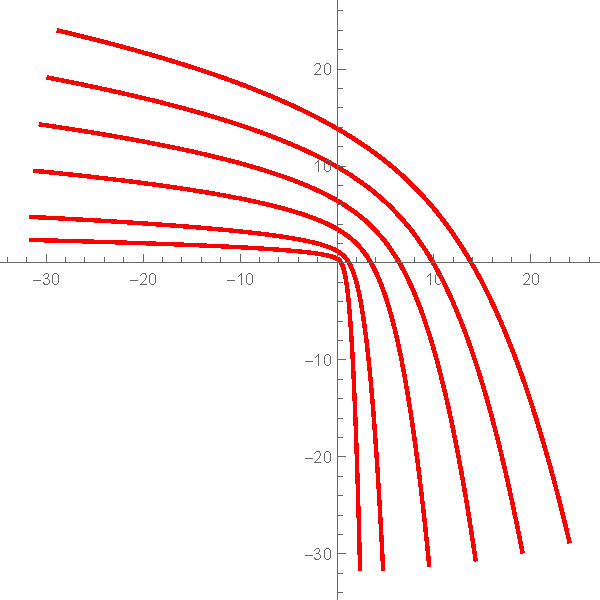
\includegraphics[width=0.6\linewidth]{contour2.pdf}
	\caption{Streamlines around corner}
	\label{fig:4}
\end{figure}
%%%%%%%%%%%%%%%%%%%%%%%%%%%%%%%%%%%%%%%%%%%%%%%%%%%%%%%%%%%%%%%%%%%%
%%%%%%%%%%%%%%%%%%%%%%%%%%%%%%%%%%%%%%%%%%%%%%%%%%%%%%%%%%%%%%%%%%%%
\newpage
\section*{Homework 3\\\\
	Taro V. Brown}\vspace*{1cm}
\section*{Problem 1}
\subsection*{Integral 1}
We want to calulate the integral
\begin{equation}
I_1=\int_{0}^{\infty}\dd x\frac{x^{-a}}{x+1},~~~~~\alpha \in (0,1)
\end{equation}
If we extend this to the complex plane we need to specify a contour which avoids the branch cut along the real axis. A suitable contour is the keyhole (Pac Man) contour, see figure
\begin{figure}[H]
	\centering
	\begin{tikzpicture}
		% Configurable parameters
		\def\gap{0.3}
		\def\bigradius{3}
		\def\littleradius{0.5}
		
		% Axes
		\draw (-1.1*\bigradius, 0) -- (1.1*\bigradius,0) node[right] {$\Re$}
		(0, -1.1*\bigradius) -- (0, 1.1*\bigradius) node[above] {$\Im$};
		% Red path
		\draw[red, thick,   decoration={ markings,
			mark=at position 0.17 with {\arrow{latex}}, 
			mark=at position 0.53 with {\arrow{latex}},
			mark=at position 0.755 with {\arrow{latex}},  
			mark=at position 0.955 with {\arrow{latex}}}, 
		postaction={decorate}]  
		let
		\n1 = {asin(\gap/2/\bigradius)},
		\n2 = {asin(\gap/2/\littleradius)}
		in (\n1:\bigradius) arc (\n1:360-\n1:\bigradius)
		-- (-\n2:\littleradius) arc (-\n2:-360+\n2:\littleradius)
		-- cycle;
		\draw [thick,decorate, decoration=zigzag] (0, 0) -- (3, 0);
		\node at (1.5,0.5) {$C_U$};
		\node at (1.5,-0.5) {$C_L$};
		\node at (-0.5,0.7) {$C_\epsilon$};
		\node at (2,2.7) {$C_R$};
	\end{tikzpicture}
\end{figure}
We then have the contour integral
\begin{equation}
\oint_C\dd z\frac{z^{-a}}{z+1},~~~~~\alpha \in (0,1)
\end{equation}
We start of by noting that the large and small circle contours don't contribute since, by parameterizing and assuming there is no residue at $z=0$\footnote{equivalently we can effectively ignore the $\epsilon$ factor in the denominator} we obtain the integrands integrated from $0$ to $2\pi$
\begin{equation}
\begin{aligned}
	iRe^{i\theta}\dd z\frac{e^{-i\alpha\theta }R^{-a}}{e^{i\theta }R+1}\sim R^{-\alpha}\to 0~~~~\text{ as }~~R\to\infty,~~~~~\text{for }\alpha \in (0,1)\\
	i\epsilon e^{i\theta}\dd z\frac{e^{-i\alpha\theta }\epsilon^{-a}}{e^{i\theta }\epsilon+1}\sim \epsilon^{1-\alpha}\to 0~~~~\text{ as }~~\epsilon\to0,~~~~~\text{for }\alpha \in (0,1)
\end{aligned}
\end{equation}
on the upper contour $z=xe^{0i}$ and on the lower $z=xe^{2\pi i}$, with the only pole inside the contour being the simple pole at $z=-1=e^{i\pi}$. The residue on this pole is easily seen to be $(-1)^{\alpha}=e^{-i\pi \alpha}$ and so the residue theorem then gives (after flipping the integration ranges one of the contours)
\begin{equation}
\begin{aligned}
2\pi i e^{-i\pi \alpha}&=\int_{0}^{\infty}\dd x\,\frac{x^{-\alpha}}{1+x}-\int_{0}^{\infty}\dd x\,\frac{x^{-\alpha}e^{-2\pi i\alpha}}{1+xe^{-2\pi i}}\\
&=\left(1-e^{-2\pi i \alpha}\right)\int_{0}^{\infty}\dd x\,\frac{x^{-\alpha}}{1+x}
\end{aligned}
\end{equation}
which gives us the value of the integral we were looking for, since
\begin{equation}
	\begin{aligned}
		\int_{0}^{\infty}\dd x\,\frac{x^{-\alpha}}{1+x}&=\frac{2\pi ie^{-i\pi \alpha}}{1- ie^{-2i\pi \alpha}}=\frac{\pi}{\sin \pi\alpha}
	\end{aligned}
	\end{equation}
\subsection*{Integral 2}
We now look at the integral
\begin{equation}
I_2=\int_{0}^{\pi}\dd x\,\log(\sin x)
\end{equation}
For this we consider the complex integral 
\begin{equation}
\oint \dd z\,\log(-2ie^{iz}\sin z)
\end{equation}
along the following dented rectangle contour
% TODO: \usepackage{graphicx} required
\begin{figure}[H]
	\centering
	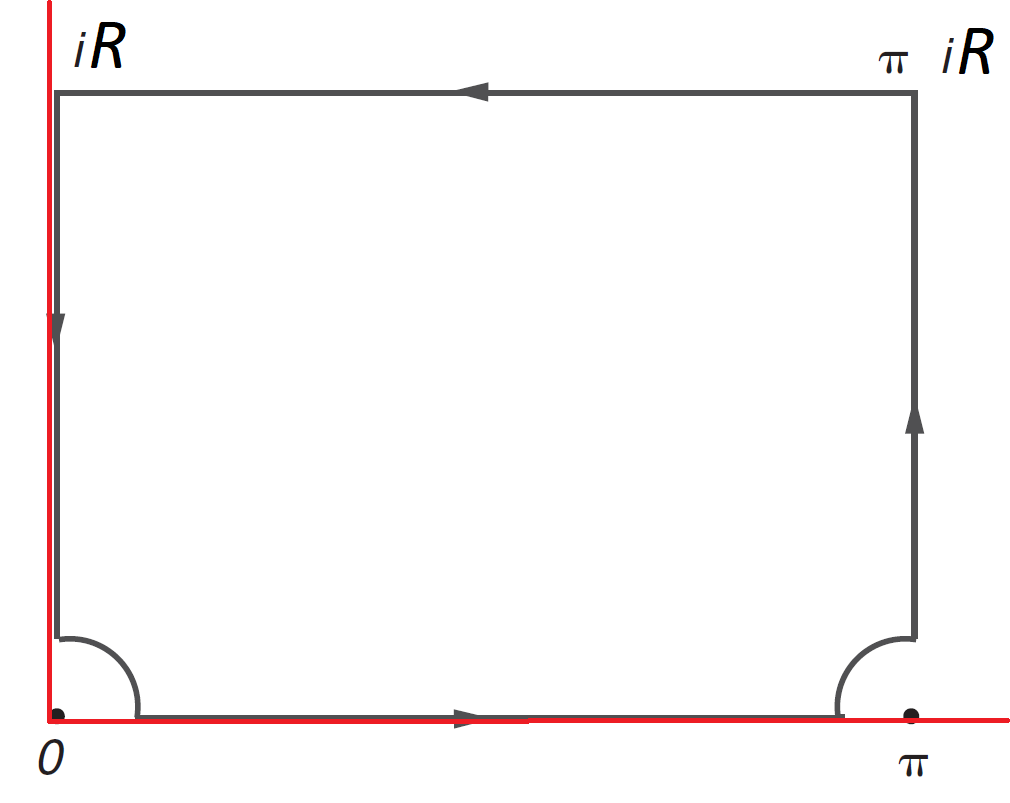
\includegraphics[width=0.5\linewidth]{rectangle}
	\caption{Indented rectangle contour}
	\label{fig:rectangle}
\end{figure}
The integrand is analytic inside this closed contour, and since there are no poles within the contour we get from the residue theorem that the integral along the closed contour vanishes. \\
We start off by looking at the integrand around the indentations. Here we get parameterizations $\epsilon e^{i\theta}$ and $\epsilon e^{i\theta}+\pi$. So the integrands go as
\begin{equation}
\begin{aligned}
&\epsilon \log(-2ie^{i\epsilon e^{i\theta}}\sin {\epsilon e^{i\theta}})\to 0\text{ as } \epsilon \to 0\\
&\epsilon \log(-2ie^{i (\pi +\epsilon e^{i\theta})}\sin {(\pi +\epsilon e^{i\theta})})\to 0\text{ as } \epsilon \to 0
\end{aligned}
\end{equation}
We now find the sum of the integrals of the two vertical contours (parameterizing $z=iR$ in the first and $z=iR+\pi$ on the second)
\begin{equation}
\begin{aligned}
&i\int_{\infty}^{0}\log(-2ie^{-R}\sin iR)+i\int_{0}^{\infty}\log(-2ie^{-R+i\pi}\sin iR+\pi)\\
&=i\int_{\infty}^{0}\log(-2ie^{-R}\sin iR)+i\int_{0}^{\infty}\log(-2ie^{-R}\sin iR)\\
&=
-i\int^{\infty}_{0}\log(-2ie^{-R}\sin iR)+i\int_{0}^{\infty}\log(-2ie^{-R}\sin iR)\\
&=0
\end{aligned}
\end{equation}
For the top of the square we have $z=x+iR$
\begin{equation}
\begin{aligned}
\int_{\pi}^{0}\dd x\log(-2ie^{i(x+iR)}\sin (x+iR))
\end{aligned}
\end{equation}
By letting $R\to\infty$ we get that the integrand goes as
\begin{equation}
	\begin{aligned}
\lim_{R\to\infty}\log(-2ie^{i(x+iR)}\sin (x+iR))&=\frac{1}{2} i k e^{i (x+i R)+R-i x}-\frac{1}{2} i k e^{i (x+i R)-R+i x}\\
&=\lim_{R\to\infty} \log(1+e^{2ix-2R})=0
	\end{aligned}
\end{equation}
Finally we see that only the bottom line segment contributes. Here we get ( setting $z=x$ and expanding the logarithm)
\begin{equation}
	\begin{aligned}
		\int^{\pi}_{0}\dd x\log(-2ie^{ix}\sin (x))&=	\int^{\pi}_{0}\dd x \left(ix+\log 2+\log (\sin x)+\log(-i)\right)\\
		&=	\frac{ix^2}{2}+\pi\log 2+\pi\log(-i)+\int^{\pi}_{0}\dd x \log (\sin x)\\
				&=\pi\log 2+\int^{\pi}_{0}\dd x \log (\sin x)
	\end{aligned}
\end{equation}
Since the closed contour integral was zero along the full contour and all other segments vanished we finally find
\begin{equation}
\int^{\pi}_{0}\dd x \log (\sin x)=-\pi\log 2
\end{equation}
\subsection*{Integral 3}
Lastly we consider the integral
\begin{equation}
I_3=\int_{0}^{\infty}\dd x\,\frac{x^{\alpha-1}}{1+x^4},~~~~~\alpha\in(0,4)
\end{equation}
The complex integrand $f(z)=\frac{z^{\alpha-1}}{1+z^4}$ has poles at $\{e^{3\pi/4},e^{\pi/4},e^{-3\pi/4},e^{-\pi/4}\}$, we will however only consider a contour that encloses $z_0=e^{i\pi/4}$. Let us integrate along a contour in the first quadrant, see figure
\begin{figure}[H]
	\centering
	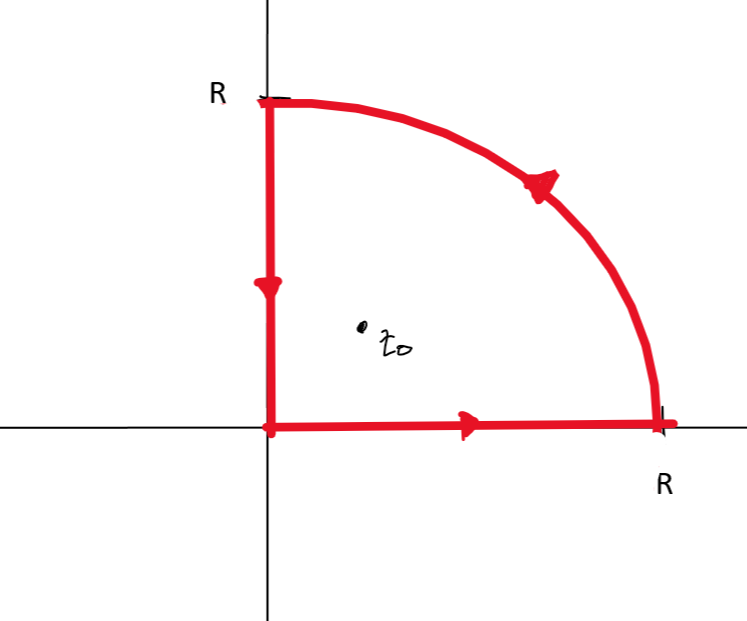
\includegraphics[width=0.5\linewidth]{cont}
	\caption{First quadrant ontour}
	\label{fig:rectangle}
\end{figure}
The complex integral along this contour picks up the following contribution from the residue
\begin{equation}
\oint\dd z\,\frac{z^{\alpha-1}}{1+z^4}=-\frac{i\pi}{2}e^{i\pi\alpha/4} 
\end{equation}
We then consider the individual contributions from the line segments. The quarter circle contributions vanishes as $R\to\infty$, which can be seen by parameterizing $z=Re^{i\theta}$ and looking at the integrand with the Jacobian, explicitly the $R$ goes as
\begin{equation}
\sim R\frac{R^{\alpha-1}}{1+R^{4}}\sim \frac{R^{\alpha}}{R^4}\to 0~~\text{as }~~R\to\infty ~~\text{ for } ~~ \alpha < 4
\end{equation}
The two other segments sum to give the following contribution as we increase the size of the contour (with $z=ix$ for the vertical and $z=x$ for the horizontal segment respectively)
\begin{equation}
\begin{aligned}
\int_\infty^0 i \dd x\,\frac{(ix)^{\alpha-1}}{1+(ix)^4}+\int^\infty_0  \dd x\,\frac{x^{\alpha-1}}{1+x^4}&=(1-i^\alpha)\int^\infty_0  \dd x\,\frac{x^{\alpha-1}}{1+x^4}\\
&=(1-e^{i\pi \alpha/2})\int^\infty_0  \dd x\,\frac{x^{\alpha-1}}{1+x^4}
\end{aligned}
\end{equation}
Setting this equal to the contribution we found from the residue, one obtains
\begin{equation}
\begin{aligned}
\int^\infty_0  \dd x\,\frac{x^{\alpha-1}}{1+x^4}=-\frac{i\pi}{2(1-e^{i\pi \alpha/2})}e^{i\pi\alpha/4}=\frac{\pi}{4\sin \alpha\pi/4}
\end{aligned}
\end{equation}
\section*{Problem 2}
\subsection*{Part a}
We want to show that we can use the following integral
\begin{equation}
\begin{aligned}
I_1=\int_0^\infty \dd z\, f(z)\log z
\end{aligned}
\end{equation}
to compute an integral that isn't symmetric and hence can't be computed emidiatly using Jordan's Lemma, such as the following for $f(x)$ not symmetric:
\begin{equation}
	\begin{aligned}
		I=\int_0^\infty \dd x\, f(x)~~~~~~
	\end{aligned}
\end{equation}
Since our integrand now includes the logarithm we must integrate around a contour that excludes the branch cut, see below:
\begin{figure}[H]
	\centering
  \begin{tikzpicture}
	% Configurable parameters
	\def\gap{0.3}
	\def\bigradius{3}
	\def\littleradius{0.5}
	
	% Axes
	\draw (-1.1*\bigradius, 0) -- (1.1*\bigradius,0) node[right] {$\Re$}
	(0, -1.1*\bigradius) -- (0, 1.1*\bigradius) node[above] {$\Im$};
	% Red path
	\draw[red, thick,   decoration={ markings,
		mark=at position 0.17 with {\arrow{latex}}, 
		mark=at position 0.53 with {\arrow{latex}},
		mark=at position 0.755 with {\arrow{latex}},  
		mark=at position 0.955 with {\arrow{latex}}}, 
	postaction={decorate}]  
	let
	\n1 = {asin(\gap/2/\bigradius)},
	\n2 = {asin(\gap/2/\littleradius)}
	in (\n1:\bigradius) arc (\n1:360-\n1:\bigradius)
	-- (-\n2:\littleradius) arc (-\n2:-360+\n2:\littleradius)
	-- cycle;
	\draw [thick,decorate, decoration=zigzag] (0, 0) -- (3, 0);
	\node at (1.5,0.5) {$C_U$};
	\node at (1.5,-0.5) {$C_L$};
	\node at (-0.5,0.7) {$C_\epsilon$};
	\node at (2,2.7) {$C_R$};
\end{tikzpicture}
\end{figure}
The contour segments are
\begin{equation}
\begin{aligned}
C_R:&~~~~~~~~\text{A circle of radius R}\\
C_\epsilon:&~~~~~~~~\text{A circle of radius }\epsilon\\
C_U:&~~~~~~~~\text{Line segment from $\epsilon+i\epsilon$ to $R+i\epsilon$}\\
C_L:&~~~~~~~~\text{Line segment from from $R-i\epsilon$ to $\epsilon-i\epsilon$}
\end{aligned}
\end{equation}
where we take $\epsilon\to 0$ and $R\to \infty$ at the end. This limit should in most cases make the contributions from the large and small circles go to zero, but this has to be checked on case by case basis. Assuming that this holds we are left with the discontuniuty over the branch cut. If we look at the two line segments we get two integrals that are restricted just above and below the real line 
\begin{equation}
\begin{aligned}
\int_{C_U}\dd z\, f(z)\log z=\int_{\epsilon}^{R} \dd x\, f(x+i \epsilon)\log (x+i\epsilon)\\
\int_{C_L}\dd z\, f(z)\log z=\int_{R}^{\epsilon} \dd x\, f(x-i \epsilon)\log (x-i\epsilon)
\end{aligned}
\end{equation} 
We then use the fact that because of the branch cut
\begin{equation}
\begin{aligned}
\lim_{\epsilon\to 0}\log(x+i\epsilon)&=\log(x)\\
\lim_{\epsilon\to 0}\log(x-i\epsilon)&=\log(x)+2\pi i
\end{aligned}
\end{equation}
Taking the limit we get
\begin{equation}
	\begin{aligned}
		\lim_{\substack{\epsilon\to0\\R\to\infty}}\int_{\epsilon}^{R} \dd x\, f(x+i \epsilon)\log (x+i\epsilon)&=\int^{\infty}_{0} \dd x\, f(x)\log (x)\\
		\lim_{\substack{\epsilon\to0\\R\to\infty}}\int_{R}^{\epsilon} \dd x\, f(x-i \epsilon)\log (x-i\epsilon)&=-\int^{\infty}_{0} \dd x\, f(x)\left(\log (x)+2\pi i\right)\\
	\end{aligned}
\end{equation} 
So that the sum is just
\begin{equation}
\begin{aligned}
\int_{C_U}\dd z\, f(z)\log z+
\int_{C_L}\dd z\, f(z)\log z
&=-2\pi i\int^{\infty}_{0} \dd x\, f(x)\\
&=-2\pi i I
\end{aligned}
\end{equation}
Using this we see that we obtain the integral we wanted, provided that the integrals along the large and small circle contours vanish.
In that case we have
\begin{equation}
I=-\sum_{i}\Res[f(z)\log z]_{z=z_i}
\end{equation}
 We can now use this to calculate the following integrals
\begin{equation}
I_a=\int_0^\infty \dd x \frac{1}{(x+1)(x^2+2x+2)},~~~~I_b=\int_0^\infty\dd x \frac{1}{(x^3+1)}
\end{equation}
Performing the first integral we first check that the contributions from the large and small circles vanish in the appropriate limits by parameterizing $z=Re^{i\theta}$ (large circle) and $z=\epsilon e^{i\theta}$ (small circle). To do this it is convenient to introduce something known as the ML estimate. For an analytic function around some contour $\gamma$ then 
\begin{equation}
\left|\int_\gamma\,\dd z\, f(z)\right|\leq M L
\end{equation}
with L being the length of the contour and M the maximum value of the function on the contour. Taking the large circle contour we parameterize it
\begin{equation}
\begin{aligned}
\int_{C_R} \dd z \frac{\log z}{(x+1)(x^2+2x+2)}&=\int_{0}^{2\pi} i\dd \theta R e^{i\theta} \frac{\log Re^{i\theta}}{(Re^{i\theta}+1)(R^2e^{2i\theta}+2Re^{i\theta}+2)}
\end{aligned}
\end{equation}
The length of the contour is $2\pi R$ and the maximum value is at $2\pi$, so
\begin{equation}
	\begin{aligned}
	 \left|\int_{C_R} \dd z \frac{\log z}{(x+1)(x^2+2x+2)}\right|&\leq(2\pi R)
	 \frac{\log R}{(-R+1)(R^2-2R-2)}\leq2\pi \frac{\log R}{R^2}\to 0 \text{ as } R\to\infty
	\end{aligned}
\end{equation}
For the small circle we will have to assume that the function doesn't blow up around $z=0$. Then the leading order behaviour goes as
\begin{equation}
	\begin{aligned}
		\int_{C_\epsilon} \dd z \frac{\log z}{(x+1)(x^2+2x+2)}&=\int_{\epsilon}^{2\pi-\epsilon} i\dd \theta \epsilon e^{i\theta} \frac{\log \epsilon e^{i\theta}}{(\epsilon e^{i\theta}+1)(\epsilon ^2e^{2i\theta}+2\epsilon e^{i\theta}+2)}\\
			\end{aligned}
	\end{equation}
where the integrand goes as
\begin{equation}
	\begin{aligned}
 \epsilon\log \epsilon \to 0 \text{ as }\epsilon\to 0
	\end{aligned}
\end{equation}
We can now use the residue theorem with the logarithm to find the value of the integral. First factor the integrand
\begin{equation}
\frac{\log z}{(z+1)(z^2+2z+2)}= \frac{\log z}{[z+1]\times \left[z-(i-1)\right]\times \left[z-(-i-1)\right]}
\end{equation}
So we have poles at $\{-1,i-1,-i-1\}$. The exponetial form of these residues are  $\{e^{\pi},\sqrt{2} e^{\frac{3 i \pi }{4}},\sqrt{2} e^{\frac{1}{4} (5 i \pi )}\}$. Taking the residues we then find
\begin{equation}
	\begin{aligned}
	I_a&=-\Res\left[\log z f(z)\right]\Big|_{z=-1}-\Res\left[\log zf(z)\right]\Big|_{z=-1-i}-\Res\left[\log zf(z)\right]\Big|_{z=1-i}\\
	&=-\frac{\log z}{\left[z-(i-1)\right] \left[z-(-i-1)\right]}\Bigg|_{z=-1}-\frac{\log z}{\left[z+1\right] \left[z-(-i-1)\right]}\Bigg|_{z=i-1}-\frac{\log z}{\left[z+1\right] \left[z-(i-1)\right]}\Bigg|_{z=-i-1}\\
	&=-i \pi -\frac{1}{4} \log \left(\frac{1}{2}e^{\frac{5 i \pi }{4}}\right)-\frac{1}{4} \log \left(\frac{1}{2} e^{\frac{3 i \pi }{4}}\right)\\
	&=\frac{\log 2}{2}	\end{aligned}
\end{equation}
For the other integral again use the ML estimate for the large circle contour
\begin{equation}
	\begin{aligned}
		\int_{C_R} \dd z \frac{\log z}{(z^3+1)}&=\int_{0}^{2\pi} i\dd \theta R e^{i\theta} \frac{\log Re^{i\theta}}{(R^3e^{3i\theta}+1)}
	\end{aligned}
\end{equation}
So
\begin{equation}
	\begin{aligned}
		\left|\int_{C_R} \dd z \frac{\log z}{(z^3+1)}\right|&\leq(2\pi R)
		\frac{\log R}{(R^3+1)}\leq2\pi \frac{\log R}{R^2}\to 0 \text{ as } R\to\infty
	\end{aligned}
\end{equation}
While, for the small circle
\begin{equation}
	\begin{aligned}
		\int_{C_\epsilon} \dd z \frac{\log z}{(x+1)(x^2+2x+2)}&=\int_{\epsilon}^{2\pi-\epsilon} i\dd \theta \epsilon e^{i\theta} \frac{\log \epsilon e^{i\theta}}{(\epsilon e^{i\theta}+1)(\epsilon ^2e^{2i\theta}+2\epsilon e^{i\theta}+2)}\\
	\end{aligned}
\end{equation}
where the integrand again goes as
\begin{equation}
	\begin{aligned}
		\epsilon\log \epsilon \to 0 \text{ as }\epsilon\to 0
	\end{aligned}
\end{equation}
Hence contributions from both circles vanish. We then factor the integrand like before
\begin{equation}
\begin{aligned}
	\frac{\log z}{(z^3+1)}&= \frac{\log z}{[z-(-1)]\times \left[z-(-1)^{1/3}\right]\times \left[z-(-(-1)^{2/3})\right]}\\
	 &=\frac{\log z}{[z+1)]\times \left[z-(-1)^{1/3}\right]\times \left[z+(-1)^{2/3}\right]}
\end{aligned}
\end{equation}
The residues can also be written as $\{z=e^{i\pi},z=e^{\frac{i \pi }{3}},z=e^{\frac{5 i \pi }{3}}\}$
And evalue the residues at these poles
\begin{equation}\hspace*{-1cm}
	\begin{aligned}
		I_a&=-\Res\left[\log z f(z)\right]\Big|_{z=-1}-\Res\left[\log zf(z)\right]\Big|_{z=(-1)^{1/3}}-\Res\left[\log zf(z)\right]\Big|_{z=-(-1)^{2/3}}\\
		&=-\frac{\log z}{\left[z-(-1)^{1/3}\right] \left[z+(-1)^{2/3}\right]}\Bigg|_{z=-1}-\frac{\log z}{[z+1] \left[z+(-1)^{2/3}\right]}\Bigg|_{z=(-1)^{1/3}}-\frac{\log z}{[z+1] \left[z-(-1)^{1/3}\right]}\Bigg|_{z=-(-1)^{2/3}}\\
		&=-i\pi/3+5/9(-1)^{1/6}+1/9(-1)^{5/6}\pi\\
		&=\frac{2 \pi }{3 \sqrt{3}}
	\end{aligned}
\end{equation}
\subsection*{Problem 3}
\subsection*{Part a}
We want to prove the Mittag-Leffler decomposition
\begin{equation}
f(z)=f(0)+\sum_{j=1}^{\infty }r_j\left(\frac{1}{z-z_j}+\frac{1}{z_j}\right)
\end{equation}
First we assume that all the poles of $f(z)$ are simple as well as considering a contour enclosing $n$ poles for which $|z_1|<|z_2|<\dots$. Then by the residue theorem we can split this into the poles of $f(w)$ and the pole at $w=z$.
\begin{equation}
\begin{aligned}
\frac{1}{2\pi i}\oint_\gamma \frac{f(w)}{w-z}dw&=\Res(\frac{f(w)}{w-z})\Big|_{w=z}+\sum_j\Res(\frac{f(w)}{w-z})\Big|_{w=z_j}\\
&=\lim_{w\to z}\left(\frac{(w-z)f(w)}{w-z}\right)+\sum_j\lim_{w\to n}\left(\frac{(w-z_j)f(w)}{w-z}\right)\\
&=f(z)+\sum_j\lim_{w\to z_j}\left[\frac{(w-z_j)f(w)}{w-z}\right]\\
\end{aligned}
\end{equation}
The limit on the rhs can be written as a product of the residues of $f$ at $n$ divided by $z_j-z$. Denoting the residues by $r_j$, we then have
\begin{equation}
\begin{aligned}
\frac{1}{2\pi i}\oint_\gamma \frac{f(w)}{w-z}dw&=f(z)+\sum_j\frac{r_j}{z_j-z}\\
\end{aligned}
\end{equation}
Setting $z=0$ we get
\begin{equation}
	\begin{aligned}
		\frac{1}{2\pi i}\oint_\gamma \frac{f(w)}{w}dw&=f(0)+\sum_j\frac{r_j}{z_j}\\
	\end{aligned}
\end{equation}
So we get
\begin{equation}
\frac{1}{2\pi i}\oint_\gamma f(w)\left(\frac{1}{w-z}-\frac{1}{w}\dd w\right)=f(z)-f(0)+\sum_{j=0}^{\infty }r_j\left(\frac{1}{z-z_j}+\frac{1}{z_j}\right)
\end{equation}
If we now assume $f(z)$ to be bounded within the contour for all poles then the contour integral in the above expression vanishes and we get the expression requested
\begin{equation}
f(z)=f(0)+\sum_{j=0}^{\infty }r_j\left(\frac{1}{z-z_j}+\frac{1}{z_j}\right)
\end{equation}
\subsection*{Part b}
If we assume the function $g(z)$ only has simple poles at positions $z_i$, then the function
\begin{equation}
f(z)=\dv{\log(g(z))}{z}=\frac{g'(z)}{g(z)}
\end{equation}
is meromorphic with the same poles. Residues of these poles can be found using L'Hôpitals rule
\begin{equation}
	\begin{aligned}
\Res(f(z))\big|_{z=z_i}&=\lim_{z\to z_i}(z-z_i)f(z)\\
&=\lim_{z\to z_i}\frac{zg'(z)-z_ig'(z)}{g(z)}\\
&=\lim_{z\to z_i}\frac{g'(z)+zg''(z)-z_ig''(z)}{g'(z)}\\
&=\frac{g'(z_i)}{g'(z_i)}\\
&=1~~~\forall \,i \text{ inside $\gamma$ }
	\end{aligned}
\end{equation}

So 
\begin{equation}
\dv{\log(g(z))}{z}=\frac{g'(z)}{g(z)}\Big|_{z=0}+\sum_{j=1}^{\infty }\left(\frac{1}{z-z_j}+\frac{1}{z_j}\right)
\end{equation}
Integrating up on both sides
\begin{equation}
\int_0^z \dd\log(g(z))=\int_0^z \dd z\frac{g'(z)}{g(z)}\Big|_{z=0}+\sum_{j=1}^{\infty }\left(\frac{z}{z_j}+\log(1-\frac{z}{z_j})\right)
\end{equation}
and defining $c\equiv \frac{g'(z)}{g(z)}\Big|_{z=0}$, we get
\begin{equation}
\log g(z)-\log g(0)=cz+\sum_{j=1}^{\infty }\left(\frac{z}{z_j}+\log(1-\frac{z}{z_j})\right)
\end{equation}
which after exponentiation leads to
\begin{equation}
g(z)=e^{cz}g(0)\prod_{j=1}^{N}\left(1-\frac{z}{z_j}\right)e^{z/z_j}
\end{equation}
\section*{Problem 4}
\subsection*{Part a}
We consider the function
\begin{equation}
\cot z=\frac{1}{\tan z}
\end{equation}
This has zeroes at $\pi n$ with $n\in \mathds {Z}$. The residues evaluate to $1$ since from L'Hôpitals rule
\begin{equation}
\begin{aligned}
\Res\left[\cot z\right]\Big|_{z=\pi n}&=\lim_{z\to\pi n}(z-\pi n)\cot( z)\\
&=\lim_{z\to\pi n}(z-\pi n)\frac{\cos z}{\sin z}\\
&=\lim_{z\to\pi n}\frac{\cos z-(z-\pi n)\sin z}{\cos z}\\
&=1
\end{aligned}
\end{equation}
Inserting this into the ML expansion, we first subtract the pole at $z=0$
\begin{equation}
\begin{aligned}
\cot z-\frac{1}{z}=\sum_{j=\infty}^{~~\infty ~~,}\left(\frac{1}{z-\pi n}+\frac{1}{\pi n}\right)
\end{aligned}
\end{equation}
The negative and postive parts of the sum converge independently and so we can split the sum as follows
\begin{equation}
	\begin{aligned}
		\cot z-\frac{1}{z}
				&=\sum_{j=1}^{\infty}\left(\frac{1}{z-\pi n}+\frac{1}{\pi n}+\frac{1}{z+\pi n}-\frac{1}{\pi n}\right)\\
		&=\sum_{j=1}^{\infty}\left(\frac{1}{z-\pi n}+\frac{1}{z+\pi n}\right)\\
		&=\sum_{j=1}^{\infty}\left(\frac{2z}{z^2-\pi^2 n^2}\right)
	\end{aligned}
\end{equation}
From this we get the requested equation
\begin{equation} 
	\cot(z)=\frac{1}{z}+\sum_{n=1}^{\infty}\frac{2z}{z^2-\pi^2 n^2}
\end{equation}
Which can also be written in the convention form
\begin{equation} \label{eq:expansion}
	\cot(z\pi)\pi=\frac{1}{z}+\sum_{n=1}^{\infty}\frac{2z}{z^2-n^2}
\end{equation}
%%%%%%%%%%%%%%%%%%%%%%%%%%%%%%%%%%%%%%%%%%%%%%%%%%%%%%%%%
To show the Lipshitz formula we first write the lhs in terms of exponential functions and use the binomial expansion assuming $\Im z>0$
\begin{equation}
	\cot(z\pi)\pi=-\pi i\frac{e^{2\pi iz}+1}{1-e^{2\pi iz}}=-\pi i\left(e^{2\pi iz}+1\right)\sum_{n=0}^{\infty}e^{2n\pi iz}=-2\pi i\left(\frac{1}{2}+\sum_{n=1}^{\infty}e^{2n\pi iz}\right)
\end{equation}
Taking the derivative of this $k\geq 1$ times we obtain
\begin{equation} \label{eq:dcot}
	\dv[k]{\cot(z\pi)\pi}{z}=(-2\pi i)(2\pi i)^{k}\sum_{n=1}^{\infty}n^k e^{2n\pi iz}
\end{equation}
The rhs of \eqref{eq:expansion} can be rewritten by expanding and grouping the sum
\begin{equation}
\frac{1}{z}+\sum_{n=1}^{\infty}\frac{2z}{z^2-n^2}=\frac{1}{z}+\sum_{n=1}^{\infty}\,\left(\frac{1}{z+n}+\frac{1}{z-n}\right)=\lim_{N\to\infty}\sum_{n=-N}^{N}\frac{1}{z+n}
\end{equation}
Now taking the derivative of this $k\geq 1$ times we, while taking the $N\to \infty $ limit, get
\begin{equation}
\sum_{n=-\infty}^{\infty}\frac{1}{(z+n)^k}(-1)^k k!
\end{equation}
Hence combinging this with \eqref{eq:dcot} we get the requested form
\begin{equation}
\sum_{n=-\infty}^{\infty}\frac{1}{(z+n)^k}=\frac{(-2\pi i)^{k+1}}{k!}\sum_{n=1}^{\infty}n^k e^{2\pi iz}
\end{equation}
\subsection*{Part b}
If we let $g(z)=\frac{\sin z}{z}$ then $g(0)=1$ and $c=0$. The residues are all of unit value at $z=2n\pi$ and the function is entire, so we can use the product expansion from problem 3 to find
\begin{equation}
\frac{\sin z}{z}=\prod_{n=1}^{\infty}\left(1-\frac{z}{n\pi}\right)\left(1+\frac{z}{n\pi}\right)e^{\frac{z}{n\pi}}e^{-\frac{z}{n\pi}}=\prod_{n=1}^{\infty}\left(1-\frac{z^2}{n^2\pi^2}\right)
\end{equation}
Which means that $\sin z$ does have an infinite product expansion. We will now derive the same result from the expression of $\cot z$ we showed in the previous problem. First noting that
\begin{equation}
\cot -\frac{1}{z}=\dv{\log(\frac{\sin z}{z})}{z}
\end{equation}
So using the expantion we found in the previous problem
\begin{equation}
\begin{aligned}
\dv{\log(\frac{\sin z}{z})}{z}&=\sum_{n=1}^{\infty}\frac{2z}{z^2-\pi^2 n^2}\\
&=\dv{\sum_{n}\log(z^2-n^2\pi^2)}{z}
\end{aligned}
\end{equation}
which we can integrate up to get
\begin{equation}
\log(\frac{\sin z}{z})=\sum_{n}\log(z^2-n^2\pi^2)
\end{equation}
or
\begin{equation}
\frac{\sin z}{z}=-\frac{1}{n^2\pi^2}\prod_{n=1}^{\infty}(z^2-n^2\pi^2)=\prod_{n=1}^{\infty}\left(1-\frac{z^2}{n^2\pi^2}\right)
\end{equation}
As per the problem statement. For the case of the Gamma function we know from the recurrence relation
\begin{equation}
\Gamma(z)=\frac{\Gamma(z+n)}{z(z+1)\cdots (z+n-1)}
\end{equation}
that it has poles at $\{0,-1,-2,-3,\cdots\}$ with residues at the $z=-n$ pole being $\frac{num(-1)^n}{n!}$. This was shown in lecture. From this we can deduce that the function $\frac{1}{z\Gamma(z)}$ has zeros at $z=\{-1,-2,-3\cdots\}$. 

Lastly, since the following integral representation converges for all $z$ on the contour $C$ that originates at $-\infty$ just below the real axis and ends at $-\infty$ just above the real axis, after having gone around the origin in a small circle, thereby avoiding the branchcut
\begin{equation}
\frac{1}{\Gamma(z)}=\frac{1}{2\pi i}\int_C\dd t\, \frac{e^t}{t^2}
\end{equation}
the function is entire and we are able to use the expansion from problem 3. USing the product expansion we first have
\begin{equation}
\begin{aligned}
\frac{1}{\Gamma(z+1)}=\frac{1}{z\Gamma(z)}=\Gamma(0+1)e^{cz}\prod_{n=1}^{\infty}\left(1+\frac{z}{n}\right)e^{-\frac{z}{n}}
\end{aligned}
\end{equation}
Using $\Gamma(1)=1$ and $\Gamma'(z)=-\gamma$, with $\gamma $ being the Euler-Mascheroni constant, we find
\begin{equation}
	\begin{aligned}
\frac{1}{\Gamma(z)}=ze^{\gamma z}\prod_{n=1}^{\infty}\left(1+\frac{z}{n}\right)e^{-\frac{z}{n}}
	\end{aligned}
\end{equation}
We can then find the formula requested
\begin{equation}
\begin{aligned}
\frac{1}{\Gamma(z)\Gamma(1-z)}&=
\frac{1}{-z\Gamma(z)\Gamma(-z)}\\
&=z\prod_{n=1}^{\infty}\left(1+\frac{z}{n}\right)\left(1-\frac{z}{n}\right)e^{-\frac{z}{n}}e^{\frac{z}{n}}\\
&=z\prod_{n=1}^{\infty}\left(1-\frac{z^2}{n^2}\right)\\
&=\frac{\sin \pi z}{\pi}
\end{aligned}
\end{equation}
where we have used the just derived result for $\sin z$. Hence we get the equation
\begin{equation}
\Gamma(z)\Gamma(1-z)=\pi\text{cosec} \pi z
\end{equation}
\section{d}
\newpage
%%%%%%%%%%%%%%%%%%%%%%%%%%%%%%%%%%%%%%%%%%%%%%%%%%%%%%%%%%%%%%%%%%%%
%%%%%%%%%%%%%%%%%%%%%%%%%%%%%%%%%%%%%%%%%%%%%%%%%%%%%%%%%%%%%%%%%%%%
\section*{Homework 4\\\\
	Taro V. Brown}\vspace*{1cm}
\section*{Problem 1}
Want to solve ODE
\begin{equation}
	\begin{aligned}
		L_{zz}\phi(z)=\left[\dv[2]{}{z}+\frac{1}{z}\dv{}{z}+\left(1-\frac{\nu^2}{z^2}\right)\right]\phi(z)=0
	\end{aligned}
\end{equation}
Given the kernel
\begin{equation}
	\begin{aligned}
		K(z,t)=\left(\frac{z}{2}\right)^\nu\exp[z-\frac{z^2}{4t}]
	\end{aligned}
\end{equation}
such that
\begin{equation}
\phi(z)=\int_{C} K(z,t)\xi(t)\, \dd t
\end{equation}
Applying the different parts of $L_{zz}$
\begin{equation}
	\begin{aligned}
		\dv[2]{}{z}K=&2^{-\nu } (\nu -1) \nu  e^{z-\frac{z^2}{4 t}} z^{\nu -2}+2^{1-\nu } \nu  e^{z-\frac{z^2}{4 t}} \left(1-\frac{z}{2 t}\right) z^{\nu -1}\\
		&+2^{-\nu } e^{z-\frac{z^2}{4 t}} \left(1-\frac{z}{2 t}\right)^2 z^{\nu }-\frac{2^{-\nu -1} e^{z-\frac{z^2}{4 t}} z^{\nu }}{t}\\
		=&\frac{2^{-\nu -2} e^{z-\frac{z^2}{4 t}} z^{\nu -2} \left(4 t^2 \left((\nu +z)^2-\nu \right)-2 t z^2 (2 \nu +2 z+1)+z^4\right)}{t^2}
	\end{aligned}
\end{equation}
Similarly
\begin{equation}
	\begin{aligned}
		\frac{1}{z}\dv[]{}{z}K=&\frac{2^{-\nu } \nu  e^{z-\frac{z^2}{4 t}} z^{\nu -1}+2^{-\nu } e^{z-\frac{z^2}{4 t}} \left(1-\frac{z}{2 t}\right) z^{\nu }}{z}\\
		=&-\frac{2^{-\nu -1} e^{z-\frac{z^2}{4 t}} z^{\nu -2} \left(z^2-2 t (\nu +z)\right)}{t}
	\end{aligned}
\end{equation}
and finally 
\begin{equation}
	\begin{aligned}
		\left(1-\frac{\nu^2}{z^2}\right)K=&2^{-\nu } e^{z-\frac{z^2}{4 t}} z^{\nu } \left(1-\frac{\nu ^2}{z^2}\right)
	\end{aligned}
\end{equation}
Putting it all together we get 
\begin{equation}
	\begin{aligned}
		\oint_C  \left[\frac{2^{-\nu -2} e^{t-\frac{z^2}{4 t}} z^{\nu +2}}{t^2}+2^{-\nu } e^{t-\frac{z^2}{4 t}} z^{\nu }-\frac{2^{-\nu } e^{t-\frac{z^2}{4 t}} z^{\nu }}{t}-\frac{2^{-\nu } \nu  e^{t-\frac{z^2}{4 t}} z^{\nu }}{t}\right]\xi(t)\,\dd t
	\end{aligned}
\end{equation}
which is the same as 
\begin{equation}
	\begin{aligned}
			\int_C  \xi(t)\left[\dv{}{t}-\frac{\nu+1}{t}\right]K(x,t)\,\dd t	
	\end{aligned}
\end{equation}
Using integration by part to expand this, $L_{zz}\phi(z)=0$ is satisfied by finding a $\xi(t)$ for which 
\begin{equation}
	\begin{aligned}
		-\left[\dv{}{t}+\frac{\nu+1}{t}\right]\xi(t)=0
	\end{aligned}
\end{equation} 
Which leads to $\xi(t)=t^{-\nu-1}$, hence
\begin{equation}
	\begin{aligned}
		J(z)=\frac{1}{2\pi i}\int_C\dd t\, t^{-\nu-1}\left(\frac{z}{2}\right)^\nu\exp[t-\frac{z^2}{4t}]
	\end{aligned}
\end{equation}
Further, the boundary terms have to vanish 
\begin{equation}
	\begin{aligned}
		\left[t^{-\nu-1}\left(\frac{z}{2}\right)^\nu\exp[t-\frac{z^2}{4t}]\right]_{\partial C}=0
	\end{aligned}
\end{equation}
This holds for  $t=-\infty \pm i\epsilon$ and hence we can use the Hankel contour along the negative real axis, see figure below.
\begin{figure}[H]
	\centering
	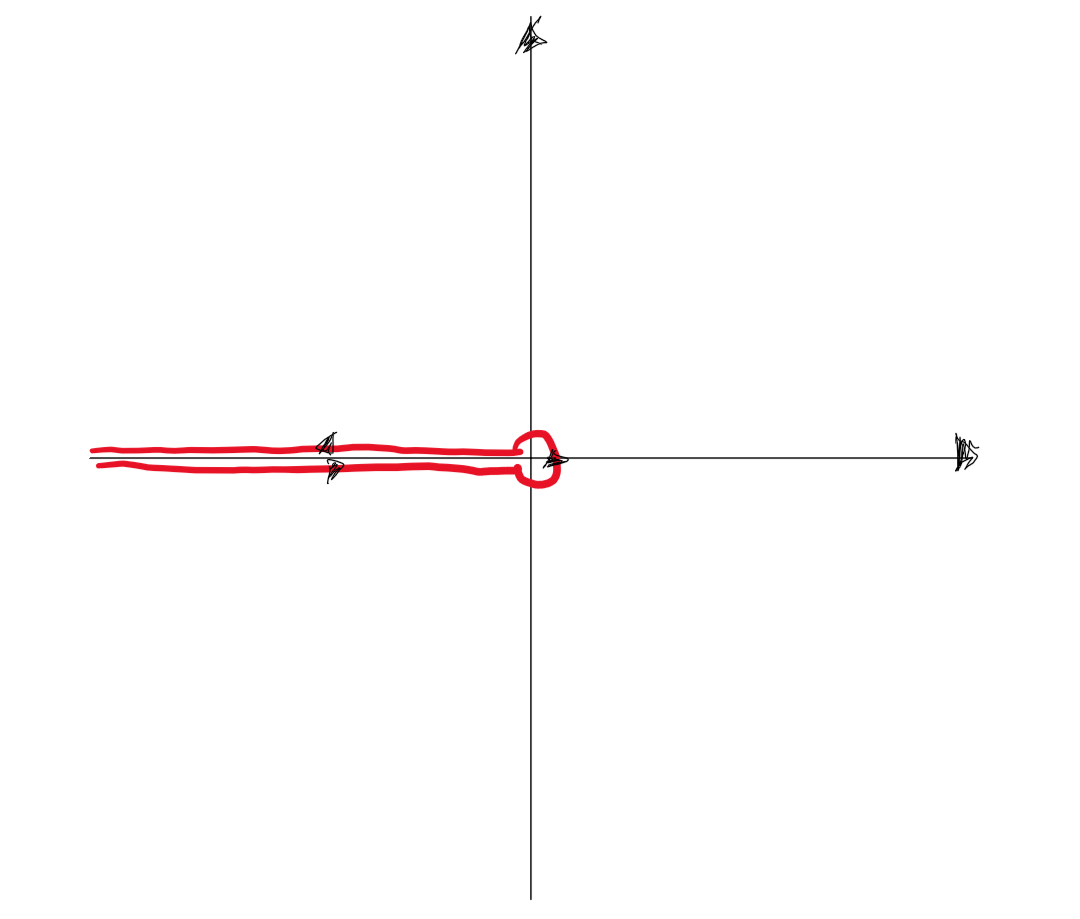
\includegraphics[width=0.45\linewidth]{27}
	\caption{Hankel contour}
	\label{fig:rectangle}
\end{figure}
No information on $\nu$ has been given, so assuming it is not an integer, we need a branch cut integral. Setting first $t=uz/2$ and then $t=e^w$ we get a new contour integral,
\begin{equation}
	\begin{aligned}
		J_\nu(z)=\frac{1}{2\pi i} \int_\gamma \dd w\, e^{z\sinh{w} -vw}
	\end{aligned}
\end{equation}
over the contour shown in the figure below
\begin{figure}[H]
	\centering
	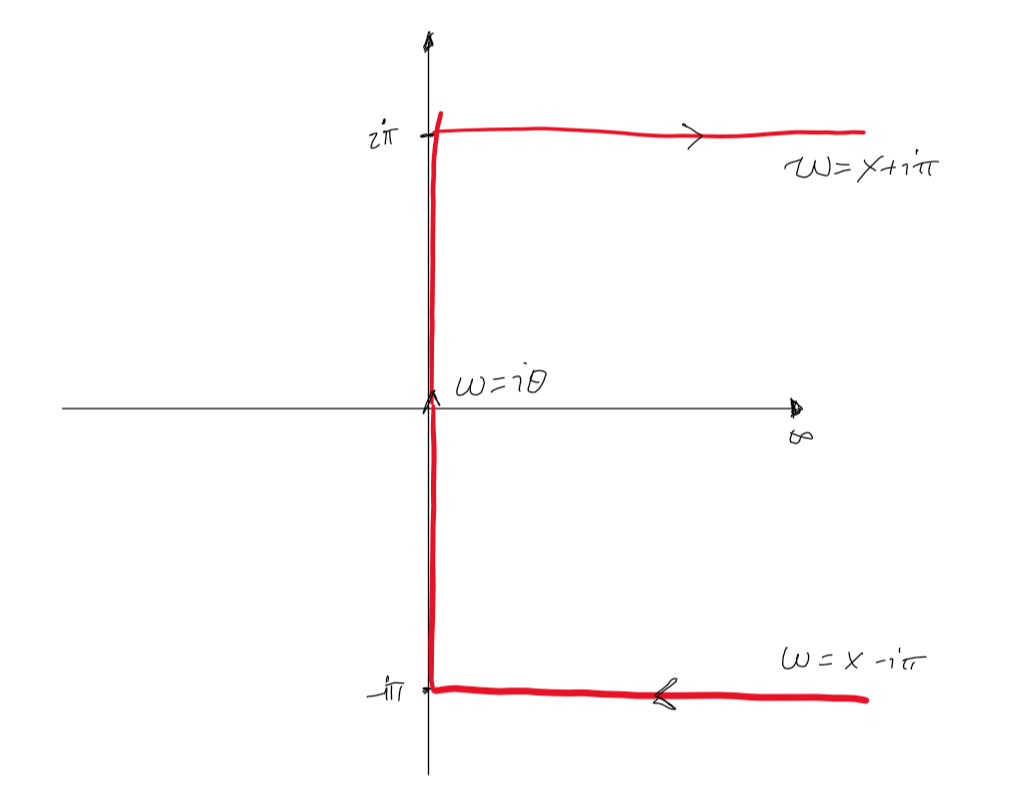
\includegraphics[width=0.5\linewidth]{26}
	\caption{Deformed contour for $J_\nu(z)$}
	\label{fig:rectangle}
\end{figure}
Splitting the contour integral into 2 pieces and setting $w=t+i\pi$ on the flat and $w=i\theta$ on the vertical parts, we get
\begin{equation}
	\begin{aligned}
	J_\nu(z)=\frac{1}{\pi} \int_0^\pi \dd \theta\cos(\nu\theta -z\sin\theta)
	-\frac{\sin\nu\pi}{\pi} \int_0^\infty\dd t e^{-vt-z\sinh t}
	\end{aligned}
\end{equation}
To make sure we have independent solutions of $J_{\nu}$ from $J_{-\nu}$ we then define the Neumann function
\begin{equation}
	\begin{aligned}
		N_\nu(z)\equiv& \frac{J_\nu(z)\cos{\nu\pi-J_{-\nu}(z)}}{\sin{\nu\pi}}\\
		=&
		\int_0^\pi \frac{\cot{\nu\pi}}{\pi}\cos(\nu\theta -z\sin\theta)-\frac{\pi}{\sin{\nu\pi}}\cos(\nu\theta +z\sin\theta)\dd \theta\\
		&- \int_0^\infty \frac{\cos\nu\pi}{\pi} e^{-vt-z\sinh t}+\frac{1}{\pi} e^{vt-z\sinh t}\dd t
	\end{aligned}
\end{equation}
We now define the simpler Hankel functions 
\begin{equation}
	\begin{aligned}
		H_\nu^{(1)}(z)&=\frac{1}{i\pi }\int_{-\infty}^{\infty+i\pi}e^{z\sinh w-vw}\dd w,~~~~~~|\arg z|<\pi/2\\
	H_\nu^{(2)}(z)&=-\frac{1}{i\pi }\int_{-\infty}^{\infty-i\pi}e^{z\sinh w-vw}\dd w,~~~~~~|\arg z|<\pi/2\\
	\end{aligned}
\end{equation}
Their contour integrals go like
\begin{figure}[H]
	\centering
	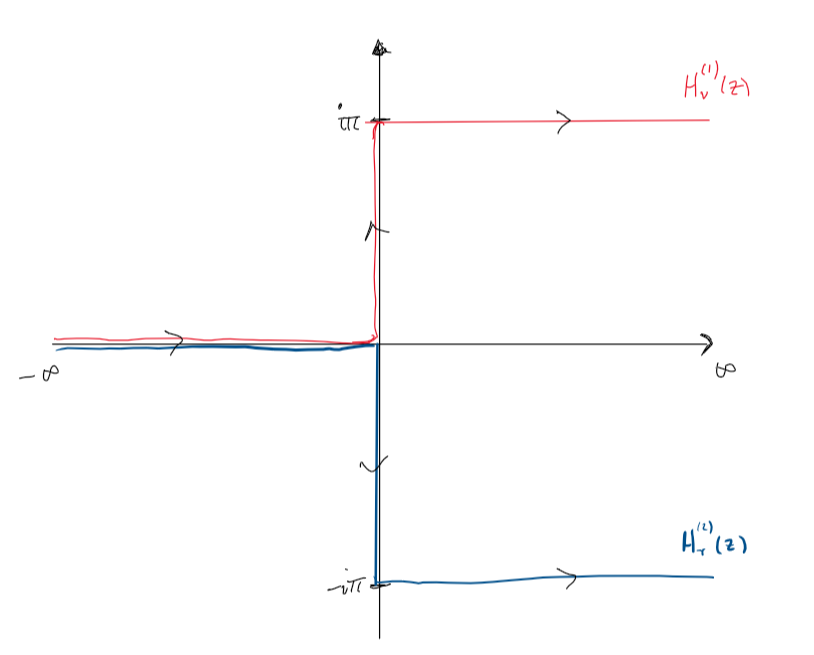
\includegraphics[width=0.55\linewidth]{25}
	\caption{$H_{\nu}^{(1)}(z)$ and $H_{\nu}^{(2)}(z)$ contours.}
	\label{fig:rectangle}
\end{figure}
Let us see what happens when they are combined. We write the sum and split the contour into a part from $\infty$ to 0 (this is canceled by the sum), then a part from $0$ to $\pi$ with $w=i\theta$ and then lastly a part from 0 to $\infty$ with $w=x\pm i\pi$ (depending on the which one of the Hankel functions).

Doing this one obtains the following
\begin{equation}
	\begin{aligned}
		H_\nu^{(1)}(z)+H_\nu^{(2)}(z)\\
		=&\frac{1}{i\pi}\int_{0}^{\infty}e^{z\sinh (x+i\pi)-v(x+i\pi)}\dd 
	x-\frac{1}{i\pi}\int_{0}^{\infty}e^{z\sinh (x-i\pi)-v(x-i\pi)}\dd x\\
&-\frac{1}{i\pi}\int_{0}^{\pi}e^{z\sinh i\theta -\nu i\theta)}i\dd \theta\\
	 =&\frac{1}{\pi}\int_0^\pi e^{i(\nu\theta-z\sinh\theta)}+e^{-i(\nu\theta-z\sinh\theta)}\dd \theta\\
	 &-\frac{1}{\pi}\int_0^\infty \left(e^{i\nu\pi}-e^{-i\nu\pi}\right)e^{-\nu x-z\sinh\theta x}\dd  x
	\end{aligned}
\end{equation}
Converting the exponentials we see that we match the Bessel function just found
\begin{equation}
	\begin{aligned}
		H_\nu^{(1)}(z)+H_\nu^{(2)}(z)=&\frac{2}{\pi} \int_0^\pi \dd \theta\cos(\nu\theta -z\sin\theta)
		-\frac{2\sin\nu\pi}{\pi} \int_0^\infty\dd t e^{-vt-z\sinh t}\\
		&=
		2J_\nu(z)
	\end{aligned}
\end{equation}
Similarly we take take the difference between the two Hankel functions and obtain in the end an expression for $N_\nu(z)$.
\begin{equation}
	\begin{aligned}
		H_\nu^{(1)}(z)-H_\nu^{(2)}(z)\\
		=&\frac{2}{i\pi}\int_{-\infty}^{0}e^{z\sinh x-\nu x}\dd 
		x+\frac{1}{i\pi}\int_{0}^{\infty}e^{z\sinh (x-i\pi)-\nu(x-i\pi)}\dd x\\
		&+\frac{1}{i\pi}\int_{0}^{\infty}e^{z\sinh (x+i\pi)-\nu(x+i\pi)}\dd x+\frac{1}{i\pi}\int_{0}^{\pi}e^{z\sinh i\theta -\nu i\theta}i\dd \theta\\
		&+\frac{1}{i\pi}\int_{0}^{-\pi}e^{z\sinh i\theta -\nu i\theta}i\dd \theta
		\\ 
		=&-\frac{2}{\pi}\int_{0}^{\infty}\left(e^{\nu x}+\cos{\nu x}e^{-\nu x}\right)e^{-\sinh x}\dd x+\frac{1}{\pi}\int_{0}^{\pi}\sin(z\sin\theta-\nu\theta)\dd \theta
		\\
		=& 2N_\nu(z)
	\end{aligned}
\end{equation}
where the last line comes from a definition of $N_\nu(z)$ which can be looked up in an integral table, for instance the one provided in the homework statement.

Finally we want to obtain an expression for the asymptotic expansion of $J_\nu(z)$ and $N_\nu(z)$ using the above representations, using the methods of steepest descent. We will look at the Hankel functions and shift to the Hankel contour for the computation of $J_\nu(z)$ and $N_\nu(z)$, which means the Hankel functions are integrated over the following contours
\begin{equation}
	\begin{aligned}
		H_\nu^{(1)}(z)&=\frac{1}{i\pi }\int_{i\epsilon}^{-\infty+i\epsilon}\dd t\, t^{-\nu-1}e^{-\frac{1}{2}(t-\frac{1}{t})z}\\
		H_\nu^{(2)}(z)&=\frac{1}{i\pi }\int^{-i\epsilon}_{-\infty-i\epsilon}\dd t\, t^{-\nu-1}e^{-\frac{1}{2}(t-\frac{1}{t})z}
	\end{aligned}
\end{equation}
The saddlepoint is easily found
\begin{equation}
	\begin{aligned}
		\dv{}{t}(1-1/t)\big|_{t=t_0}=0\Rightarrow t_0=\pm i
	\end{aligned}
\end{equation}
For $H_\nu^{(1)}(z)$ and $H_\nu^{(2)}(z)$ we have to derform the contour in different ways to go through the saddle point. Picking $i$ for $H_\nu^{(1)}(z)$ and $-i$ for $H_\nu^{(2)}(z)$. We start of by doing $H_\nu^{(1)}(z)$ and translate the result to $H_\nu^{(2}(z)$. 

First we define $\xi\equiv t-i$, then we expand around the saddle point, assuming that $z$ is large
\begin{equation}
	\begin{aligned}
		H_\nu^{(1)}(z)&=\frac{1}{i\pi }\int_{i\epsilon}^{-\infty+i\epsilon}\dd \xi\, (\xi+i)^{-\nu-1}e^{-\frac{1}{2}(\xi+i-\frac{1}{\xi+i})z}\\
		&=\frac{1}{i\pi }\int_{i\epsilon}^{-\infty+i\epsilon}\dd \xi\, (\xi+i)^{-\nu-1}e^{iz-i\frac{z}{2}\xi^2+\mathcal{O}(\xi^3)}\\
	\end{aligned}
\end{equation}
We then take $\xi=r e^{i\theta}$ and expand the factor in the integral 
$(\xi+i)^{-\nu-1}=i^{-\nu-1}+\mathcal{O}(\xi^1)$, such that
\begin{equation}
	\begin{aligned}
		H_\nu^{(1)}(z)&\approx
		&=\frac{2}{i\pi }\int_{0}^{\infty}\dd r\, e^{i\theta}(i)^{-\nu-1}e^{iz-i\frac{z}{2}r^2e^{2i\theta}}\\
	\end{aligned}
\end{equation}
To be able to perform the saddle point integral we must have $\theta=\frac{3}{4}\pi$, further we write the $i$'s in polar form to get
\begin{equation}
	\begin{aligned}
		H_\nu^{(1)}(z)&\approx
		\frac{2e^{-\frac{1}{4} \pi i+iz-i\frac{1}{2}\pi\nu}}{\pi }
		\int_{0}^{\infty}\dd r\, e^{-\frac{z}{2}r^2}=\sqrt{\frac{2}{\pi z}}e^{-\frac{1}{4} \pi i+iz-i\frac{1}{2}\pi\nu}
		\end{aligned}
	\end{equation}
For the Hankel function of the second kind, we had to choose the other maximum. This in turn just changes the sign of the exponentials, since $\theta$ now changes and we deduce that
\begin{equation}
	\begin{aligned}
		H_\nu^{(1)}(z)
		&=\sqrt{\frac{2}{\pi z}}e^{-\frac{1}{4} \pi i+iz-i\frac{1}{2}\pi\nu}+H.C\\
		H_\nu^{(2)}(z)
		&=\sqrt{\frac{2}{\pi z}}e^{+\frac{1}{4} \pi i-iz+i\frac{1}{2}\pi\nu}+H.C
	\end{aligned}
\end{equation}
with $H.C.$ signefying Higher Order corrections. We then also have
\begin{equation}
	\begin{aligned}
		J_\nu(z)&=\sqrt{\frac{2}{\pi z}}\cos(z-\frac{\nu \pi}{2}-\frac{ \pi}{4})+ H.C.\\
		N_\nu(z)&=\sqrt{\frac{2}{\pi z}}\sin(z-\frac{\nu \pi}{2}-\frac{ \pi}{4})+ H.C.
	\end{aligned}
\end{equation}
\section*{Problem 2}
We first start of with the following version of the Riemann-zeta function
\begin{equation}
	\begin{aligned}
		\zeta (s)=\sum_{n=1}^{\infty}\frac{1}{n^s}
	\end{aligned}
\end{equation}
Then noting that
\begin{equation}
	\begin{aligned}
		\Gamma(s)=\int_{0}^{\infty}e^{-y}y^{s-1}\dd y
	\end{aligned}
\end{equation}
We mulitply the numerator and denominator of the RZ function by this and perform a change of variables $y= nu$
\begin{equation}
	\begin{aligned}
		\zeta (s)&=\frac{1}{\Gamma(s)}\sum_{n=1}^{\infty}\frac{1}{n^s}\int_{0}^{\infty}e^{-y}y^{s-1}\dd y\\
		&=\frac{1}{\Gamma(s)}\sum_{n=1}^{\infty}\int_{0}^{\infty}e^{-nu}u^{s-1}\dd u\\
		&=\frac{1}{\Gamma(s)}\int_{0}^{\infty}\sum_{n=1}^{\infty}e^{-nu}u^{s-1}\dd u
	\end{aligned}
\end{equation}
where we have changed the order of the limits in the last line. Now note that the following identity holds since $s>1$
\begin{equation}
	\begin{aligned}
		\sum_{n=1}^{\infty} e^{-nu}u^{s-1}= \frac{u^{s-1}}{e^{u}-1}
	\end{aligned}
\end{equation}
So that we get the following integral form
\begin{equation}\label{eq:gammafunc}
\zeta(s)=\frac{1}{\Gamma(s)}\int_0^\infty \frac{u^{s-1}}{e^{u}-1}\dd u
\end{equation}
This behaves badly for $\Re s=1$ so we extend it to the complex plane and integrate around the origin by using the Hankel contour from $\infty+i\epsilon$ to $\infty-i\epsilon$ (i.e. pointing to the right.) in the following manor.
\begin{equation}
	\begin{aligned}
		\zeta(s)=\frac{\Gamma(1-s)}{2\pi i}\int_\gamma \frac{z^{s-1}}{e^{z}-1} \dd z
	\end{aligned}
\end{equation}
The integral converges for all $z$ and is holomorphic everywhere (i.e. entire).
To show that this integral form is correct, consider the integral part along the described Hankel contour.
\begin{equation}
	\begin{aligned}
		I(s)&=\int_\gamma \frac{w^{s-1}}{e^{w}-1} \dd w\\
		&=\int_{\infty}^{\epsilon}\frac{e^{(\log u-i\pi)s}}{(e^{u}-1)u} \dd u+
		\int_{|w|=\epsilon} \frac{w^{s}}{(e^{w}-1)w} \dd w+\int^{\infty}_{\epsilon}\frac{e^{(\log u+i\pi)s}}{(e^{u}-1)u} \dd u
	\end{aligned}
\end{equation}
The integral has a removable singularity at $z=0$, so the integral along the origin vanishes as $\epsilon\to 0$. Now taking this limit $\epsilon\to 0$, we find
\begin{equation}
	\begin{aligned}
		I(z)&=\left[e^{i\pi s}-e^{-i\pi s}\right]\int_0^\infty \frac{u^{s-1}}{e^{u}-1}\dd u\\
		&=2i\sin \pi s\, \Gamma(s)\zeta(s)\\
		&=\frac{2\pi i}{\Gamma(1-s)}\zeta(s)
	\end{aligned}
\end{equation}
where we have used \eqref{eq:gammafunc} and the result obtained in the previous homework
\begin{equation}
\Gamma(1-z)\Gamma(z)=\frac{\pi}{\sin \pi z}
\end{equation}
so that
\begin{equation}
	\begin{aligned}
		\zeta(s)&=\frac{\Gamma(1-s)}{2\pi i}I(s)
	\end{aligned}
\end{equation}
Throughout this we have asserted that $\Re s >1$ for the integral formular of $\zeta(s)$. However, the rhs is analytic everywhere except for $\Gamma(1-s)$ having simple poles at $s$ integer values $\geq0$ and $I(s)$ has zeroes at $\geq1$, so $\zeta(s)$ is analytic everwhere except for a simple pole at $s=1$ which has residue
\begin{equation}
	\begin{aligned}
		\lim_{s\to 1}(s-1)\frac{\Gamma(1-s)}{2\pi i}I(s)&=-\frac{I(1)}{2\pi i}\\
		&=-\frac{1}{2\pi i}		\int_{|w|=\epsilon} \frac{w^{1}}{(e^{w}-1)w} \dd w\\
		&=1
	\end{aligned}
\end{equation}
In conclusion the $\zeta$-function can be analytically continued to a meromorphic function with a simple at $s=1$ contributing a residue of 1.

Now we use this to calculate $\zeta(-1)$
\begin{equation}
	\begin{aligned}
				\zeta(-1)&=\frac{\Gamma(2)}{2\pi i}\oint_\gamma \frac{z^{-2}}{e^{z}-1} \dd z
				\\
				&=\frac{\Gamma(2)}{2\pi i}\oint_\gamma
				\frac{1}{z^2\left(\left[1-z+\frac{z^2}{2}-\frac{z^3}{6}+\cdots\right] -1\right)} \dd z
				\\
				&=\frac{\Gamma(2)}{2\pi i}\oint_\gamma
				\frac{1}{z^2\left(\left[-z+\frac{z^2}{2}-\frac{z^3}{6}+\cdots\right]\right)} \dd z
				\\
				&=-\frac{\Gamma(2)}{2\pi i}\oint_\gamma
				\frac{1}{z^3\left(1-\left[\frac{z}{2}-\frac{z^2}{6}+\cdots\right]\right)} \dd z
				\\
				&=-\frac{\Gamma(2)}{2\pi i}\oint_\gamma
				\frac{1+\left[\frac{z}{2}-\frac{z^2}{6}+\cdots\right]+\left[\frac{z}{2}-\frac{z^2}{6}+\cdots\right]^2+\left[\frac{z}{2}-\frac{z^2}{6}+\cdots\right]^3+\cdots}{z^3} \dd z
				\\
				&=-\frac{\Gamma(2)}{2\pi i}\oint_\gamma
			\left[	\frac{1}{z^3}+\frac{1}{2z^2}+\frac{1}{12z}+\mathcal{O}(z^0)\right] \dd z
	\end{aligned}
\end{equation}
where we have used the fact that $\Gamma(2)=1$ and the binomial expansion.
We take the contour to be a circle around the residue at $z=0$. Here only the $\frac{1}{z}$ term contributes, so we get
\begin{equation}
	\begin{aligned}
		\zeta(-1)
		&=-\frac{\Gamma(2)}{2\pi i}\oint_\gamma
		\left[\frac{1}{12z}\right] \dd z\\
		&=-\frac{1}{12}
	\end{aligned}
\end{equation}
\section*{Problem 3}
\subsection*{Part a}
We have the partition function
\begin{equation}
Z(\beta)=\prod_{n=1}^{\infty}\frac{1}{\left(1-e^{-\beta n}\right)^{a_n}}
\end{equation}
taking the logarithm of this gives us
\begin{equation}
	\begin{aligned}
		\log [Z(\beta)]&=\log \left[\prod_{n=1}^{\infty}\frac{1}{\left(1-e^{-\beta n}\right)^{a_n}}\right]\\
		&=- \sum_{n=1}^{\infty}a_n\log\left[1-e^{-\beta n}\right]
	\end{aligned}
\end{equation}
Then using the fact that
\begin{equation}
	\begin{aligned}
		\log (1+x)=\sum_{k=1}^{\infty}\frac{(-1)^{k-1}}{k}x^k
	\end{aligned}
\end{equation}
we get
\begin{equation}
	\begin{aligned}
		\log [Z(\beta)]
		&= \sum_{k=1}^{\infty}\frac{1}{k}\sum_{n=1}^{\infty}a_ne^{-\beta kn}
	\end{aligned}
\end{equation}
We are now going to use the Cahen-Mellin integral (see e.g. Mellin transformation on wikipedia), 
\begin{equation}
	\begin{aligned}
		e^{-z}=\frac{1}{2\pi i}\int_{c-i\infty}^{c+i\infty}\Gamma(s)z^{-s}\,\dd s 
	\end{aligned}
\end{equation}
with $c>0$, we obtain:
\begin{equation}
	\begin{aligned}
		\log [Z(\beta)]
&=\frac{1}{2\pi i}\sum_{k=1}^{\infty}\frac{1}{k}\sum_{n=1}^{\infty}a_n \int_{1+a-i\infty}^{1+a+i\infty}\Gamma(s)(\beta kn)^{-s}\,\dd s 
	\end{aligned}
\end{equation}
For the integral to converge we take the contour to the right of all the poles coming from the Dirichlet series and zeta function. This in turn gives the condition $1+a>k$. Since the integral now converges, we can switch the order of limits to obtain
\begin{equation}
	\begin{aligned}
		\log [Z(\beta)]
		&=\frac{1}{2\pi i}\int_{1+a-i\infty}^{1+a+i\infty}\sum_{k=1}^{\infty}\frac{1}{k}\sum_{n=1}^{\infty}a_n\Gamma(s) (\beta kn)^{-s}\,\dd s \\
			&=\frac{1}{2\pi i}\int_{1+a-i\infty}^{1+a+i\infty}\frac{\Gamma(s)}{\beta^s}\sum_{k=1}^{\infty}\frac{1}{k^{s+1}}\sum_{n=1}^{\infty}\frac{a_n}{n^s}\,\dd s \\
					&=\frac{1}{2\pi i}\int_{1+a-i\infty}^{1+a+i\infty}\frac{\Gamma(s)}{\beta^s}\sum_{k=1}^{\infty}\frac{1}{k^{s+1}}D(s)\,\dd s 
	\end{aligned}
\end{equation}
where we have defined the Dirichlet series $D(s)\equiv\sum_{n=1}^{\infty}\frac{a_n}{n^s}$. Finally note that the sum over $1/k$ produces the Riemann-Zeta function leaving us with
\begin{equation}
	\begin{aligned}
		\log [Z(\beta)]
		&=\frac{1}{2\pi i}\int_{1+a-i\infty}^{1+a+i\infty}\frac{\Gamma(s)\zeta(s+1)}{\beta^s}D(s)\,\dd s 
	\end{aligned}
\end{equation}
\subsection*{Part b}
We repeat the steps from problem 2 applied to
\begin{equation}
D(s)=\sum_{n=1}^{\infty} \frac{a_n}{n^s}
\end{equation}
Multiplying and dividing by $\Gamma(s)$ and defining $y=nu$
\begin{equation}
	\begin{aligned}
		D(s)&=\frac{1}{\Gamma(s)}\sum_{n=1}^{\infty}\frac{a_n}{n^s}\int_{0}^{\infty}e^{-y}y^{s-1}\dd y\\
		&=\frac{1}{\Gamma(s)}\sum_{n=1}^{\infty}a_n\int_{0}^{\infty}e^{-nu}u^{s-1}\dd u\\
		&=\frac{1}{\Gamma(s)}\int_{0}^{\infty}\sum_{n=1}^{\infty}a_ne^{-nu}u^{s-1}\dd u
	\end{aligned}
\end{equation}
Performing the sum using the binomial coeffecients
\begin{equation}
	\begin{aligned}
		D(s)
		&=\frac{1}{\Gamma(s)}\int_{0}^{\infty}u^{s-1}\left(\frac{1}{\left(1-e^{-u}\right)^k}-1\right)
		\dd u
	\end{aligned}
\end{equation}
Then using the result from problem 2 we split this up in to two integrals. The first one over the hankel contour.
\begin{equation}
	\begin{aligned}
		D(s)
				&=
		\frac{\Gamma(1-s)}{2\pi i}\int_\gamma
		z^{s-1}\frac{1}{(1-e^{-z})^{-k}} \dd z-\frac{1}{\Gamma(s)}\int_{0}^{\infty}u^{s-1}
		\dd u
	\end{aligned}
\end{equation}
Now consider the integral
\begin{equation}
	\begin{aligned}
I(s)=\int_\gamma z^{s-1}
		\dd z
	\end{aligned}
\end{equation}
This can be has a removable singularity when $s$ gets close to 1 and so using the hankel contour, the contribution from the circle vanishes and we get the contributions from the flat parts, similar to problem 2
\begin{equation}
I(s)=2\pi i\sin(\pi s)\int_{0}^{\infty}u^{s-1}	\dd u
\end{equation}
Inserting this into $D(s)$ we can collect the the contour integral, using again
\begin{equation}
	\Gamma(1-z)=\frac{\pi}{\Gamma(z)\sin \pi z}
\end{equation}
so 
\begin{equation}
	\begin{aligned}
D(s)=-\frac{\Gamma(1-s)}{2\pi i}\int_\gamma
 (-z)^{s-1}\left(\frac{1}{(1-e^{z})^{k}}-1\right) \dd z
	\end{aligned}
\end{equation}
This has simple poles at $s=1,2,3\cdots,k$. The residues at these points are the following (note that one has to then evaluate the $z$ integral)
\begin{equation}
	\begin{aligned}
		\Res \left[D(s)\right]_{s=1}&=1-\left(e^{-z}-1\right)^{-k}\\
		\Res \left[D(s)\right]_{s=2}&=z \left(\left(e^{-z}-1\right)^{-k}-1\right)\\
		\Res \left[D(s)\right]_{s=3}&z \left(\left(e^{-z}-1\right)^{-k}-1\right)\\
		\Res \frac{1}{6} z^3 \left(\left(e^{-z}-1\right)^{-k}-1\right)
	\end{aligned}
\end{equation}
From this we deduce that the residues at $s$ are given by
\begin{equation}
	\begin{aligned}
		A_n=\int_\gamma
		\frac{(-1)^{n+1} \left(e^{-z}-1\right)^{-k} \left(\left(e^{-z}-1\right)^k-1\right) z^{n-1}}{\Gamma (n)}
		\dd z
	\end{aligned}
\end{equation}
\subsection*{Part c}
Since our current contour for the partition function is located to the right of the poles, we now move our line of integration from $\Re(s)=1+a$ to $\Re(s)=-\alpha$ to pick up the contributions from the residues. On this contour we have first order poles at $s=1,2,3,\dots,k$ and a second order pole at the origin. To find the contribution from the origin, we expand
\begin{equation}
	\begin{aligned}
		\frac{\Gamma(s)\zeta(s+1)D(s)}{\beta^{s}}&=(1-s\log \beta+\dots)(s^{-1}-\gamma+\dots)(s^{-1}-\gamma+\dots)(D(0)+D'(0)s+\dots)
		\\&=\frac{D(0)}{s^2}+\frac{1}{s}(D'(0)-D(0)\log \beta)+H.C.
	\end{aligned}
\end{equation}
While the residues from $s=j\dots, k$ is given by the sum
\begin{equation}
	\begin{aligned}
		\sum_{j=1}^{k}\frac{\Gamma(j)\zeta(j+1)A_j}{\beta^{j}}
	\end{aligned}
\end{equation}
Where $A_j$ is the residue from $D(j)$, so that we in total can express our partition function as
\begin{equation}
\begin{aligned}
\log Z(\beta)=\sum_{j=1}^{k}\frac{\Gamma(j)\zeta(j+1)A_j}{\beta^{j}}+	D'(0)-D(0)\log \beta+H.C
\end{aligned}
\end{equation}
Or
\begin{equation}
	\begin{aligned}
 Z(\beta)=\exp[\sum_{j=1}^{k}\frac{\Gamma(j)\zeta(j+1)A_j}{\beta^{j}}+	D'(0)-D(0)\log \beta]+H.C.
	\end{aligned}
\end{equation}
\subsection*{Part d}
Density of states is given by
\begin{equation}
d(n)=\frac{1}{2\pi i}\int_{b-i\pi}^{b+i\pi}\dd \beta\,Z(\beta)e^{n\beta}
\end{equation}
We want to derive an asymptotic expression for this as $n\to\infty$. 
%\begin{equation}
%	\begin{aligned}
%-	\dv{}{b} S(b_n)= 0
%	\end{aligned}
%\end{equation}
We will take 
\begin{equation}
	\begin{aligned}
		S(\beta)&=\beta n+ \log Z(\beta)
	\end{aligned}
\end{equation}
and look at it as $\beta\to 0$ such that we can approximate
\begin{equation}
	\begin{aligned}
		S(\beta)&=n\beta +
		\sum_{j=1}^{k}\frac{\Gamma(j)\zeta(j+1)A_j}{j\beta^{j}}
	\end{aligned}
\end{equation}
The saddle point is given by
\begin{equation}
	\begin{aligned}
		0=S'(\beta_n)
&=
	\sum_{j=1}^{k}\frac{\Gamma(j)\zeta(j+1)A_j}{\beta_n^{j+1}}-n\\
\Rightarrow n&=\sum_{j=1}^{k}\frac{\Gamma(j)\zeta(j+1)A_j}{\beta_n^{j+1}}
\end{aligned}
\end{equation}
From this we argue that since $\beta_n$ and $n$ are reciprocal , taking $\beta\to0$ amounts to $n\to \infty$. We look at the two cases $k=1$ and $k=2$ for which we find
\\\\
\begin{equation} \label{eq:condition}
	\begin{aligned}
		k=1:~~~~~~\beta_n&=\sqrt{\frac{\Gamma(1)\zeta(2)A_1}{n}}\\
		k=2:~~~~~~~n&=\frac{\Gamma(1)\zeta(2)A_1}{\beta_n^2}+\frac{\Gamma(2)\zeta(3)A_2}{\beta_n^3}\\
	\end{aligned}
\end{equation}
Further
\begin{equation}
	\begin{aligned}
		S''(\beta_n)&=\sum_{j=1}^{k}
		\frac{(j+1)\Gamma(j)\zeta(j+1)A_j}{\beta^{j+2}}
	\end{aligned}
\end{equation}
So for the two cases we are studying 
\begin{equation}
	\begin{aligned}
	k=1:~~~~~~	S''(\beta_n)&=
		\frac{2\Gamma(1)\zeta(2)A_1}{\beta_n^{3}}\\
	k=2:~~~~~~S''(\beta_n)&=
	\frac{2\Gamma(1)\zeta(2)A_1}{\beta_n^{3}}+\frac{3\Gamma(2)\zeta(3)A_2}{\beta_n^{4}}\\
	\end{aligned}
\end{equation}
These are both positive so when using the steepest descent methods we must integrate along an imaginary path. We then switch variables in our integral $\beta\to iy$ and expand $S(\beta)$ around $y$ to get an integral for the density of states in terms of the saddle point (we extend the limits of the integration to be able to perform the gaussian integral)
\begin{equation}
	\begin{aligned}
		d(n)&\approx\frac{1}{2\pi }\int_{-\infty}^{\infty}\dd y\,\frac{1}{\sqrt{S''(\beta_n)}}\exp[S(\beta_n)+D'(0)-D(0)\log \beta-1/2 S''y^2]
	\end{aligned}
\end{equation}
Since we take $\beta\to 0$ then $S''$ in the exponential can be expanded and we truncate to lowest order, after which we perform the gaussian integral:
\begin{equation}
	\begin{aligned}
	d(n)&\approx\frac{1}{\sqrt{2\pi S''(\beta_n)}}\exp[S(\beta_n)+D'(0)-D(0)\log \beta_n]
	\end{aligned}
\end{equation}
For the $k=1$ solution we insert $\beta_n$ to get 
\begin{equation}
	\begin{aligned}
			S(\beta)&=n^{1/2}
		\frac{\Gamma(1)\zeta(2)A_1}{(\Gamma(1)\zeta(2)A_1)^{1/2}}=n^{1/2}
		(\Gamma(1)\zeta(2)A_1)^{1/2}\\
		S''(\beta_n)&=
		\frac{2n^{3/2}\Gamma(1)\zeta(2)A_1}{(\Gamma(1)\zeta(2)A_1)^{3/2}}=
		\frac{2n^{3/2}}{(\Gamma(1)\zeta(2)A_1)^{1/2}}
	\end{aligned}
\end{equation}
While we for $D(s=0)$ get by performing the binomial sum in mathematica
\begin{equation}
	\begin{aligned}
		D(0)&=-1\\
		D'(0)&=-1
	\end{aligned}
\end{equation}
hence we can put together (neglecting the factor of $1/e$) and calling the constant $(\Gamma(1)\zeta(2)A_1)^{1/2}\equiv\kappa$
\begin{equation}
	\begin{aligned}
		d(n)&\approx\sqrt{\frac{\kappa}{4\pi n^{3/2}}}\beta_n e^{(\kappa \sqrt{n})}=
		\sqrt{\frac{\kappa^2}{4\pi n^{1/2}}} e^{\kappa \sqrt{n}}
	\end{aligned}
\end{equation}
Similarly one could solve the condition posed for $k=2$ \eqref{eq:condition} and then insert this into $S(\beta_n)$ to obtain the asymptotic density of states.
%%%%%%%%%%%%%%%%%%%%%%%%%%%%%%%%%%%%%%%%%%%%%%%%%%%%%%%%%%%%%%%%%%%%%%%%%%%%%%%%%%%%%%%%%
%%%%%%%%%%%%%%%%%%%%%%%%%%%%%%%%%%%%%%%%%%%%%%%%%%%%%%%%%%%%%%%%%%%%
%%%%%%%%%%%%%%%%%%%%%%%%%%%%%%%%%%%%%%%%%%%%%%%%%%%%%%%%%%%%%%%%%%%%
\newpage
\section*{Homework 5\\\\
	Taro V. Brown}\vspace*{1cm}
\section*{Problem 1}
\subsection*{Integral 1}
\section*{Problem 2}
https://people.cas.uab.edu/~pjung/SpinTutorialShannon.pdf
zee 270
\section*{Problem 4}
\subsection*{Part a}
For SU(3) we have 8 generators, which in matrix form are the Gell-Mann matrices.
\begin{gather*}
	\lambda^1 = \matthree {0}{1}{0}{1}{0}{0}{0}{0}{0},\quad
	\lambda^2 = \matthree {0}{-i}{0}{i}{0}{0}{0}{0}{0},\quad
	\lambda^3 = \matthree {1}{0}{0}{0}{-1}{0}{0}{0}{0},\\[1ex]
	\lambda^4 = \matthree {0}{0}{1}{0}{0}{0}{1}{0}{0},\quad
	\lambda^5 = \matthree {0}{0}{-i}{0}{0}{0}{i}{0}{0},\quad
	\lambda^6 = \matthree {0}{0}{0}{0}{0}{1}{0}{1}{0},\\[1ex]
	\lambda^7 = \matthree {0}{0}{0}{0}{0}{-i}{0}{i}{0},\quad
	\lambda^8 = \frac{1}{\sqrt{3}} \matthree {1}{0}{0}{0}{1}{0}{0}{0}{-2}
\end{gather*}
One can split these into suitable lowering and raising pairs
\begin{equation}
	\begin{aligned}
		t_\pm=& \frac{1}{2}(\lambda_1\pm i\lambda_2)=
		\matthree {0}{1_+}{0}{1_-}{0}{0}{0}{0}{0}
		\\
		u_\pm=& \frac{1}{2}(\lambda_4\pm i\lambda_5)=
		\matthree {0}{0}{1_+}{0}{0}{0}{1_-}{0}{0}
		\\
		v_\pm=& \frac{1}{2}(\lambda_6\pm i\lambda_7)
		=
		\matthree {0}{0}{0}{0}{0}{1_+}{0}{1_-}{0}
				\\
		t_z=&\frac{1}{2}\lambda_3
			=\frac{1}{2}
		\matthree {1}{0}{0}{0}{-1}{0}{0}{0}{0}
		\\
		y=&\frac{1}{\sqrt{3}}\lambda_8
			=\frac{1}{\sqrt{3}}
		\matthree {1}{0}{0}{0}{1}{0}{0}{0}{-2}
	\end{aligned}
\end{equation}
Where the $+/-$ subscripts on the 1's in the matrices denote whether they belong to the plus or minus operator, e.g. $	t_\pm=
\matthree {0}{1}{0}{0}{0}{0}{0}{0}{0}$
We have computed the adjoint action (commutator) in mathematica for all the different combinations and listed them in Table \ref{tab:1}. We have also included the mathematica code.
\begin{table}[H]
	\centering
	\begin{tabular}{c||c|c|c|c|c|c|c|c}
		& $t_+$ & $t_-$ &	$u_+$ & $u_-$ & $v_+$ & $v_-$ & $t_z$ & $y$ \\
		\hline \hline
		 $t_+$ & 0 & $2t_z$ &  0  & $-v_-$ & $u_+$  & 0  & $-t_+$ & 0  \\
		\hline
		 $t_-$ & $-2t_z$ & $0$ &  $v_+$  & $0$ & $0$  & $-u_-$  & $t_-$ & 0  \\
		\hline
		 $u_+$ & $0$ & $-v_+$ &  $0$  & $3/2y+t_z$ & $0$  & $t_+$  & $-1/2 u_+$ & $-u_+$  \\
		\hline
		 $u_-$ & $v_-$ & $0$ &  $-3/2y-t_z$  & $0$ & $-t_-$  & $0$  & $1/2 u_-$ & $u_-$  \\
		\hline
		 $v_+$&  $-u_+$ & $0$ &  $0$  & $t_-$ & $0$  & $3/2y-t_z$  & $1/2 v_+$ & $-v_+$  \\
		\hline
		 $v_-$& $0$ & $u_-$ &  $-t_+$  & $0$ & $-3/2y+t_z$  & $0$  & $-1/2 v_-$ & $v_-$  \\
		\hline
		 $t_z$& $t_+$ & $-t_-$ &  $1/2u_+$  & $-1/2 u_-$ & $-1/2 v_+$  & $1/2v_-$  & $0$ & $0$  \\
		\hline
		 $y$ & $0$ & $0$ &  $u_+$  & $- u_-$ & $v_+$  & $-v_-$  & $0$ & $0$  \\
	\end{tabular}
	\caption{\label{tab:1} All commutation relations}
\end{table}
The corresponding adjoint matrices can then be read of to be:
\begin{equation}\hspace*{-1cm}
	\begin{aligned}
		&t_+^{\text{adj}}=\left(
		\begin{array}{cccccccc}
			0 & 0 & 0 & 0 & 0 & 0 & -1 & 0 \\
			0 & 0 & 0 & 0 & 0 & 0 & 0 & 0 \\
			0 & 0 & 0 & 0 & 1 & 0 & 0 & 0 \\
			0 & 0 & 0 & 0 & 0 & 0 & 0 & 0 \\
			0 & 0 & 0 & -1 & 0 & 0 & 0 & 0 \\
			0 & 0 & 0 & 0 & 0 & 0 & 0 & 0 \\
			0 & 2 & 0 & 0 & 0 & 0 & 0 & 0 \\
			0 & 0 & 0 & 0 & 0 & 0 & 0 & 0 \\
		\end{array}
		\right),~~
		t_-^{\text{adj}}=\left(
		\begin{array}{cccccccc}
			0 & 0 & 0 & 0 & 0 & 0 & 0 & 0 \\
			0 & 0 & 0 & 0 & 0 & 0 & 1 & 0 \\
			0 & 0 & 0 & 0 & 0 & 0 & 0 & 0 \\
			0 & 0 & 0 & 0 & 0 & -1 & 0 & 0 \\
			0 & 0 & 1 & 0 & 0 & 0 & 0 & 0 \\
			0 & 0 & 0 & 0 & 0 & 0 & 0 & 0 \\
			-2 & 0 & 0 & 0 & 0 & 0 & 0 & 0 \\
			0 & 0 & 0 & 0 & 0 & 0 & 0 & 0 \\
		\end{array}
		\right)
		,~~u_+^{\text{adj}}=\left(
		\begin{array}{cccccccc}
			0 & 0 & 0 & 0 & 0 & 1 & 0 & 0 \\
			0 & 0 & 0 & 0 & 0 & 0 & 0 & 0 \\
			0 & 0 & 0 & 0 & 0 & 0 & -\frac{1}{2} & -1 \\
			0 & 0 & 0 & 0 & 0 & 0 & 0 & 0 \\
			0 & -1 & 0 & 0 & 0 & 0 & 0 & 0 \\
			0 & 0 & 0 & 0 & 0 & 0 & 0 & 0 \\
			0 & 0 & 0 & 1 & 0 & 0 & 0 & 0 \\
			0 & 0 & 0 & \frac{3}{2} & 0 & 0 & 0 & 0 \\
		\end{array}
		\right)\\
		&u_-^{\text{adj}}=\left(
		\begin{array}{cccccccc}
			0 & 0 & 0 & 0 & 0 & 0 & 0 & 0 \\
			0 & 0 & 0 & 0 & -1 & 0 & 0 & 0 \\
			0 & 0 & 0 & 0 & 0 & 0 & 0 & 0 \\
			0 & 0 & 0 & 0 & 0 & 0 & \frac{1}{2} & 0 \\
			1 & 0 & 0 & 0 & 0 & 0 & 0 & 1 \\
			0 & 0 & 0 & 0 & 0 & 0 & 0 & 0 \\
			0 & 0 & -1 & 0 & 0 & 0 & 0 & 0 \\
			0 & 0 & -\frac{3}{2} & 0 & 0 & 0 & 0 & 0 \\
		\end{array}
		\right),
		~~v_+^{\text{adj}}=
		\left(
		\begin{array}{cccccccc}
			0 & 0 & 0 & -1 & 0 & 0 & 0 & 0 \\
			0 & 0 & 0 & 0 & 0 & 0 & 0 & 0 \\
			1 & 0 & 0 & 0 & 0 & 0 & 0 & 0 \\
			0 & 0 & 0 & 0 & 0 & 0 & 0 & 0 \\
			0 & 0 & 0 & 0 & 0 & 0 & -\frac{1}{2} & 1 \\
			0 & 0 & 0 & 0 & 0 & 0 & 0 & 0 \\
			0 & 0 & 0 & 0 & 0 & 1 & 0 & 0 \\
			0 & 0 & 0 & 0 & 0 & -\frac{3}{2} & 0 & 0 \\
		\end{array}
		\right),
		~~v_-^{\text{adj}}=
		\left(
		\begin{array}{cccccccc}
			0 & 0 & 1 & 0 & 0 & 0 & 0 & 0 \\
			0 & 0 & 0 & 0 & 0 & 0 & 0 & 0 \\
			0 & 0 & 0 & 0 & 0 & 0 & 0 & 0 \\
			0 & -1 & 0 & 0 & 0 & 0 & 0 & 0 \\
			0 & 0 & 0 & 0 & 0 & 0 & 0 & 0 \\
			0 & 0 & 0 & 0 & 0 & 0 & \frac{1}{2} & -1 \\
			0 & 0 & 0 & 0 & -1 & 0 & 0 & 0 \\
			0 & 0 & 0 & 0 & \frac{3}{2} & 0 & 0 & 0 \\
		\end{array}
		\right)\\
		&t_z^{\text{adj}}=
		\left(
		\begin{array}{cccccccc}
			-1 & 0 & 0 & 0 & 0 & 0 & 0 & 0 \\
			0 & 1 & 0 & 0 & 0 & 0 & 0 & 0 \\
			0 & 0 & -\frac{1}{2} & 0 & 0 & 0 & 0 & 0 \\
			0 & 0 & 0 & \frac{1}{2} & 0 & 0 & 0 & 0 \\
			0 & 0 & 0 & 0 & \frac{1}{2} & 0 & 0 & 0 \\
			0 & 0 & 0 & 0 & 0 & -\frac{1}{2} & 0 & 0 \\
			0 & 0 & 0 & 0 & 0 & 0 & 0 & 0 \\
			0 & 0 & 0 & 0 & 0 & 0 & 0 & 0 \\
		\end{array}
		\right)
		,
		~~y^{\text{adj}}=
		\left(
		\begin{array}{cccccccc}
			0 & 0 & 0 & 0 & 0 & 0 & 0 & 0 \\
			0 & 0 & 0 & 0 & 0 & 0 & 0 & 0 \\
			0 & 0 & -1 & 0 & 0 & 0 & 0 & 0 \\
			0 & 0 & 0 & 1 & 0 & 0 & 0 & 0 \\
			0 & 0 & 0 & 0 & -1 & 0 & 0 & 0 \\
			0 & 0 & 0 & 0 & 0 & 1 & 0 & 0 \\
			0 & 0 & 0 & 0 & 0 & 0 & 0 & 0 \\
			0 & 0 & 0 & 0 & 0 & 0 & 0 & 0 \\
		\end{array}
		\right)
	\end{aligned}
\end{equation}
\subsection*{Part b}
Consider a generic element in the Cartan subalgebra
\begin{equation}
	\begin{aligned}
		at_z+by
	\end{aligned}
\end{equation}
The commutation relations in the table imply that we can write it as
\begin{equation}
	\begin{aligned}
	(at_z+by)^{\text{adj}}=
	\left(
	\begin{array}{cccccccc}
		a & 0 & 0 & 0 & 0 & 0 & 0 & 0 \\
		0 & -a & 0 & 0 & 0 & 0 & 0 & 0 \\
		0 & 0 & a/2+b & 0 & 0 & 0 & 0 & 0 \\
		0 & 0 & 0 & -a/2-b  & 0& 0 & 0 & 0 \\
		0 & 0 & 0 & 0 & -a/2+b & 0 & 0 & 0 \\
		0 & 0 & 0 & 0 & 0 & a/2-b & 0 & 0 \\
		0 & 0 & 0 & 0 & 0 & 0 & 0 & 0 \\
		0 & 0 & 0 & 0 & 0 & 0 & 0 & 0 \\
	\end{array}
	\right)
	\end{aligned}
\end{equation}

\subsection*{Part d}
The cartan matrix is given by
\begin{equation}
	\begin{aligned}
		A_{ij}=2\frac{\expval{\alpha_i,\alpha_j}}{\expval{\alpha_j,\alpha_j}}
	\end{aligned}
\end{equation}
For SU(3), take the positive basis to be $\alpha_1$ and $\alpha_2$
\begin{equation}
	\begin{aligned}
		\expval{\alpha_1,\alpha_1}&=\frac{1}{3}\\
		\expval{\alpha_1,\alpha_2}&=-\frac{1}{6}\\
		\expval{\alpha_2,\alpha_2}&=\frac{1}{3}\\
	\end{aligned}
\end{equation}
So that the matrix is
\begin{equation}
	\begin{aligned}
		A=\begin{pmatrix}
			2 & -1 \\
			-1 & 2
		\end{pmatrix}
	\end{aligned}
\end{equation}
\end{document}
